\documentclass[orivec]{llncs}

%% Fonts - These should be included in 99% of all latex projects
\usepackage[T1]{fontenc}                 % Set font encoding - T1 > OT1; see https://tex.stackexchange.com/questions/664/why-should-i-use-usepackaget1fontenc
\usepackage{lmodern}                     % Use a proper font
\usepackage[utf8]{inputenc}              % Use UTF8 encoding for latex files; ë now no longer gives issues
\usepackage[english]{babel}              % Always include babel; see https://tex.stackexchange.com/questions/27740/whats-the-benefit-of-loading-babel-when-writing-in-english

%% Other Packages
\usepackage{amsmath, amsfonts, amssymb}  % American Math Society fonts and symbols
\usepackage{mathrsfs}                    % Support for using RSFS fonts in math environments
%\usepackage{mathabx}
\usepackage[dvipsnames]{xcolor}          % Support for many colours
% final version: add disable
\usepackage[]{todonotes}                   % Comments from authors
\newcommand{\jmw}[1]{\todo[inline, backgroundcolor=red!40, prepend, caption={\textbf{JMW}}]{#1}}
\newcommand{\andy}[1]{\todo[inline,backgroundcolor=orange!40,prepend,caption={\textbf{AR}}]{#1}}
\newcommand{\db}[1]{\todo[inline,backgroundcolor=green!40,prepend,caption={\textbf{DB}}]{#1}}
\newcommand{\dbtodo}[1]{{\color{red}\textbf{#1}}}
\newcommand{\hajo}[1]{\todo[inline,backgroundcolor=yellow!40,prepend,caption={\textbf{HAR}}]{#1}}
\newcommand{\mm}[1]{\todo[inline,backgroundcolor=blue!40,prepend,caption={\textbf{MM}}]{#1}}
\newcommand{\ap}[1]{\todo[inline,backgroundcolor=purple!40,prepend,caption={\textbf{AP}}]{#1}}


\usepackage{xspace}                      % Only add space when needed - used in macros
%\usepackage[caption=false]{subfig}       % subfigures without captions
\usepackage{subcaption}

\usepackage{float}                       % enables [H] for figures; might not want to use it

\usepackage{tikz}                        % drawing figures in tikz -- replaced snakes with decorations since it's deprecated
\usetikzlibrary{arrows,arrows.meta,shapes,shapes.multipart,decorations,automata,backgrounds,petri,positioning,shadows,matrix,decorations.pathmorphing,fit,positioning,calc,backgrounds}
\tikzstyle{pl}=[place,minimum size=6mm]
\tikzstyle{tr}=[transition,minimum size=5mm]
\usepackage{tikz-qtree}

\usepackage[thmmarks,amsmath]{ntheorem}  % theorem environments
\usepackage[defblank]{paralist}          % Provides "compactitem" environment
\usepackage[inline]{enumitem}            % Allow changing enumerate labels, and allow inline enumerations
\usepackage{breqn}                       % Automatic newlines in equations
%\usepackage[ruled,vlined,linesnumbered]{algorithm2e}    % Algorithm environment
\usepackage{algorithm}
\usepackage{algpseudocode}
\usepackage{hyperref}
\usepackage{url}
%\usepackage{arydshln}  % draw dash-lines in array/tabular environments

%% Other setup things, like redefining theorems, and all macros.
%% Macro setup
\definecolor{purple}{rgb}{1, 0, 1}

\newcommand{\ie}{\emph{i.e.,}\xspace}
\newcommand{\eg}{\emph{e.g.,}\xspace}
\newcommand{\abr}{\emph{abbr.}\xspace}
\newcommand{\ea}{\emph{et al.}\xspace}
\newcommand{\gensync}{\emph{GenSync}\xspace}
\newcommand{\colosseum}{\emph{Colosseum}\xspace}
\newcommand{\srep}{\emph{SREP}\xspace} % Set Reconciliation Enhances
\newcommand{\srepsim}{\emph{SREPSim}\xspace}
% Propagation
\newcommand{\esrep}{\emph{E-SREP}\xspace}
\newcommand{\epsrep}{\emph{EP-SREP}\xspace}
\newcommand{\mesrep}{\emph{ME-SREP}\xspace}
\newcommand{\mempoolsync}{\emph{MempoolSync}}

\newcommand{\fref}[1]{Fig.~\ref{#1}}
\newcommand{\tref}[1]{Table~\ref{#1}}
\newcommand{\aref}[1]{Algorithm~\ref{#1}}
\newcommand{\procref}[1]{Procedure~\ref{#1}}
\newcommand{\sref}[1]{Section~\ref{#1}}
\newcommand{\lineref}[1]{line~\ref{#1}}
\newcommand{\appref}[1]{Appendix~\ref{#1}}

% Change \eqref
\LetLtxMacro{\originaleqref}{\eqref}
\renewcommand{\eqref}{Eq.~\originaleqref}

% Theorems and corollaries
\newcounter{theoremcount}
\setcounter{theoremcount}{0}
\DeclareRobustCommand{\theorem}[1]{%
  \refstepcounter{theoremcount}%
  \noindent\textit{\textbf{Theorem \thetheoremcount\label{theorem:#1}: }}%
}
\DeclareRobustCommand{\theoremref}[1]{Theorem~\ref{theorem:#1}}

\DeclareRobustCommand{\proof}{\emph{Proof:}\xspace}
\DeclareRobustCommand{\qqed}{\hfill$\blacksquare$}

\newcounter{corollcount}
\setcounter{corollcount}{0}
\DeclareRobustCommand{\coroll}[1]{%
  \refstepcounter{corollcount}%
  \noindent\textit{\textbf{Corollary \thecorollcount\label{coroll:#1}: }}%
}
\DeclareRobustCommand{\corollref}[1]{Corollary~\ref{coroll:#1}}

\newcounter{lemmacount}
\setcounter{lemmacount}{0}
\DeclareRobustCommand{\lemma}[1]{%
  \refstepcounter{lemmacount}%
  \noindent\textit{\textbf{Lemma \thelemmacount\label{lemma:#1}: }}%
}
\DeclareRobustCommand{\lemmaref}[1]{Lemma~\ref{lemma:#1}}

\newcounter{definitioncount}
\setcounter{definitioncount}{0}
\DeclareRobustCommand{\definition}[1]{%
  \refstepcounter{definitioncount}%
  \noindent\textit{\textbf{Definition \thedefinitioncount\label{definition:#1}: }}%
}
\DeclareRobustCommand{\defref}[1]{Definition~\ref{definition:#1}}

%notes of different authors
\newif\ifnotes
\notestrue
\notesfalse

\newif\ifdiff
\difftrue
\difffalse

\newcommand{\anote}[1]{\ifnotes $\ll$\textsf{\textcolor{purple}{Ari: {#1}}}$\gg$ \fi}
\newcommand{\nnote}[1]{\ifnotes $\ll$\textsf{\textcolor{orange}{Novak: {#1}}}$\gg$ \fi}
\newcommand{\diff}[1]{\ifdiff\textcolor{orange}{#1}\else#1\fi}

%%% Local Variables:
%%% mode: latex
%%% TeX-master: "main"
%%% End:


%%% Redefining theorem-like environments
\newcounter{environments}

\newcounter{theoremCounter}
\newcounter{lemmaCounter}
\newcounter{definitionCounter}
\newcounter{propositionCounter}
\newcounter{corollaryCounter}
\newcounter{exampleCounter}
\newcounter{remarkCounter}
\newcounter{propertyCounter}
\newcounter{assumptionCounter}
\newcounter{proofCounter}

%\theorempreskip{1pt}
%\theorempostskip{1pt}

\let\proposition\relax
\let\theorem\relax
\let\lemma\relax
\let\definition\relax
\let\corollary\relax
\theoremseparator{.}
\theorembodyfont{\itshape}
\theoremsymbol{$\triangleleft$}
\newtheorem{theorem}[theoremCounter]{Theorem}
\newtheorem{lemma}[lemmaCounter]{Lemma}
\newtheorem{definition}[definitionCounter]{Definition}
\newtheorem{proposition}[propositionCounter]{Proposition}
\newtheorem{corollary}[corollaryCounter]{Corollary}

\let\remark\relax
\let\example\relax
\let\assumption\relax

\theorembodyfont{\normalfont}
\newtheorem{example}[exampleCounter]{Example}
\newtheorem{remark}[remarkCounter]{Remark}

\theoremheaderfont{\itshape}
\theoremsymbol{}
\renewtheorem{property}[remarkCounter]{Property}

\theoremheaderfont{\bfseries}
\theorembodyfont{\itshape}
\newtheorem{assumption}[assumptionCounter]{Assumption}
\theoremheaderfont{\itshape}


\theoremstyle{plain}
\theoremheaderfont{\itshape}
\theorembodyfont{\normalfont}
\let\proof\relax
\theoremseparator{.}
\theoremsymbol{\qedfull}
\newtheorem*{proof}{Proof}
\qedsymbol{\qedfull}

% Reset equation counters for each property!
\makeatletter
\@addtoreset{equation}{property}
\makeatother

% Tikz stuff
\newcommand{\seqarr}
{\begin{tikzpicture}
		\draw[-{Triangle[scale=.7]}] (0,0) --  (.3,0); 
\end{tikzpicture}}

\newcommand{\looparr}
{
\begin{tikzpicture}[scale=0.7,baseline=-1.55ex]
		\draw[arrows = {-Stealth[inset=0pt, length=2pt, angle'=60]}] (0,0) arc (102:437:.2cm);
\end{tikzpicture}}

\definecolor{blue-violet}{rgb}{0.54, 0.17, 0.89}
\definecolor{cadmiumorange}{rgb}{0.93, 0.53, 0.18}
\definecolor{yellow-green}{rgb}{0.6, 0.8, 0.2}
\definecolor{green1}{rgb}{0.12, 0.3, 0.17}
\definecolor{byzantium}{rgb}{0.44, 0.16, 0.39}


%% Paper Setup 
%\title{On The Rediscoverability of Typed Jackson Nets}
%\title{There and Back Again: On the Reconstructability and Rediscoverabilty of Typed Jackson Nets}
%\title{On the Reconstructability and Rediscoverabilty of Typed Jackson Nets:\\ From Model to Data and Back Again}
%\title{Rediscovering Systems of Interacting Processes: From System to Data and Back Again}
\title{On the Reconstructability and Rediscoverability of Typed Jackson Nets\\(Extended version)}
\author{Daniël Barenholz \inst{1} 
	\and Marco Montali \inst{2}
	\and Artem Polyvyanyy \inst{3}
	\and Hajo A. Reijers \inst{1}
	\and Andrey Rivkin \inst{2,4}
	\and Jan Martijn E. M. van der Werf \inst{1}}
\institute{%
	Department of Information and Computing Sciences, Utrecht University\\
	Princetonplein 5, 3584 CC Utrecht, The Netherlands\\
	\email{\{d.barenholz,h.a.reijers,j.m.e.m.vanderwerf\}@uu.nl}
	\and
	Faculty of Computer Science, Free University of Bozen-Bolzano\\
	piazza Domenicani 3, 39100, Bolzano, Italy\\
	\email{montali@inf.unibz.it}\\
	\and
	The University of Melbourne, Victoria 3010, Australia\\
	\email{artem.polyvyanyy@unimelb.edu.au}
	\and
	Department of Applied Mathematics and Computer Science,\\ Technical University of Denmark\\
	Richard Petersens Plads 321, 2800 Kgs. Lyngby, Denmark\\
	\email{ariv@dtu.dk}
}

\authorrunning{Barenholz, D. et al.}

\begin{document}
	%% Miscellaneous Setup
	%\captionsetup[subfloat]{captionskip=1pt}
	%\setlength{\belowcaptionskip}{-10pt}
	\maketitle
	
	%% Our sections
	\begin{abstract}
The current study investigated possible human-robot kinaesthetic interaction using a variational recurrent neural network model, called PV-RNN, which is based on the free energy principle.
Our prior robotic studies using PV-RNN showed that the nature of interactions between top-down expectation and bottom-up inference is strongly affected by a parameter, called the meta-prior, which regulates the complexity term in free energy.
% The current study examines how the behaviours of robots alter by changing the meta-prior $w$ in human-robot kinaesthetic interaction.
The current study examines how changing the meta-prior $w$ in the interaction phase affects the counter force generated when an experimenter attempts to induce movement pattern transitions familiar to the robot through its prior training.
The study also compares the counter force generated when trained transitions are induced by a human experimenter and when untrained transitions are induced.
Our experimental results indicated that (1) the human experimenter needs more/less force to induce trained transitions when $w$ is set with larger/smaller values, (2) the human experimenter needs more force to act on the robot when he attempts to induce untrained as opposed to trained movement pattern transitions.
Our analysis of time development of essential variables and values in PV-RNN during bodily interaction clarified the mechanism by which gaps in actional intentions between the human experimenter and the robot can be manifested as reaction forces between them.


%% Hiroki writing 2022-11-4
%Current study investigates the dynamics of the latent states during human-robot kinaesthetic interaction using PV-RNN.
%We have achieved to observe and analyse the internal state of an RNN model based on the free energy principle, during real-time human-robot interaction.
%Essential characteristics observed in the previous study of this variational recurrent neural network model, PV-RNN, is that by changing a meta prior $w$, the balance between the top-down intention and the bottom-up perceptual reality changes.
%In the current study, we examined how changing the weighting parameter $w$ between accuracy and complexity in free energy principle affects the humanoid robot's behaviour through human-robot interaction. We have conducted some human-robot kinaesthetic interaction experiments with various $w$ and quantitatively analysed the latent variable and the force applied to the humanoid robot. We have observed that the force required to change the robot's intention has increased, both when the top-down intention was strengthened by changing the $w$ and when corresponding switch of its primitive was against the experience of the RNN during its training. The study confirms through quantitative analysis that by increasing or decreasing the $w$ in PV-RNN, humanoid robot leads or follows the human counterpart during the human-robot kinaesthetic interaction.

\begin{comment}
Comment from Jun #2
・最後にQualitativeな結果(インパクト)が欲しい
・Current study investigates the problem on~と書き出すのが一般的
・最初の一文と最後の一文を対応させる
・最後の一文はもう少しAbstractかつ包括的に
\end{comment}

\begin{comment}
Comment from Jun #1
We investigated how the kinaesthetic human-robot interaction can affect the internal state of a model based on the free energy principle. 
=> how the internal state is affected is not the most important point in this study. This part should be rewritten.

The key function of this variational recurrent neural network model, PV-RNN, is that by changing a meta prior $w$, it takes a balance between the "complexity” term and the ”accuracy” term which corresponds to a top-down intention and a bottom-up perceptual reality in the free energy principle, respectively. 
=> This is not key function of PV-RNN. It is an essential characteristics observed in the previous study. The grammar after $w$ is something strange. Rewrite these.

This research has conducted a human-robot interaction experiment with a robotic agent in a kinaesthetic sense.
=> The sentence is not good. "in a kinaesthetic sense" is grammatically wrong.
MODIFIED => "In the current study human-robot interaction experiments using the kinaesthetic sense were conducted."

We investigated that when human forces the agent to switch primitives from one to another, larger force was required both when the human intention is conflictive against the top-down the intention of the agent and when the agent has a stronger top-down intention by modifying the $w$.
=> You should write the essential results of the experiments rather than what we investigated and also how these results could contribute to the studies on human-robot interaction.
\end{comment}

\end{abstract}
	% \begin{figure}[t]
%     % \begin{subfigure}{1\linewidth}
%     %   \centering
%     % %   \includegraphics[width=1\linewidth]{figs/fig_1_moti_textattn.pdf}  
%     % %   \includegraphics[width=1\linewidth]{figs/fig_1_moti_textattn_v2.pdf}  
%     %   \includegraphics[width=1\linewidth]{figs/fig_1_moti_textattn_v5.pdf}  
%     %   \vspace{-0.5cm}
%     %     \caption{Amount of attention added to each video clip from the source video and query text in the self-attention layers of Moment-DETR encoder.}
%     %     % \caption{Distribution of attention for source and query in Moment-DETR encoder}
%     %     % Visualization of video clip's self-attention score in Moment-DETR encoder.
%     %   \label{fig:fig1_text_attn_ex}
%     % \end{subfigure}%\hfill% or  or \hspace{0.3\textwidth}
%     \vspace{0.2cm}
%     % \begin{subfigure}{1\linewidth}
%       \centering
%     %   \includegraphics[width=1\linewidth]{figs/fig1_moti_negattn.pdf}  
%       \includegraphics[width=1\linewidth]{figs/fig1_moti_negattn_v3.pdf}  
%       \vspace{-0.4cm}
%     %   \caption{Correspondence of saliency scores on the relevance between video clips and the text query.}
%     % \caption{Predicted saliency scores against the video relevant positive query and video irrelevant negative query}
%       \label{fig:fig1_neg_attn_ex}
%     % \end{subfigure}%\hfill% or  or \hspace{0.3\textwidth}
%     \caption{
%     % 원준 원본
%     % (a) Comparison between attention scores of source and query for each video clip~(We sum the attention scores from video and text). 
%     % We observe that the attention scores are dominated by other clips in the source video. 
%     % Text queries do not account for much attention regardless of the relevance to the video clips.
%     % \textbf{(a)} Inspection of the query dependency in Moment-DETR encoder.
%     % % We visualize the attention score of video tokens in the transformer encoder and observe that text query accounts for only a low portion of attention.
%     % % This tendency occurs regardless of the relevance between the text query and video clips. 
%     % We visualize the attention score of video tokens in the transformer encoder and observe 1) text query only accounts for a low portion of attention, and 2) relevance between video-query pair does not affect the attention scores ratio of text.
%     \textbf{(b)} Comparison of highlight-ness when relevant and non-relevant queries are input.
%     As observed in , existing work only uses queries to play an insignificant role, thereby may not be capable of detecting false queries and considering the video-query relevance even when the problem in (a) is resolved. 
%     % \SE{} % 이 부분이 "not capable of" 란 용어가 세다는 피드백이 있는 듯 합니다. 이러한 능력이 없다는 것은 굉장히 강한 어조인거 같기는 하고, 이러한 경우들이 종종 있다거나 좀 약화시킬 필요가 있어보이긴 하네요.
%     On the other hand, our QD-DETR yields a query-dependent representation that the relevance between the source video and query text is updated in the saliency scores.
%     There is a large gap between positive and negative saliency scores, and scores are consistent since the clips are all highly correlated to others.
%     }
%     \label{fig:motivation_ex}
%     % \captionsetup{belowskip=13pt}
%     % \setlength{\belowcaptionskip}{-10pt}
% \end{figure}
\begin{figure}
    \centering
    \includegraphics[width=1\linewidth]{figs/fig1_moti_negattn_1111.pdf}
    % \includegraphics[width=1\linewidth]{figs/fig1_moti_negattn_1109.pdf}
    % \includegraphics[width=1\linewidth]{figs/fig1_moti_negattn_stat.pdf}
    \vspace{-0.6cm}
    \caption{
        % \SE{} % 수정 필요
        Comparison of highlight-ness~(saliency score) when relevant and non-relevant queries are given.
        We found that the existing work only uses queries to play an insignificant role, thereby may not be capable of detecting negative queries and video-query relevance; saliency scores for clips in ground-truth~(GT) moments are low and equivalent for positive and negative queries.
        % This also results in mispredicted moments when ground-truth~(GT) moment is dominated by clips unrelated to GT since their prediction is highly focused on the video.
        % \SE{} % 여기 한번 더 보면 좋을 듯 합니다. GT moment에 unrelated한 clip이 많으면? label이 틀렷을 경우를 말씀하시는건지?
        % As observed in saliency graph, existing work only uses queries to play an insignificant role, thereby may not be capable of detecting false queries and considering the video-query relevance.
        On the other hand, query-dependent representations of QD-DETR result in corresponding saliency scores to the video-query relevance and precisely localized moments.
        % On the other hand, our QD-DETR yields a query-dependent representation that the
        % saliency scores are in accordance with the relevance between the video and query.
        % text is in accordance with the saliency scores.
        % There is a large gap between positive and negative saliency scores, and scores are consistent since the clips are all highly correlated to others.
}
    \label{fig:motivation_ex}
\end{figure}


\section{Introduction}
% 원준 원본
% Along with the advance of digital devices and platforms, video is now one of the most desired data type for consumers. However, although the large information capacity of videos may be beneficial in many aspects, e.g., informative and entertaining, on the contrary perspective, videos are time-consuming, and hard to search for desirable moments. 
% This has led many creators to use extra manpower to crop and edit the video to generate highlight clips to gain the consumer’s attention.
Along with the advance of digital devices and platforms, video is now one of the most desired data types for consumers~\cite{apostolidis2021video,wu2017deep}.
% SE: Video aware deep learning application & survey papers?
Although the large information capacity of videos might be beneficial in many aspects, e.g., informative and entertaining, inspecting the videos is time-consuming, so that it is hard to capture the desired moments~\cite{anne2017localizing,apostolidis2021video}. 
% This has led many creators to use extra manpower to crop and edit the video to generate highlight clips to gain the consumer’s attention.


% On the other side, 
Indeed, the need to retrieve user-requested or highlight moments within videos is greatly raised.
Numerous research efforts were put into the search for the requested moments in the video~\cite{anne2017localizing, gao2017tall, liu2015multi, escorcia2019temporal} and summarizing the video highlights~\cite{zhang2016video, mahasseni2017unsupervised, badamdorj2022contrastive, wei2022learning}.
% Numerous research efforts were put into the search for the requested moments in the video~\cite{anne2017localizing, gao2017tall, liu2015multi, escorcia2019temporal}, summarizing the video to generate highlights was another popular topic~\cite{zhang2016video, mahasseni2017unsupervised, badamdorj2022contrastive, wei2022learning}.
Recently, Moment-DETR~\cite{momentdetr} further spotlighted the topic by proposing a QVHighlights dataset that enables the model to perform both tasks, retrieving the moments with their highlight-ness, simultaneously.

% 원준 원본
% To detect the desired moments, previous works employed transformer encoder-decoder architectural designs to fuse the text query into the video representations. Moment-DETR~\cite{mDETR} modified detection transformer to process capture the moment as a set, and UMT~\cite{umt} implemented transformer decoder as to output clip-wise saliency. 
% Yet to their outstanding breakthroughs in the literature of moment retrieval with the seminal architectures, their limitation is that the role of the given text query is insignificant in representing the query-conditioned video representation; the attention mechanism of moment DETR is not explicitly conditioned on the text query, and the text query is conditioned on multi-modal clips where the differences between the clips are smoothed after encoding process in UMT.



% \begin{figure}[t]
% \centering
%     \begin{subfigure}[l]{0.37\linewidth}
%       \centering
%       \vspace{0.20cm}
%     %   \includegraphics[width=1\linewidth]{figs/fig_1_moti_textattn.pdf}  
%     %   \includegraphics[width=1\linewidth]{figs/fig_1_moti_textattn_v2.pdf}  
%       \includegraphics[width=1\linewidth]{figs/fig1_moti_violin_a.pdf}  
%       \vspace{-0.60cm}
%     %   \caption{text attention}
%         \caption{Importance of queries in video representation}
%       \label{fig:fig1_text_attn}
%     \end{subfigure}%\hfill% or  or \hspace{0.3\textwidth}
%     \vspace{0.2cm}
%     \begin{subfigure}[r]{0.61\linewidth}
%       \centering
%     %   \includegraphics[width=1\linewidth]{figs/fig1_moti_negattn.pdf}  
%       \includegraphics[width=1\linewidth]{figs/fig1_moti_violin_b.pdf}  
%     %   \caption{neg attention}
%         % \caption{Relation between the highlight-ness and the relevance between videos and query texts.}
%         \caption{Highlight-ness~(saliency) histogram of positive and negative video-query pairs\SE{}}
%       \label{fig:fig1_neg_attn}
%     \end{subfigure}%\hfill% or  or \hspace{0.3\textwidth}
%     % \vspace{-0.2cm}
%     \caption{Overall statistics for attention scores in Fig.~\ref{fig:motivation_ex} in QVHighlights dataset. 
%     (a) For the attention scores that measure how much the text query is generally involved in video representation, we use violin plots to show the probability density. We plot the score for each layer in the encoder.
%     % (b) Using the histogram, we compare how the baseline and QD-DETR yield different salient scores given the positive and negative video-text pairs.
%     (b) Saliency histogram shows the distributional gap between positive and negative video-text query pairs of baseline~(Moment-DETR) and proposed QD-DETR.\SE{}
%     }
%     \label{fig:motivation}
%     % \captionsetup{belowskip=13pt}
%     % \setlength{\belowcaptionskip}{-10pt}
% \end{figure}

% \begin{figure}[t]
% \centering

%     \begin{subfigure}[r]{1\linewidth}
%       \centering
%       \hspace{-0.2cm}
%     %   \includegraphics[width=1\linewidth]{figs/fig1_moti_negattn.pdf}  
%       \includegraphics[width=1.1\linewidth]{figs/fig1_moti_violin_a_v2.pdf}  
%     %   \caption{neg attention}
%         % \caption{Relation between the highlight-ness and the relevance between videos and query texts.}
%         \vspace{-0.5cm}
%         % \caption{Saliency histogram of positive and negative video-query pairs}
%         \caption{We plot the histograms and its average value~(dotted line) to compare saliency scores when true and false text queries are given for each method. (left) Since the video representations do not include much textual information, both the true and false queries yield similar saliency scores. (Middle) Even when the video representation is enforced to be updated with the textual information, the issue is not much resolved. (Right) By extracting discriminative features in the text query, distributions are differentiated.
%         % \SE{} % R1@0.5 설명
%         Also, R1@0.5 indicates evaluation metric, Recall at 1 with IoU 0.5 threshold on QVhighlight \textit{val} set.
%         }
%       \label{fig:fig1_neg_attn}
%     \end{subfigure}%\hfill% or  or \hspace{0.3\textwidth}
%     \\
%     \begin{tabular}{cc}
%     \hspace{-0.2cm}
%         \begin{minipage}{.4\linewidth}
%             \begin{subfigure}[l]{1\linewidth}
%               \centering
%             %   \vspace{0.20cm}
%             %   \includegraphics[width=1\linewidth]{figs/fig_1_moti_textattn.pdf}  
%             %   \includegraphics[width=1\linewidth]{figs/fig_1_moti_textattn_v2.pdf}  
%               \includegraphics[width=1\linewidth]{figs/fig1_moti_violin_a.pdf}  
%               \vspace{-0.60cm}
%             %   \caption{text attention}
%                 \caption{Importance of queries in video representation}
%               \label{fig:fig1_text_attn}
%             \end{subfigure}%\hfill% or  or \hspace{0.3\textwidth}
%         \end{minipage}
        
%         \begin{minipage}{.6\linewidth}
%             \vspace{-0.2cm}
%             \caption{Overall statistics of Fig.~\ref{fig:motivation_ex} in QVHighlights dataset. 
%             (a) Saliency histogram shows the distributional gap between positive and negative video-text query pairs.
%             % (a) For the attention scores that measure how much the text query is generally involved in video representation, we use violin plots to show the probability density. We plot the score for each layer in the encoder.
%             % (b) Using the histogram, we compare how the baseline and QD-DETR yield different salient scores given the positive and negative video-text pairs.
%             % (b) Text ratio in self-attention layer to  of Moment-DETR
%             % (b) Ratio of text when representing video tokens in self-attention of Moment-DETR.
%             % (b) Magnitude of attention text query involved.
%             % (b) Attention score of video tokens
%             % (b) Magnitude of text query to refine the video tokens in self-attention layer of Moment-DETR.
%             (b) Probability density depicting the weight of the text query in attention score for video clips. Scores are from the self-attention layers in Moment-DETR encoder.
%             % (b) The text query ratio in attention score of video clips (Self-attention layer in Moment-DETR encoder). We use violin plots to show probability density.
%             % 텍스트 쿼리가, 비디오 피쳐에 얼만큼 attend 하는지
%             }
%         \end{minipage}
    
%     \end{tabular}
%     \vspace{-0.5cm}
%     \label{fig:moti}
%     % \captionsetup{belowskip=13pt}
%     % \setlength{\belowcaptionskip}{-10pt}
% \end{figure}


% \begin{figure}
%     \centering
%     % \includegraphics[width=1\linewidth]{figs/fig1_moti_negattn_1109.pdf}
%     \includegraphics[width=1\linewidth]{figs/fig1_moti_negattn_stat_v2.pdf}
%     \vspace{-0.8cm}
%     \caption{
%         Histogram of saliency when the positive and negative queries are given. We plot the histograms and its average value~(dotted line) to compare saliency scores when relevant~(positive) and irrelevant~(negative) text queries are given for each method. (Left) Since the video representations do not properly reflect textual information, both the positive and negative queries yield similar saliency scores. 
%         % (Middle) Even when the video representation is enforced to be updated with the textual information, the issue is not much resolved. 
%         (Right) By representing video clips in query-dependent manner, distributions are differentiated.
%     }
%     \vspace{-0.6cm}
%     \label{fig:motivation}
% \end{figure}


% One of the demanding task is moment retrieval task, which is detecting the desired moments from the given query, typically the text query.
When describing the moment, one of the most favored types of query is the natural language sentence~(text)\cite{anne2017localizing}. 
While early methods utilized convolution networks~\cite{zhang2020learning, gao2021fast, wang2020temporally}, recent approaches have shown that deploying the attention mechanism of transformer architecture is more effective to fuse the text query into the video representation.
% To handle these modalities, previous works simply employed the attention mechanism of transformer architecture to fuse the text query into the video representation.
For example, Moment-DETR~\cite{momentdetr} introduced the transformer architecture which processes both text and video tokens as input by modifying the detection transformer~(DETR), and UMT~\cite{umt} proposed transformer architectures to take multi-modal sources, e.g., video and audio. 
Also, they utilized the text queries in the transformer decoder.
Although they brought breakthroughs in the field of MR/HD with seminal architectures, they overlooked the role of the text query.
To validate our claim, we investigate the Moment-DETR~\cite{momentdetr} in terms of the impact of text query in MR/HD~(Fig.\ref{fig:motivation_ex}).
Given the video clips with a relevant positive query and an irrelevant negative query, we observe that the baseline often neglects the given text query when estimating the query-relevance scores, i.e., saliency scores, for each video clip.
% the output saliency score, i.e. query-relevance scores.
% Based on the observation, we traced the actual saliency prediction of the model against both the video-relevant query and the irrelevant dummy one where we find that the baseline often neglects the given text query when estimating the query-relevance scores of video clips.
% For example, in Fig.~\ref{fig:motivation_ex}, saliency scores are not affected even when the query is substituted with the dummy.
% % General statistics for Fig.~\ref{fig:motivation_ex} is shown in Fig.~\ref{fig:motivation}. 
% General statistics corresponding to Fig.~\ref{fig:motivation_ex} are also shown in Fig.~\ref{fig:motivation}.



% The limitation of the concrete baseline~\cite{momentdetr} is inspected in two different aspects; 1) Utilization of text-query in the encoding process and 2) the output saliency score, i.e. query-relevance scores.
% Firstly, we visualize the attention score when video clips are given as a query in self-attention. 
% We observe that the text queries have relatively small impacts compared to other video features, as shown in Fig.~\ref{fig:fig1_text_attn_ex}.
% That is, the text does not account for much in representing every video clip, although the goal of MR/HD is to detect query-relevant moments.
% Based on the observation, we traced the actual saliency prediction of the model against both the video-relevant query and the irrelevant dummy one where we find that the baseline often neglects the given text query when estimating the query-relevance scores of video clips.
% For example, in Fig.~\ref{fig:motivation_ex}, saliency scores are not affected even when the query is substituted with the dummy.
% % General statistics for Fig.~\ref{fig:motivation_ex} is shown in Fig.~\ref{fig:motivation}. 
% General statistics are also shown in Fig.~\ref{fig:motivation}.

% Consequently, in Fig.~\ref{fig:fig1_neg_attn_ex}~(b), we found that the baseline often neglects the given text query when estimating the query-relevance scores of video clips; 
% For example, 


% We validate the previous work sometimes neglects the given query when estimating the saliency of video clips.
% For example, there is an example that the saliency scores from positive and negative queries cannot be distinguishable, as shown in Fig.~\ref{fig:fig1_neg_attn_ex}.
% % 우리는 추가로 text attention을 추가도 해봤지만, 효과가 있긴 했으나, still 이슈가 있는 것을 확인하였다?
% % Still, we observe that assuring the high attendance of text queries does not resolve the overlap which motivates us to question the quality of the naive use of task-agnostic text representation~\cite{momentdetr, umt}.
% We found that introducing the text-attention for ensuring the high attendance of text queries relieve the overlap, but there still be a severe overlap.


% To validate their limitations, we inspect the impacts of text queries in the concrete baseline~\cite{momentdetr} with the two different aspects, 1) tendency of attention in self-attention layer and 2) saliency score, i.e. query-relevance scores. \SE{} % attention 이 갑자기 등장하는가?
% Firstly, we visualize the attention score when video clips are given as a query in self-attention. We observe the text queries have relatively low attention scores compared to the video features, as shown in Fig.~\ref{fig:fig1_text_attn_ex}.
% That is, the text does not account for much in representing every video clip, although the goal of MR/HD is to detect query-relevant moments.
% Based on this observation, we trace the actual saliency prediction of the model against both positive and negative text queries.
% We validate the previous work sometimes neglects the given query when estimating the saliency of video clips.
% For example, there is an example that the saliency scores from positive and negative queries cannot be distinguishable, as shown in Fig.~\ref{fig:fig1_neg_attn_ex}.
% % 우리는 추가로 text attention을 추가도 해봤지만, 효과가 있긴 했으나, still 이슈가 있는 것을 확인하였다?
% % Still, we observe that assuring the high attendance of text queries does not resolve the overlap which motivates us to question the quality of the naive use of task-agnostic text representation~\cite{momentdetr, umt}.
% We found that introducing the text-attention for ensuring the high attendance of text queries relieve the overlap, but there still be a severe overlap.



% Thus, we 
% query dependency를 높이기 위해 
% Cross-attention? text-attention? detailed explanation on text-attention should be needed?
% By handling these two issues, we find that more precise retrieval can be achieved.
% 
% 
%
% By projecting video-discriminative text features with high text attendance to source video, we f 
% We also find the need to improve the quality of query features since assuring high text attendance also results in...
% pairs are not finetuned to be discriminative that even the similarity within the pairs does not reflect the relevance between the query and the video clips.
% General statistics for Fig.~\ref{fig:motivation_ex} is shown in Fig.~\ref{fig:motivation}. 
% \SE{} % 이거 ??로 뜨는데, 위처럼 figure 그리면 label이 안되는걸까요
% \SE{}
% 형님 아래 사항 생각 좀 해보는게 좋을 거 같아요.
% fig 1. (a) 그림만 봤을 때 모든 clip에 대해 text attention이 일정이상 존재하긴 하니까, 뭔가 not assured to be conditioned가 와닿지 않는거 같아요.
% + 왜 text가 항상 attend 해야하나?
% not assured to be conditioned --> text shows relatively low affects compared to video 같이 실제 나타난 현상까지 같이 적으면 어떨까 싶어요.
% fig 1. (b) 덜 반영한다?

% \SU{}
% 일단 text가 attend 잘 되어야 한다는 것에 좀 궁금점이 생깁니다. 결국에는 text와 관련있는 frame들을 attend해서 higlight를 찾아야 하는게 아닐까요? 그리고, 현제 저희의 모델 구조상 text query가 Key와 Value로 거의 활용되고 있는데 그렇다면 결국에는 해당 모델은 text에 대한 attention이 전혀 없다고 봐도 무방하지 않을까요? 그런 면에서 text attention을 강조하는게 좀 걸리긴 합니다.

% Specifically, the text query is not assured to be explicitly conditioned on every clip of the video, and as the query texts are evenly treated, discriminative keywords may not be spotlighted.
% attention mechanism of Moment-DETR is not explicitly conditioned on the text query as shown in Fig~\ref{}(d), and in UMT, the text are only used for conditioning the queries while the video representation are refined itself by self-attention.

% \begin{figure}[t]
%     \begin{subfigure}{1\linewidth}
%       \centering
%     %   \includegraphics[width=1\linewidth]{figs/fig_1_moti_textattn.pdf}  
%     %   \includegraphics[width=1\linewidth]{figs/fig_1_moti_textattn_v2.pdf}  
%       \includegraphics[width=1\linewidth]{figs/fig_1_moti_textattn_v4.pdf}  
%       \vspace{-0.5cm}
%     %   \caption{text attention}
%         \caption{Distribution of attention scores in Moment-DETR encoder}
%       \label{fig:fig1_text_attn}
%     \end{subfigure}%\hfill% or  or \hspace{0.3\textwidth}
%     \vspace{0.2cm}
%     \begin{subfigure}{1\linewidth}
%       \centering
%     %   \includegraphics[width=1\linewidth]{figs/fig1_moti_negattn.pdf}  
%       \includegraphics[width=1\linewidth]{figs/fig1_moti_negattn_v2.pdf}  
%       \vspace{-0.5cm}
%     %   \caption{neg attention}
%         \caption{Saliency score against positive and negative text queries}
%       \label{fig:fig1_neg_attn}
%     \end{subfigure}%\hfill% or  or \hspace{0.3\textwidth}
%     \vspace{0.2cm}
%     \begin{subfigure}{1\linewidth}
%       \centering
%     %   \includegraphics[width=1\linewidth]{figs/fig1_moti_violin.pdf}  
%       \includegraphics[width=1\linewidth]{figs/fig1_moti_violin_v2.pdf}  
%       \vspace{-0.5cm}
%       \caption{violin}
%       \label{fig:fig1_violin}
%     \end{subfigure}%\hfill% or  or \hspace{0.3\textwidth}
%     \vspace{-0.2cm}
%     \caption{(a) 1. portion of text attention vs. video attention 2. relation with text query and content (e.g. fg, bg) of clip seems not to affect the attention score
%     (b) 1. high variability even though entire clips are highly correlated with the given text query 2. positive and negative query makes overlaps on saliency score distribution
%     (3) actual distribution on validation dataset.}
%     \label{fig:motivation}
%     % \captionsetup{belowskip=13pt}
%     % \setlength{\belowcaptionskip}{-10pt}
% \end{figure}

To this end, we propose Query-Dependent DETR~(QD-DETR) that produces query-dependent video representation.
% Our key focus is to ensure each clip in predicted moments is explicitly conditioned by the query, particularly on the video-descriptive portion of the text query.
% Our key focus is to ensure that query-relevant clips are predicted by enforcing each clip to be explicitly conditioned by the query.
%Our key focus is to ensure that the model prediction for each clip is highly relevant to the query.
Our key focus is to ensure that the model's prediction for each clip is highly dependent on the query.
% by enforcing each clip to be explicitly conditioned by the query. :)
% hmm...
% \SE {} % "query-relevant clips are predicted" 이 문장이 좀 애매한거 같습니다. relevant 클립을 놓지지 않고 찾는 것을 보장한다? 이런 느낌인지 아니면 높은 saliency 를 주는게 목적이다? model prediction이 query-relevance를 반영하는 것을 보장한다?
% Our key focus is to ensure that the model prediction reflects query-relevance of clips by enforcing each clip to be explicitly conditioned by the query.
First, to fully utilize the contextual information in the query, we revise the transformer encoder to be equipped with cross-attention layers at the very first layers.
% 상익's thought :  single video - query간의 관계만 고려 - 같은 word가 더 많이 쓰이는 것을 보고 
% 교수님's thought : neg pair 를 쓰면 쿼리를 보지 않고서는 video clip간만 고려하는 것이 사라짐. 왜냐면 0으로 내보내야 하기 때문. --> SE: relative difference 만 고려하다가, 
By inserting a video as the query and a text as the key and value of the cross-attention layers, our encoder enforces the engagement of the text query in extracting video representation.
% 원준 교수님 코멘트 반영해서 다시
Then, in order to not only inject a lot of textual information into the video feature but also make it fully exploited, we leverage the negative video-query pairs generated by mixing the original pairs.
Specifically, the model is learned to suppress the saliency scores of such  negative~(irrelevant) pairs.
Our expectation is the increased contribution of the text query in prediction since the videos will be sometimes required to yield high saliency scores and sometimes low ones depending on whether the text query is relevant or not.
% \SE{}
% learns to?
% By suppressing the saliency scores of the irrelevant video-query pairs, the model learns to spotlight only the video-specific discriminative words in the query.
% % \SE{} % ====================== 상익 수정 ========================
% However, this architectural design still lacks the capability of identifying the video-descriptive keywords in the query.
% % However, this architectural design still lacks in identifying proper query relevance.
% This is because the current training scheme only focuses on the interactions of video and clips within a single video while neglecting information shared throughout the entire video.
% % We argue the problem of the current training scheme that only focuses on distinguishing the clips in a single video while neglecting information shared throughout the entire video.
% Therefore, we leverage the negative video-query relationships to enhance the capability of identifying the contextual similarity of query and video clips.
% 
% 원준 원본 
% However, this architectural design heavily relies on the quality of the text query.
% Therefore, we leverage the negative video-query relationships to enable the model to emphasize key corresponding query features.
% By suppressing the saliency scores of the irrelevant video-query pairs, the model learns to spotlight only the video-specific discriminative words in the query.
% =========================================================
Lastly, to apply the dynamic criterion to mark highlights for each instance, we deploy a saliency token to represent the entire video and utilize it as an input-adaptive saliency criterion. 
With all components combined, our QD-DETR produces query-dependent video representation by integrating source and query modalities.
This further allows the use of positional queries~\cite{dabdetr} in the transformer decoder.
% Furthermore, we can exploit the advanced DETR decoder architectures using the positional information, e.g., DAB-DETR, since our encoded tokens consist of identical position representations from a single modality.
% \SE{} % ====================== 상익 수정 ========================
% Furthermore, we can exploit the advanced DETR decoder architectures using the positional information, e.g., DAB-DETR, since our video clip tokens consist of identical position representations from a single modality.
% 원준 원본
% It also enables the use of advanced DETR decoder architectures, e.g., DAB-DETR, for the first time, as these works exploit the position information within a single modality.
% =========================================================
Overall, our superior performances over the existing approaches validate the significance of the role of text query for MR/HD.
% Our extensive experiments on QVHighlights, TVSum, and Charades-STA datasets validate the significance of considering the role and the quality of text query.

% All components combined with dynamic anchor moments for the query of decoder, our FOQUE fosters the query-dependent video representation, thereby making the 
% All components combined, our modified transformer encoding process fosters the query-dependent video representation thereby achieving the state-of-the-art results on various benchmarks of moment-retrieval and highlight detection.
	
% -	Video Platform & Streamer & Consumer의 증가. 
% Video는 다른 데이터 타입보다 정보가 많아 유용하지만, 이는 다른 말로 해석하면 video를 보는 것은 time-consuming 하고, 원하는 것을 찾아보기에는 힘들 수 있음.
% 따라서, 많은 매체에서는 사람들의 더 많은 이목을 끌기 위해 highlight 비디오라는 것을 편집하여 공유도 함.
% 하지만, highlight video를 만들기 위해 사람의 노력이 필요한 현 시점에서, This spotlights the need to retrieve the user-requested / Highlight moments in the video.

% -	이전에도 이러한 문제를 해결하기 위해 (asdfasdf) for moment retrieval, (asdfasdf) for highlight detection 등이 제안 되었지만, 이들은 비디오의 특정 영역을 찾는다는 공통된 목적을 가지고 있으면서도, 데이터 셋의 한계로 인해 따로 연구되었음. 이를 문제 삼으며, 최근에는 두 task를 동시에 학습할 수 있는 dataset이 소개 되었는데, 컴퓨터비전에서 최근 각광을 받고 있는 Transformer 모델 도입과 함께 큰 발전을 거듭하고 있음.

% -	구체적으로, 이 두가지 task를 수행하기 위해서는 transformer를 두가지 방법으로 이용할 수 있는데, moment-DETR 처럼 moment 를 clip의 set 단위로 예측할 수 있고, UMT 처럼 clip-wise prediction을 할 수 있음. 하지만, 이들은 query를 condition이 아닌 video와 동등한 레벨로 취급하거나 [mDETR], 매 클립이 self-attention으로 mixing 된 후에 condition을 걸어주어 clip간의 차이를 확실하지 이용하지 못하였고, 또한, 확실하게 condition으로 주지 못하였고, video와 query 사이의 관계를 한정적으로만 이용하였다.

% -	따라서, we explore three different ways to fully exploit query information. First, we design one-way cross-attention layer to condition every clip with the query features. Then, we utilized the negative video-text pairs to better model the relationships between the video and the text embeddings. Lastly, we define the saliency token to be the video-query dependent saliency estimator.


















% ===================== neg pair 부분 ===========================
% Nevertheless, the current training scheme, only considering the given video-query pair, still disturbs the model from identifying proper query-relevance prediction.
% In detail, the model focus on learning the fine-grained discrepancy between video clips, while neglecting the information they share, which contains significant clues to understand the context of video.
% Therefore, we leverage the negative video-query relationships to enhance the capability of identifying the contextual similarity of query and video clips.
% Therefore, we leverage the negative video-query relationships by suppressing those pairs, so that enhance the capability of identifying the contextual similarity of query and video clips.
% We hypothsize the diversity in query-video pairs are insufficient to learn the general relationship between text query and video.
% Therefore, we leverage the negative video-query relationships by suppressing the saliency scores of the irrelevant video-query pairs.
% However, this architectural design still lacks in identifying proper query relevance.
% We argue that the current training scheme only focuses on learning the fine-grained discrepancy between clips in a single video, while neglecting the information they share, which contains significant clues to understand the context of the video.
% Therefore, we leverage the negative video-query relationships to enhance the capability of identifying the contextual similarity of query and video clips.
% However, this architectural design still lacks in identifying proper query relevance.
% We argue the problem of the current training scheme that only focuses on learning the fine-grained discrepancy between clips in a single video.
% That is, the current design neglects the information shared throughout the video, although it contains significant clues to understand the context of the video.
	\section{Preliminaries}\label{sec:preliminaries}

%We leverage the principle of the normalized cut algorithm~\cite{shi2000normalized_cut} (NCut) to identify potential instances for 3D pseudo masks, lifted to the high-dimensional 3D scenario by using a geometric primitive basis, as discussed in Section~\ref{sec:oversegmentation}.
\NEW{We employ the principle of the NCut approach for pseudo-generation similarly to \cite{wang2023cut}, but lift it to support high-resolution 3D segmentation by operating on segment-level geometric primitives from self-supervised 2D and 3D features.}

NCut maximizes similarities within partitions and dissimilarities across partitions by minimizing the cost of a graph cut. This is formalized as: 
%
\begin{equation}
    NCut(A,B) = \frac{cut(A,B)}{assoc(A,V)} + \frac{cut(A,B)}{assoc(B,V)},
\end{equation}
where $A$ and $B$ are disjoint bipartitions from a full graph $V$, $cut$ measures the degree of dissimilarity computed as the total weight of edges that have been removed, and  $assoc$ represents the total connection within the partition.
Normalizing the cut cost function with the size of the partitions can solve the problem of single outlier node removal, which is one of the biggest difficulties of other graph cut algorithms~\cite{244673}.

While the minimum solution of this problem is intractable for practical applications, it can be rewritten as a generalized eigenvalue problem with adjacency matrix $W$ and degree matrix $D$, where $D(i,i) = \Sigma_jW(i,j)$:
%
\begin{equation} \label{eq:general_eigenval}
    (D-W)v = \lambda D v,
\end{equation}
%
Finding the second smallest eigenvalue $\lambda$  and its corresponding eigenvector $v$ is a close approximation for the minimized cost. 
From $v$, we obtain foreground separation by taking all node activations where the eigenvector components were larger than their mean. 
This method has been shown to be effective on intensity images, but combining it with deep features has demonstrated even stronger potential in the image domain \cite{wang2022tokencut,lis2022attentropy,wang2023cut}. 
While this multiple foreground objects could be directly predicted with a single pass by taking the eigenvectors in order, it was shown in \cite{wang2022tokencut} that a greedy iterative approach produces better results.




	%\section{Setting the Stage} \seclabel{setting_the_stage}
% introduction of system generating an event log

% 2023-01-27: Artem
A process discovery algorithm aims to construct a model from data generated by historical system executions, such that the model describes the system well.
The system executions are captured in an event log. 
An event log keeps records of events executed by the system.
A desired property of a discovery algorithm is \emph{rediscoverability}.
This property states that if a system $S$, expressed as a model $M$, generates an event log $L$, then the discovery algorithm with the rediscoverability property should construct $M$ from $L$. 
In other words, the algorithm can reverse engineer the model of the system from the data the model has generated. 
Only a few existing algorithms guarantee this property.
For example, if the model is a structured workflow net, and the event log is directly-follows complete, then the $\alpha$ miner algorithm~\cite{AalstWM04} can rediscover the net that generated the event log.
Similarly, under the assumption that the event log is directly-follows complete, Inductive Miner~\cite{Leemans2013} can rediscover process trees without duplicate transitions, self-loops or silent transitions.
Many algorithms use measures of fitness, precision, generalization, and simplicity~\cite{buijs_2014_quality} to assess the quality of the discovered process models. 
However, the quality dimensions only measure the event log with respect to the discovered model instead of with the generating system~\cite{werf_2021_glitters}.

\begin{figure}[t]
	\centering
	\includegraphics[width=.9\textwidth]{figs/runningexample}
	\caption{A simple retailer system of three interacting processes for customers, products and orders.}\figlabel{runningexample}
\end{figure}

%\subsection{Systems as Sets Of Interacting Processes}

% 2023-01-27: Artem
Most existing process discovery algorithms assume that a system executes a single process~\cite{aalst22_foundations}. 
Consequently, an event log is defined as a collection of sequences where a sequence describes the execution of a single process instance. 
However, many information systems, such as ERP systems, do not satisfy this assumption.
A system often executes multiple interacting processes.
For example, consider a retailer system that executes three processes: an order, product, and customer management process, as depicted in~\figref{runningexample}.
These processes are intertwined. 
Specifically, only available products may be ordered, and customers can only have one order per time.
Consequently, events do not belong to a single process but relate to several processes. 
For instance, consider an event $e$ generated by executing transition $G$ for some customer $c$ that creates a new order $o$. 
Event $e$ relates to the customer process instance $c$ and the order process instance $o$.
Traditional process discovery techniques require event $e$ to be stored in multiple event logs and generate multiple models, one for each process. 
%\db{I think that it's important to stress that this way of storing the data does not have a nice way to model the interactions between the objects?}
% Artem: not sure, this information is derivable from multiple logs.

\begin{figure}[t]
	\centering
	\includegraphics[width=.8\textwidth]{figs/principleIdea}
	\caption{The framework for rediscoverability of systems of interacting processes.}\figlabel{principleIdea}
\end{figure}

% 2023-01-28: Artem
A different approach is taken in object-centric process discovery~\cite{aalstB20_discovering}. % Suggestion for reference: https://link.springer.com/referenceworkentry/10.1007/978-3-319-63962-8_93-1?
Instead of linking each event to a single object, this approach assumes that events can be linked to multiple objects stored in object-centric event logs~\cite{Berti2022}. 
Current object-centric discovery algorithms project complex logs on each object type to create a set of ``flattened'' event logs.
For each event log, a model is discovered, after which these models are combined into a single model~\cite{aalstB20_discovering}.
In general, flattening is lossy~\cite{adams22_extractingfeatures}, as in this step, events can disappear~\cite{aalstB20_discovering}, be duplicated (convergence)~\cite{aalst19_divergence}, or lead to worng event orders (divergence)~\cite{aalst19_divergence}.
% 2023-01-28: Artem
We study under what conditions projections in event logs can be used to guarantee rediscoverability for object-centric processes, represented as typed Petri nets with identifiers (\tpnids)~\cite{vanderWerf2022}. 
We model systems as sets of interacting processes. 
The conceptual overview of our approach is depicted in \figref{principleIdea}.
The approach consists of two parts. 

% 2023-01-28: Artem
First, we study typed Jackson Nets (\tjns), a subclass of \tpnids, in which objects behave well imposed by the structure of the nets. 
The class is inspired by Jackson Nets~\cite{vanHee2009}, which are block-structured workflow nets that are sound by definition. 
% Daniel: We no longer talk about process trees in this paper
%As we show in \secref{FIXME}, the class of process trees~\cite{Leemans2013} used in process mining are equivalent to Jackson Nets. 
As the class of Jackson Nets is enclosed in the class of typed Jackson nets, they form a natural class to study in the context of process discovery.
Typed Jackson Nets exhibit a special property: they are \emph{reconstructable}. 
As we show in \secref{decomposability}, composing the projections of each type is insufficient for reconstructing a typed Jackson Net. 
Instead, if the subset-closed set of all type combinations is considered, then the composition returns the original model.
% 2023-01-28: Artem
Second, we show how the reconstructability property can be used to develop a framework for defining algorithms capable of rediscovering typed Jackson nets using traditional process discovery algorithms. 
In the framework, we show that the projected event log is also an event log of the corresponding projected model. 
Consequently, if the process discovery algorithm guarantees the rediscoverability of projected models, then the composition operator for typed Jackson Nets can be used to ensure the rediscoverability of the original system. %, provided that each projected event log satisfies the assumptions of the process discovery algorithm.

%\section{Petri Nets with Identifiers}
%

%
%
%
%To properly account for \emph{types of places used in $N$}, we introduce $\type_\places(N) = \{ \vec\lambda \mid \exists p \in P : \vec\lambda\in\alpha(p)\}$.
% To properly account for objects types used in a \tpnid, we introduce the set of \emph{object types in $N$} $\type_\Lambda(N) = \{ \lambda \mid \lambda\in \vec\lambda, \vec\lambda\in\type_\places(N)\}$.
%•	Goal of process discovery is to "discover" a process model that, given an event log, describes the system well.
%•	Different notions exist to describe how well a model describes a system. Rediscoverability is the ideal property (holy grail 😉) of process discovery. Comes in several "flavors": isomorphic, bisimilar, language equivalent. The Inductive Miner and alpha-miner have isomorphic rediscoverability as property.
%•	Problem however is that most algorithms consider the system to be a single process. However, often the system is a set of coherent, interacting processes. We want to represent these processes by process trees.
%•	Process trees are "identical" to jackson nets, hence, we want to explore the idea of modeling a system of interacting processes by a typed Jackson net, as introduced in (Van der Werf et al, 2022).
%•	In this paper, we show that typed Jackson nets have a very specific property: they are "reconstructable". In other words, if one deconstructs a typed Jackson net with types L in a subset-closed set of projections (i.e., all possible subsets of L), then the reconstruction operator (simple union of all of them) ensures that the original net is reconstructed, modulo "weak places" (where a "weak place" is a typed implicit place)
%•	This reconstruction property forms the basis of a discovery framework: deconstruct a log into a subset-closed set of log projections (i.e., for all possible subsets of identifier types in the log), discover a process tree for each of them, then if the algorithm satisfies some property B, the reconstruction operator ensures that the original net is reconstructed, modulo weak places. 


%\db{Everything below here is copied from main branch; unsure if it is preliminaries or setting the stage territory}
%
%\newcommand{\restr}[2]{\left.#1\right|_{#2}}
%
%% \section{Object-aware logs} \label{sec:oa-logs}
%
%In this section we fix some preliminary notions related to events and traces, and introduce a number of assumptions made about the structure of events and logs.
%%%
%\begin{definition}[Event signature]
%	An \emph{event signature} is a tuple $(n,O)$, where $n$ is the \emph{activity} name;
%	and  $O=\set{o_1,\ldots,o_\ell}\subset\V$ is the set of \emph{object names}.
%\end{definition}
%%%
%\andy{Do we know a priori which events are emitters and which are consumers? This can be also deduced from the log.}
%
%Notice that event signatures may have multiple object names of the same type.
%Let now $\E$ be a finite set of event signatures, \emph{each having a distinct name} (like that we can always refer to an event signature by its name only).
%With $\N_\E=\bigcup_{(n,O)\in\E} n$ we denote the set of all event names from $\E$
%and with $\O_\E=\bigcup_{(n,O)\in\E} O$ the set of all object names occurring in $\E$.
%%We also assume that all object names in $\E$ are of distinct types. 
%%More formally, for any $o_1,o_2\in \O_\E$ s.t. $o_1\neq o_2$ it holds that $\type_{\V}(o_1)\neq\type_{\V}(o_2)$.
%
%%Since we are eventually interested not only in object names but also in their types, 
%%we define a \emph{typing function} $\alpha_o:\O_\E\to\Lambda$.
%
%
%%\andy{does $\zeta$ have to be total? this is not really fitting the setting}
%\begin{definition}[Event]
%	\label{def:event}
%	An \emph{event} of event signature $(n,O)$ is a
%	pair $e=(n,\zeta)$ where $\zeta:O\to\I$ is a
%	total function assigning an identifier value to each object in $O$ s.t. $type_{\I}(\zeta(o))=type_{\V}(o)$, for every $o\in O$.
%\end{definition}
%%W.l.o.g. we say that an event is \emph{empty} iff $O=\emptyset$. In what follows, we assume that whenever we have empty events, they can be safely discarded.
%
%At this point, we provide two assumptions characterizing the type of object-aware logs we intend to work with:
%\begin{assumption}
%	All the objects appearing in an event represent its ``payload''.
%\end{assumption}
%\begin{assumption}
%	An event always creates an implicit $n$-ary relation between objects it manipulates.
%\end{assumption}
%In terms of \tpnids, the payload mentioned in Assumption 1 can be easily seen as a binding provided for variables in $\outvar{n}\cup\invar{n}=O$ of a transition $n\in T$ s.t. $\tuple{n,O}\in \E$.
%Notice that if an object identifier appears for the first time for an event in a trace, then this event is an emitter of that object. Similarly, the last occurrence of the object identifier in the trace makes the related event a collector of that object.
%
%
%
%As customary, a totally ordered sequence of events forms a trace.
%\begin{definition}[Trace, log]
%	\label{def:trace}
%	A \emph{trace} over a set $\E$ of event signatures is a finite sequence
%	$\mathbf{e}=\tuple{e_1\cdots e_m}$, where each $e_i$ is an event of some signature in $\E$.
%	A \emph{log} is a set of traces.%for simplicity we consider sets, but everything can be easily done for multisets 
%\end{definition}
%
%Given that logs are typed, we introduce a typed projection. For an event $e=(n,\zeta)$ and a set $X\subseteq \O_\E$, a \emph{projection} of $e$ on $X$, denoted as $\restr{e}{X}$, is the event $e'=(n,\zeta')$ with $(n,O')$ s.t. $O'=O\cap X$ and $\zeta'=\restr{\zeta}{O'}$.  %If $O'=\emptyset$, then $e=\epsilon$.
%The projection on a trace is then defined inductively as follows:
%\begin{inparaenum}[\it (1)]
%	\item $\restr{\epsilon}{X}=\epsilon$;
%	\item $\restr{\tuple{e\cdot \mathbf{e}}}{X}=\restr{e}{X}\cdot \restr{\mathbf{e}}{X}$, if $X\cap O\neq \emptyset$ for $e=(n,\zeta)$ with $(n,O)\in\E$;
%	\item $\restr{\tuple{e\cdot \mathbf{e}}}{X}=\restr{\mathbf{e}}{X}$, otherwise.
%\end{inparaenum}
%The projection of a log $L=\set{\mathbf{e}_1,\ldots,\mathbf{e}_n}$ on $X$ is defined as $\restr{L}{X}=\set{\restr{\mathbf{e}_1}{X},\ldots,\restr{\mathbf{e}_n}{X}}$.
%With a slight abuse of notation, we use the $Id$ function to get all constants from a log.
%More specifically, given a log $L$, the \emph{set of identifiers of $L$} is defined as $\id{L}= \bigcup_{\mathbf{e}\in L}\bigcup_{(n,\zeta)\in \mathbf{e}} \rng{\zeta}$.
%
%
%
%In what follows, we focus on logs that are $\E$-complete. Intuitively, $\E$-completeness guarantees that a log contains at least one event per event signature, thus guaranteeing that all the relations between object names are witnessed in the log.\footnote{Notice that object names cannot be related to themselves due to the type uniqueness assumption.}
%
%\begin{definition}[$\E$-completeness]
%	Let $L$ be a log over a set of event signatures $\E$.
%	Then $L$ is \emph{$\E$-complete} iff for every signature $(n,O)\in\E$, it holds that
%	there is a trace $\mathbf{e}\in L$ and an event $(n,\zeta)$ s.t $(n,\zeta)\in\mathbf{e}$. %s.t. $\zeta(o)$ is defined for each $o\in O$.
%\end{definition}
%%\andy{On top of being $\E$-complete, our logs must comply to the type-variable uniqueness assumption (one value for one type within one case). Probably, it would be redundant to require that within one case we cannot have values change for bindings in a firing sequence induced by a transitive closure of directly follows relations.}
%
%%In what follows, we focus on logs that are relationally complete. Intuitively, relational completeness guarantees that a log contains enough of distinct identifier values per object type in order to extract unambiguous relations between object types.\footnote{Notice that object types cannot be related to themselves due to the type uniqueness assumption.}
%
%%\begin{definition}[Relational witness, valid relation]
%%Let $L$ be a log over a set of event signatures $\E$. 
%%Function $\zeta:O\to\I$ is called a \emph{relational witness} iff there is an event $e\in L$ s.t. $e=(n,\zeta)$ of signature $(n,O)$.% and there are at least $o_1,o_2\in O$ s.t. $\zeta(o_1)$ and $\zeta(o_2)$ are defined.
%%A non-empty set $O\subseteq \O_\E$ is called a \emph{valid relation} iff $L$ contains a relational witness 
%%\end{definition}
%%\begin{definition}[Valid relation]
%%Let $L$ be a log over a set of event signatures $\E$. 
%%A non-empty set $O\subseteq \O_\E$ is called a \emph{valid relation} iff $L$ contains an event of signature $(n,O)$.
%%\end{definition}
%%\andy{order of elements in valid relations does not matter}
%
%
%
%%%%%%%%%%%%%%%%%%%%%
%%   PNIDs are not capable of capturing cardinalities. Thus, it does not make sense to consider relational completeness (commented out below) that preserves cardinalities. 
%%%%%%%%%%%%%%%%%%%%%
%%Using the concept of valid relations, we can now say when a log is relationally complete. In the nutshell, a log is relationally complete if each of its valid relations has corresponding events (that is, events of a signature with that containing all the identifiers present in the log. 
%%\begin{definition}[Relational completeness]%\andy{must quantify over all events as well + extend the definition with singletons}
%%%Let $L$ be a log over a set of event signatures $\E$. Then $L$ is \emph{relationally complete} iff
%%%for every two distinct object names $o_1,o_2\in \O_\E$, it holds that 
%%%for any $\cname{id_1},\cname{id_2}\in\id{\restr{L}{\set{o_1,o_2}}}$, where $\cname{id_1}\in I(type_\V(o_1))$ and $\cname{id_2}\in I(type_\V(o_2))$, there is a trace $\mathbf{e}\in \restr{L}{\set{o_1,o_2}}$ and an event $(n,\zeta)\in\mathbf{e}$ s.t. $\cname{id_1},\cname{id_2}\in\rng{\zeta}$.
%%Let $L$ be a log over a set of event signatures $\E$. Then $L$ is \emph{relationally complete} iff
%%for every valid relation $O=\set{o_1,\ldots,o_n}\subseteq \O_\E$, it holds that 
%%for any $\cname{id}_i\in\id{\restr{L}{O}}$, where $1\leq i\leq n$ and $\cname{id}_i\in I(type_\V(o_i                                                                                     ))$, there is a trace $\mathbf{e}\in \restr{L}{\O}$ and an event $(n,\zeta)\in\mathbf{e}$ s.t.
%% $\cname{id}_1,\cname{id}_2,\ldots,\cname{id}_{n}\in\rng{\zeta}$.
%%\end{definition}
%
%In the following we show a sample log and discuss both its $\E$-complete and -incomplete variants.
%\begin{example}
%	\label{ex:log}
%	Let $O=\set{x,y,z}$ be a set of object names s.t. $I(\type_\V(x))=\set{1,2}$, $I(\type_\V(y))=\set{A,B}$ and $I(\type_\V(z))=\set{\bigstar}$.
%	Consider then a set of event signatures
%	$\E 	= 		\set{
%			\tuple{a,\set{x}},
%			\tuple{b,\set{x}},
%			\tuple{c,\set{x,y,z}},
%			\tuple{d,\set{x,y,z}},
%			\tuple{e,\set{y}},
%			\tuple{f,\set{x,y,z}},
%			\tuple{g,\set{z}}
%		}$.
%	Using the above event signatures, we construct the following log:
%
%	\setlength{\tabcolsep}{5pt}
%	\begin{tabular}{rr*{3}{c}}
%		\textbf{Case ID} & Activity & x           & y           & z          \\
%		\hline
%		1                & a        & $\cname{1}$ &             &            \\
%		1                & c        & $\cname{1}$ & $\cname{A}$ & $\bigstar$ \\
%		1                & e        &             & $\cname{A}$ &            \\
%		1                & g        &             &             & $\bigstar$ \\
%		1                & d        & $\cname{1}$ & $\cname{A}$ & $\bigstar$ \\
%		1                & f        & $\cname{1}$ & $\cname{A}$ & $\bigstar$ \\
%		1                & b        & $\cname{1}$ &             &            \\[.3em]
%		2                & a        & $\cname{1}$ &             &            \\
%		2                & c        & $\cname{1}$ & $\cname{B}$ & $\bigstar$ \\
%		2                & e        &             & $\cname{B}$ &            \\
%		2                & g        &             &             & $\bigstar$ \\
%		2                & d        & $\cname{1}$ & $\cname{B}$ & $\bigstar$ \\
%		2                & f        & $\cname{1}$ & $\cname{B}$ & $\bigstar$ \\
%		2                & b        & $\cname{1}$ &             &            \\[.3em]
%		3                & a        & $\cname{2}$ &             &            \\
%		3                & c        & $\cname{2}$ & $\cname{B}$ & $\bigstar$ \\
%		3                & e        &             & $\cname{B}$ &            \\
%		3                & g        &             &             & $\bigstar$ \\
%		3                & d        & $\cname{2}$ & $\cname{B}$ & $\bigstar$ \\
%		3                & f        & $\cname{2}$ & $\cname{B}$ & $\bigstar$ \\
%		3                & b        & $\cname{2}$ &             &            \\[.3em]
%		4                & a        & $\cname{2}$ &             &            \\
%		4                & c        & $\cname{2}$ & $\cname{A}$ & $\bigstar$ \\
%		4                & e        &             & $\cname{A}$ &            \\
%		4                & g        &             &             & $\bigstar$ \\
%		4                & d        & $\cname{2}$ & $\cname{A}$ & $\bigstar$ \\
%		4                & f        & $\cname{2}$ & $\cname{A}$ & $\bigstar$ \\
%		4                & b        & $\cname{2}$ &             &            \\
%	\end{tabular}
%	%\begin{align*}
%	%L=\{ & \tuple{(a,\set{\cname{1}}),
%	%				(c,\set{\cname{1},\cname{A},\bigstar}),
%	%				(e,\set{\cname{A}}),
%	%				(g,\set{\bigstar}),
%	%				(d,\set{\cname{1},\cname{A},\bigstar}),
%	%				(b,\set{\cname{1}})}, \\
%	%		& \tuple{(a,\set{\cname{1}}),
%	%				(c,\set{\cname{1},\cname{B},\bigstar}),
%	%				(e,\set{\cname{B}}),
%	%				(g,\set{\bigstar}),
%	%				(d,\set{\cname{1},\cname{B},\bigstar}),
%	%				(b,\set{\cname{1}})}, \\
%	%		& \tuple{(a,\set{\cname{2}}),
%	%				(c,\set{\cname{2},\cname{B},\bigstar}),
%	%				(e,\set{\cname{B}}),
%	%				(g,\set{\bigstar}),
%	%				(d,\set{\cname{2},\cname{B},\bigstar}),
%	%				(b,\set{\cname{2}})}
%	%	\}
%	%\end{align*}
%	%
%	%It is easy to see that this log is relationally incomplete as it does not consider all possible combinations of values for signatures of events $c$ and $d$. 
%	%To complete it, we need to add the next trace: 
%	%$$
%	%		\tuple{(a,\set{\cname{2}}),
%	%				(c,\set{\cname{2},\cname{A},\bigstar}),
%	%				(e,\set{\cname{A}}),
%	%				(g,\set{\bigstar}),
%	%				(d,\set{\cname{2},\cname{A},\bigstar}),
%	%				(b,\set{\cname{2}})}
%	%$$
%
%
%	It is easy to see that this log is $\E$-complete. An incomplete variant of that log can be obtained by, for example, removing all the events $(b,\zeta)$.
%
%	%\begin{align*}
%	% L' = & \{ 
%	% 			\tuple{a,\set{\cname{1}}}, 
%	% 			\tuple{a,\set{\cname{2}}},
%	% 			\tuple{b,\set{\cname{1}}},
%	% 			\tuple{b,\set{\cname{2}}},
%	% 			\tuple{e,\set{\cname{A}}}, 
%	% 			\tuple{e,\set{\cname{B}}}, 
%	% 			\tuple{g,\set{\bigstar}},\\
%	% 		&  \tuple{c,\set{\cname{1},\cname{A},\bigstar}},
%	% 			\tuple{c,\set{\cname{2},\cname{A},\bigstar}},
%	% 			\tuple{c,\set{\cname{1},\cname{B},\bigstar}}
%	% 			\tuple{c,\set{\cname{2},\cname{B},\bigstar}},
%	%\}
%	%\end{align*}
%\end{example}
%
%
%%
%%Processes and data are highly intertwined: processes manipulate data objects.
%%These manipulations can be complex and involve multiple objects.
%%As an example, consider a retailer shop with three types of objects: \emph{products} that are sold through the shop, and \emph{customers} that can order these products, which is supported through an \emph{order} process.
%%%In such an information system, 
%%Here, object relations can be many-to-many: e.g., a product can be ordered for many customers and the same customer can order many products.
%%Relations can also be one-to-many, e.g., an order is always for a single customer, but a customer can have many orders.
%%In addition, objects may have their own life cycle, which can be considered to be a process itself. For example, a product may temporarily be unavailable, or customers may be blocked by the shop, disallowing them to order products.
%%%Products can be temporarily unavailable, or completely deleted from the system. 
%%
%%Different approaches have been studied to model and analyse such models that combine objects and processes.
%%For example, data-aware Proclets~\cite{Fahland2019} allow to describe the behavior of individual artifacts and their interactions.
%%%Other approaches rely on colored Petri nets~\cite{Jensen1996}, e.g., as proposed in~\cite{MontaliR17}.
%%Another approach is followed in $\nu$-PN~\cite{RosaVelardo2011}, in which tokens can carry a single identifier~\cite{RosaVelardo2006}.
%%%In their formalism, markings map each place to a bag of identifiers, indicating how many tokens in each place carry the same identifier.
%%These identifiers can be used to reference entities in an information model.
%%However, referencing a fact composed of multiple entities is not possible in $\nu$-PNs.
%%%
%%%\jmw{Present example of Fig. 1 in more detail, explaining the different lifecycles, and how the set of emitters and collectors are induced from the net (only presenting the ideas, not the formal defs), showing why t-PNIDs are a useful modeling paradigm~\cite{TEACHINGPAPER}. These models are already supported in the ISM Suite~\cite{WerfP20}}
%%%

	\section{Typed Jackson Nets to Model Interacting Processes} \seclabel{typed_jackson_nets_section}
%In this section, we show that Jackson Nets are equivalent models to represent block-structured workflow nets.
In this section, we introduce typed Jackson Nets as subclass of typed Petri nets with identifiers. 
%This class can be extended to typed Jackson Nets, a subclass of typed Petri nets with identifiers.
We show that this class is a natural extension to Jackson Nets, which are representations of block-structured workflow nets.
Typed Jackson Nets are identifier sound and live by construction.%, and can therefore be used to model systems of interacting processes.

\begin{figure}[t]
	\centering
	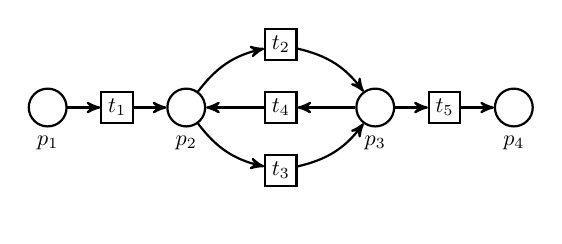
\begin{tikzpicture}[->,>=stealth',auto,x=10mm,y=1cm,node distance=11mm and 3mm,thick,  every node/.style={scale=0.8}]
		
		\node[pl,label = below:$p_1$]              (p1) {};
		\node[tr,right of = p1, label=center:$t_1$] (t1) {};
		\node[pl,right of = t1, label=below:$p_2$] (p2) {};
		
		\node[tr,right of = p2, label=center:$t_2$,yshift=1cm,xshift=4mm]  (t2) {};
		\node[tr,right of = p2, label=center:$t_3$,yshift=-1cm,xshift=4mm] (t3) {};
		\node[pl,right of = t2, label=below:$p_3$,yshift=-1cm,xshift=4mm] (p3) {};
		\node[tr,left  of = p3, label=center:$t_4$,xshift=-4mm] (t4) {};
		
		\node[tr,right of = p3, label=center:$t_5$] (t5) {};
		\node[pl,right of = t5, label=below:$p_4$] (p4) {};
		
		% Empty node to fix caption overlap
		% change yshift to LOWER value to make whitespace LESS
		\node[below of = t3,yshift=5mm] (a) {};
		
		\path[->]
		(p1) edge (t1)
		(t1) edge (p2)
		
		(p2) edge[bend left  = 20] (t2)
		(t2) edge[bend left = 20] (p3)
		
		(p2) edge[bend right = 20] (t3)
		(t3) edge[bend right = 20] (p3)
		
		(p3) edge (t4)
		(t4) edge (p2)

		(p3) edge (t5)
		(t5) edge (p4)
		;  
	\end{tikzpicture}
	\caption{%
		An example block-structured \wfnet. Each block corresponds to a node in the Jackson type
		$
		\jnsequence{
			p_1
		}{
			\jnsequence{
				t_1
			}{
				\jnsequence{
					\jnselfloop{
						\jnsequence{
							p_2
						}{
							\jnsequence{
								\jnchoice{t_2}{t_3}
							}{
								p_3
							}
						}
					}{
						t_4
					}
				}{
					\jnsequence{
						t_5
					}{
						p_4
					}
				}
			}
		}
		$. As example, the choice between transitions $t_2$ and $t_3$ corresponds to the node %
		$
		\jnsequence{p_2}{\jnsequence{\jnchoice{t_2}{t_3}}{p_3}}
		$
		.
	}
	\label{fig:example_wfnet}
\end{figure}

%\newcommand{\ptsequence}[1]{\ensuremath \rightarrow \left( #1 \right)}
%\newcommand{\ptselfloop}[2]{\ensuremath \circlearrowleft \left( #1 , #2 \right)}
%\newcommand{\ptparallel}[1]{\ensuremath \wedge \left( #1 \right)}
%\newcommand{\ptchoice}[1]{\ensuremath \times \left( \right)}


\subsection{Jackson Nets} \seclabel{jackson_nets}
% Hierarchical WFN
Whereas \wfnets do not put any restriction on the control flow of activities, block-structured \wfnets divide the control flow in logical blocks~\cite{KoppMWL15_DifferenceGraphBlockStructure}. Each ``block'' represents a single unit of work that can be performed, where this unit of work is either atomic (single transition), or one involving multiple steps (multiple transitions). 
An example block-structured \wfnet is shown in \figref{example_wfnet}.
The main advantage of block-structured \wfnets, is that the block-structure ensures that the \wfnet is sound by definition~\cite{KoppMWL15_DifferenceGraphBlockStructure,Leemans2013,vanHee2009}.
%An example block-structured \wfnet is shown in \figref{example_wfnet}. %
%Block-structured \wfnets can be represented by process trees~\cite{Leemans2013}. 
%A process tree is a rooted tree, where leaves represent activities and intermediate nodes represent operators. 
%Process trees describe a particular language, and its operators describe the semantics of how the languages of the subtrees (which are process trees) are to be combined.
%
%\begin{definition}[Process Tree~\cite{Leemans2013}] \deflabel{process_tree}
%	Let $\A$ be an alphabet of activities, and $\bigoplus = \set{\ptsequenceop, \ptparallelop,\ptchoiceop,\ptselfloopop}$ a set of operators, standing for sequences, parallelism, choices, and loops, respectively~\cite{Leemans2013}.
%	A \emph{process tree} is defined recursively: any $a \in \A$ is a process tree, and given  $M_1, \ldots, M_n$ for $n > 0$  process trees, and $\oplus \in \bigoplus$ an operator, then $\oplus\left(M_1, \ldots, M_n\right)$ is a process tree.
%\end{definition}
%
%\jmw{Add semantics of process trees}
%
%We consider the set of operators  This set of operators translates to well-structured, free-choice \pns~\cite{vanderAalst2000}.
%
%An example process tree, and its semantics as a Petri net is depicted in \figref{example_wfnet}. 
%The root of the process tree is the sequence operator ($\ptsequenceop$) on five sub trees, where $t_1$, $t_8$ and $t_{11}$ are leaves, and 
%$\ptselfloop{ 
%	\ptchoice{
%		\ptsequence{t_2, t_3 },
%		\ptsequence{t_4, t_5 }
%	}
%}{ t_6, t_7 }$
%and
%$\ptparallel{
%	t_9, t_{10}
%}$ 
%are two sub process trees inside the sequence operator.
%\db{Paragraph: explanation of example / Describe the example better; change figure to add something for the individual blocks}
%In the caption of \figreffull{example_wfnet}, we state directly its corresponding process tree. The construction of this process tree is relatively straightforward. When looking at the \wfnet, one can see that the first executed transition is $t_1$. Then, sequentially ($\rightarrow$), there is an entire block that is looped ($\circlearrowleft$); in the loop body a choice ($\times$) must be made between sequences $\rightarrow (t_2, t_3)$ or $\rightarrow (t_4, t_5)$, and looping itself can be achieved using either $t_6$ or $t_7$. After any number of loops (including 0), the process can (sequentially) continue with the execution of $t_8$, after which there is parallel ($\wedge$) execution of $t_9$ and $t_{10}$. The process ends with the final transition $t_{11}$. It is now easy to see that the process tree corresponding to the \wfnet from \figreffull{example_wfnet} is indeed $\rightarrow \left(t_1, \circlearrowleft \left(\times \left(\rightarrow \left(t_2, t_3\right), \rightarrow \left(t_4, t_5\right)\right), t_6, t_7\right), t_8, \wedge \left(t_9, t_{10}\right), t_{11}\right)$.
%As two process trees with different structures can express the same behavior, the following rewrite rules are used to define a normal forms, i.e., if two process trees have the same behavior, they have isomorphic normalized process tree.
%
%\begin{definition}[Normal Form for Process Trees~\cite{Leemans2013}] \proplabel{property_10_leemans}
%	Given a process tree, its normal form is derived by transforming it according to following identities:
%	\begin{eqnarray}
%		\oplus(M) & \equiv & M  \label{itm:pt1}\\
%		\times (\cdots_1, \times (\cdots_2), \cdots_3) & \equiv & \times(\cdots_1, \cdots_2, \cdots_3) \label{itm:pt2}\\
%		\rightarrow (\cdots_1, \rightarrow (\cdots_2), \cdots_3) & \equiv & \rightarrow(\cdots_1, \cdots_2, \cdots_3) \label{itm:pt3}\\
%		\wedge (\cdots_1, \wedge (\cdots_2), \cdots_3) & \equiv & \wedge(\cdots_1, \cdots_2, \cdots_3) \label{itm:pt4}\\
%		\circlearrowleft(\circlearrowleft(M, \cdots_1), \cdots_2) & \equiv & \circlearrowleft(M, \cdots_1, \cdots_2) \label{itm:pt5}\\
%		\circlearrowleft(M, \cdots_1, \times(\cdots_2), \cdots_3)  & \equiv & \circlearrowleft(M, \cdots_1,\cdots_2,\cdots_3)  \label{itm:pt6}
%	\end{eqnarray}
%%	Note that the underlying idea of these identities is to combine multiple nested subtrees with the same operator into a single node.
%\end{definition}
%
%\begin{example} \exlabel{example_wfnet_process_tree}
%	Process tree corresponding to the model shown in \figref{example_wfnet}.
%	$$
%	\rightarrow \left(t_1, \circlearrowleft \left(\times \left(\rightarrow \left(t_2, t_3\right), \rightarrow \left(t_4, t_5\right)\right), \times\left(t_6, t_7\right)\right), t_8, \wedge \left(t_9, t_{10}\right), t_{11}\right)
%	$$
%	Note that we have made explicit the choice in loopback paths by applying \propref{property_10_leemans}.
%\end{example}
%
%Different notations exist to represent block-structured \wfnets.
In this paper, we consider Jackson Types and Jackson Nets~\cite{vanHee2009}. 
A Jackson Type is a data structure used to capture all information involved in a single execution of a \wfnet. 

%\begin{definition}[Jackson Types~\cite{vanHee2009}] A \emph{Jackson type} \J is defined recursively by $\J ::= \mathscr A \mid (\J;\J) \mid {(\J||\J)} \mid (\J+\J) \mid (\J\#\J)$, where $\mathscr{A} = \mathscr{ A}^{p} \cup \mathscr{A}^{t} = \left\{a, b, c, \ldots \right\}$ denotes two disjoint sets of atomic types for places and transitions, resp., and symbols $;, ||, +, \#$ stand for types in sequence, parallelism, choices, and loops
%\end{definition}

\begin{definition}[Jackson Type~\cite{vanHee2009}]
	The set of \emph{Jackson Types} $\J$ is recursively defined by the following grammar: %recursively as:
	\begin{align*}
		\J & ::= \mathscr A ^p \mid 
		\jnsequence{\mathscr A^p}{\jnsequence{\J^t}{\mathscr A^p}}
		\\
		\J^t & ::= \mathscr A ^t \mid 
		\jnsequence{\J^t}{\jnsequence{\J^p}{\J^t}}
		\mid \jnchoice{\J^t}{\J^t} \\
		\J^p & ::= \mathscr A ^p \mid 
		\jnsequence{\J^p}{\jnsequence{\J^t}{\J^p}} \mid 
		\jnparallel{\J^p}{\J^p} \mid 
		\jnselfloop{\J^p}{\J^t}
	\end{align*}
where $\mathscr{A} = \mathscr{A}^{p} \cup \mathscr{A}^{t} = \left\{a, b, c, \ldots \right\}$ denotes two disjoint sets of atomic types for places and transitions, resp., and symbols $\jnsequenceop, \jnparallelop, \jnchoiceop, \jnselfloopop$ stand for sequence, parallelism, choices, and loops.
%Note how these correspond with the allowed graphical constructs of block-structured \wfnets.
\end{definition}

%As the operators in Jackson Types are all binary, an algebraic equivalence relation is defined to rewrite types into a normal form. \dbtodo{Some extra text explaining what this normal form is/does and why it's there? ; different types that represent the same model (also proved in paper Kees), but they have same behaviour. So: normal form to reason about a single thing.}
Multiple Jackson Types may exist for the same \wfnet.
For example, the Jackson Type
$
\jnsequence
{
	\jnsequence{p_1}{t_1}
}
{
	\jnsequence
	{
		\jnselfloop{
			\jnsequence{
				p_2
			}{
				\jnsequence{
					\jnchoice{t_2}{t_3}
				}{
					p_3
				}
			}
		}{
			t_4
		}
	}
	{
		\jnsequence{t_5}{p_4}
	}
}
$
describes the \wfnet of \figref{example_wfnet} as well.
%Since a \wfnet may have multiple Jackson types, we use a normal form.
Each net has a unique representation~\cite{vanHee2009}, called its normal form.
We define an algebraic equivalence between types to allow rewriting into the normal form.
%The normalized Jackson type essentially pushes all parentheses to the right by employing the identities from \defref{algebraic_equivalence}.
\begin{definition}[Algebraic equivalence, normal form~\cite{vanHee2009}] \deflabel{algebraic_equivalence}
The \emph{algebraic\\ equivalence} $\algequiv$ is the smallest equivalence relation on the set of Jackson Types that satisfies the following six rules:
\begin{equation*}\begin{array}{rclcrcl}                                                                                 %
	\jnsequence{\jnsequence{J_0}{J_1}}{J_2} & \algequiv & \jnsequence{J_0}{\jnsequence{J_1}{J_2}} &\  &  %
\jnchoice{\jnchoice{J_0}{J_1}}{J_2} & \algequiv & \jnchoice{J_0}{\jnchoice{J_1}{J_2}} \\                 %
\jnparallel{\jnparallel{J_0}{J_1}}{J_2} & \algequiv & \jnparallel{J_0}{\jnparallel{J_1}{J_2}} &\  &      %
\jnchoice{J_0}{J_1} & \algequiv & \jnchoice{J_1}{J_0} \\                                                 %
\jnparallel{J_0}{J_1} & \algequiv & \jnparallel{J_1}{J_0} & \  &                                          %
\jnselfloop{\jnselfloop{J_0}{J_1}}{J_2} & \algequiv & \jnselfloop{J_0}{\jnselfloop{J_1}{J_2}}            %
\end{array}
\end{equation*}
with $J_0, J_1, J_2 \in \J$ three Jackson Types.

A Jackson Type is in \emph{normal form} iff all brackets are moved to the right using the above rules.
\end{definition}
%
%%\subsection{Jackson nets} \seclabel{jackson_nets}
%%JACKSON NET
%While process trees show nicely the relation between different activities, they are unable to represent any information regarding the data flow corresponding to the process. Jackson nets (\jns) -- a specific type of colored {\pn} -- make data information explicit. They are based upon the set of Jackson types, which rest upon the concept of a (data) type. A \emph{type} \J is defined as $\J ::= \mathscr A \mid (\J;\J) \mid {(\J||\J)} \mid (\J+\J) \mid (\J\#\J)$, where $\mathscr{A} = \mathscr{ A}^{p} \cup \mathscr{A}^{t} = \left\{a, b, c, \ldots \right\}$ denotes a set of atomic types for places and transitions, respectively, and symbols $;, ||, +, \#$ stand for types in sequence, parallelism, choices, and loops~\cite{vanHee2009}. 

%\begin{property}[Algebraic Equivalence on Types~\cite{vanHee2009}] \proplabel{algebraic_equivalence_types}
%	Two types are algebraic equivalent if they abide by the identity rules:
%	\begin{eqnarray}
%		(J_0 ; J_1) ; J_2 & \equiv_{alg} & J_0 ; (J_1 ; J_2) \label{itm:jn_identity1} \\ 
%		(J_0 {||} J_1) {||} J_2 & \equiv_{alg} & J_0 {||} (J_1 {||} J_2) \label{itm:jn_identity2}\\ 
%		J_0 {||} J_1 & \equiv_{alg} & J_1 {||} J_0 \label{itm:jn_identity3} \\ 
%		(J_0 + J_1) + J_2 & \equiv_{alg} & J_0 + (J_1 + J_2) \label{itm:jn_identity4} \\ 
%		J_0 + J_1 & \equiv_{alg} & J_1 + J_0  \label{itm:jn_identity5} \\ 
%		(J_0 \# J_1) \# J_2 & \equiv_{alg} & J_0 \# (J_1 + J_2) \label{itm:jn_identity6}
%	\end{eqnarray}
%	with $J_0, J_1, J_2 \in \J$ three (potentially identical) types.
%\end{property}




%Notice how these four constructs seem to correspond with the four operators $\set{\rightarrow, \wedge,\times,\circlearrowleft}$ from \defref{process_tree}. 

%\db{Two types (not Jackson types) are algebraic equivalent if following holds ...}

%As to obtain a type that is valid for a block-structured \wfnet, we constrain the allowed operators between types such that, among others, a type for a place is always followed by a type of a transition, and vice versa. The set of constrained types are the \emph{Jackson Types}. Realize that since the algebraic equivalence rules in \propref{algebraic_equivalence_types} are defined for arbitrary types, they hold for Jackson types as well.

%\db{Different notation from original paper: they use $\tau$ for a single Jackson type, but we want to use that for a silent step (? Do we?). So, I've decided to simply make all normal J's calligraphic, and then write single type with capital J.}

The class of Jackson Nets is obtained by recursively applying \emph{generation rules}, starting from a singleton net with only one place. 
These generation rules are similar to those defined by Murata~\cite{Murata1989} and preserve soundness~\cite{vanHee2009}. 
%Indeed, it is shown that the generation rules for \jns too preserve soundness, and as such \jns are sound by construction~\cite{vanHee2009}.
Thus, any Jackson Net is sound by construction. 

\begin{definition}[Jackson Net~\cite{vanHee2009}] \deflabel{jackson_net}
	A \wfnet $N = (\places, \transitions, \flow, \inp, \outp)$ is called a \emph{Jackson Net} if it can be generated from a single place $p$ by applying the following five generation rules recursively:
%	\begin{enumerate}[label=J\arabic*]%, wide = 0pt, leftmargin=\parindent]
%		\item \label{itm:jn_R1} Sequential place split: %$\ell(p_1) = \left(\ell (p_2) ; \left(\ell (t_1) ; \ell (p_3)\right)\right)$
%		$p \leftrightarrow \jnsequence{p_1}{\jnsequence{t}{p_2}}$
%		\item \label{itm:jn_R2} Sequential transition split: 
%		%$\ell(t_1) = \left(\ell (t_2) ; \left(\ell (p_1) ; \ell (t_3)\right)\right)$
%		$ t \leftrightarrow \jnsequence{t_1}{\jnsequence{p_1}{t_2}}$
%		\item \label{itm:jn_R3} Loop Addition: 
%		%$\ell(p_1) = \left( \ell(p_2)\# \ell(t_1)\right)$
%		$p \leftrightarrow \jnselfloop{p}{t}$
%		\item \label{itm:jn_R4} AND split:  
%		%$\ell(p_1) = \left( \ell(p_2) ||  \ell(p_3)\right)$
%		$p \leftrightarrow \jnparallel{p_1}{p_2}$
%		\item \label{itm:jn_R5} OR split: 
%		%$\ell(t_1) = \left( \ell(t_2) +  \ell(t_3)\right)$
%		$ t \leftrightarrow \jnchoice{t_1}{t_2}$
%	\end{enumerate}
\begin{equation*}
	\begin{array}{llcll}
\mbox{J1:} & p \leftrightarrow \jnsequence{p_1}{\jnsequence{t}{p_2}} & \ \  &
\mbox{J4:} & p \leftrightarrow \jnparallel{p_1}{p_2}\\
\mbox{J2:} & t \leftrightarrow \jnsequence{t_1}{\jnsequence{p_1}{t_2}} & &
\mbox{J5:} & t \leftrightarrow \jnchoice{t_1}{t_2} \\
\mbox{J3:} & p \leftrightarrow \jnselfloop{p}{t} & & & \\
\end{array}
\end{equation*}
We say that $N$ is generated by $p$.
\end{definition}

As shown in~\cite{vanHee2009}, Jackson Nets are completely determined by Jackson Types, and vice versa. 

\begin{theorem}[Jackson Nets and Jackson Types are equivalent~\cite{vanHee2009}]
Let $N_1$ and $N_2$ be two Jackson Nets that are generated by the Jackson Types $J_1$ and $J_2$, resp. Then $N_1$ and $N_2$ are isomorphic iff $J_1 \algequiv J_2$.
\end{theorem}
%\db{Change below paragrah: don't use example but let text flow; refer to the main image top right for the model itself; then explain shortly where this sequence part comes from. }
%It should be noted that these generation rules for Jackson nets can also be used for reduction. For example, 
%In the Jackson net in the top right of \figref{process_tree_to_jackson_net_overview} we observe  the structure $(t_2;p_3;t_3)$ as the leftmost child node of the loop body. Using \ref{itm:jn_R1} we can reduce the sequence to a single (new) transition $t$, obtaining a new (sound) Jackson Net.

%\begin{example} \exlabel{example_wfnet_jackson_net}
%	Jackson type corresponding to the model shown in \figref{example_wfnet}.%
%	\vspace{0.2em}
%	\begin{dmath*}
%		\left(\ell\left(p_1\right);\left(\ell\left(t_1\right);\left(\ell\left(p_2\right)\#\left(\left(\ell\left(t_2\right);\left(\ell\left(p_3\right);\ell\left(t_3\right)\right)\right)+\left(\ell\left(t_4\right);\left(\ell\left(p_4\right);\ell\left(t_5\right)\right)\right)\right)\right); \\
%		\left(\left(\ell\left(t_6\right)+\ell\left(t_7\right)\right);\left(\ell\left(p_5\right);\left(\ell\left(t_8\right);\left(\ell\left(p_6\right);\left(\ell\left(t_9\right);\ell\left(p_7\right)\right)\right)||\left(\ell\left(p_8\right);\left(\ell\left(t_{10}\right);\ell\left(p_9\right)\right)\right)\right); \\
%		\left(\ell\left(t_{11}\right);\ell\left(p_{10}\right)\right)\right)\right)\right)\right)
%	\end{dmath*}%
%	\vspace{0.2em}
%	% Note that to obtain this \jn we have applied the algebraic equivalence from \propref{algebraic_equivalence_vanhee}, to make the choice in loopback paths explicit.
%\end{example}


%\begin{property}[Definition 6 from~\cite{vanHee2009}] \proplabel{algebraic_equivalence_vanhee}
%	Let $a, b, c \in \mathscr{A}$ three atomic types. Then the following holds, where $\equiv_{alg}$ denotes algebraic equivalence.
%	$$
%	\left(a \# \left(b \# c \right) \right) \equiv_{alg} a \# \left(b + c\right)
%	$$
%\end{property}


%\subsection{Jackson Nets are Process Trees} \seclabel{jns_are_pts}

%.{\seqarr}  $t_1$ {\looparr} $t_8$ $\wedge$ $t_0$ $t_{10}$ $t_{11}$]
%\begin{figure}[t]
%	\centering
%	\begin{tikzpicture}[sibling distance=-2pt, level distance = 18pt,scale=0.7]
%		\begin{scope}
%			\node[yshift=4mm](N1){\textsf{\textbf{Process tree}}};
%			\Tree [.{\seqarr}  [.\node(T1a1){$t_1$}; ] [.{\looparr} [.$\times$ [.{\seqarr} $t_2$ $t_3$ ] [.{\seqarr}  $t_4$ $t_5$ ] ] $t_6$ $t_7$ ] [.$t_8$ ]  [.$\wedge$ $t_9$ $t_{10}$ ] [.\node(T1a2){$t_{11}$}; ]  ]
%			\node[above of = T1a1,yshift=-2mm](a1t1){};
%			\node[right of = T1a2,yshift=-18mm,xshift=.6cm](a2t1){};
%			\node[below of = N1,yshift=-13mm] (e1){};
%		\end{scope}
%		
%		
%		\begin{scope}[yshift=-6.2cm]
%			\node[yshift=4mm](N2){\textsf{\textbf{Explicit loopback paths}}};
%			\Tree [.{\seqarr}  [.\node(T2a1){$t_1$}; ] [.{\looparr} [.$\times$ [.{\seqarr} $t_2$ $t_3$ ] [.{\seqarr}  $t_4$ $t_5$ ] ] [.$\times$ $t_6$ $t_7$ ] ] [.$t_8$ ]  [.$\wedge$ $t_9$ $t_{10}$ ] [.\node(T2a2){$t_{11}$}; ]  ]
%			\node[above of = T2a1,yshift=-1mm,xshift=-1mm](a1t2){};
%			\node[right of = T2a2,yshift=24mm,xshift=8mm](a2t2){};
%			\node[above of = N2,yshift=-6mm] (e2){};
%			\node[below of = N2,xshift=19mm] (ee2){};
%		\end{scope}
%		
%		
%		\draw [Triangle-Triangle,thick,green1] (e1) --node[right]{(a)}++ (e2);
%		
%		\begin{scope}[xshift=10cm, level 1/.style={level distance=35pt}]
%			\node[yshift=4mm](N3){\textbf{\textsf{Jackson Type}}};
%			\Tree [.{;}  \node(T3a1){$p_1$};   $\hspace{3em}t_1\hspace{3em}$ [.$\hspace{-3em}\#\hspace{-3em}$ $\hspace{-6em}p_2\hspace{-6em}$ [.; [.$+$ [.; $t_2$ $p_3$ $t_3$ ] [.; $t_4$ $p_4$ $t_5$ ] ] [.$\hspace{-2em}+\hspace{-2em}$ $t_6$ $t_7$ ] $p_5$  ] ] $\hspace{-1em}t_8\hspace{-1em}$ [.||  [.; $p_6$ $t_9$ $p_7$ ] [.; $p_8$ $t_{10}$ $p_9$ ] ]   $\hspace{3em}t_{11}\hspace{3em}$ \node(T3a2){$p_{10}$}; ]
%			\node[above of = T3a1,yshift=3mm](a1t3){};
%			\node[right of = T3a2,yshift=-23mm,xshift=-37mm](a2t3){};
%			\node[below of = N3,yshift=-22mm] (e3){};
%		\end{scope}
%		
%		\begin{scope}[yshift=-6.2cm,xshift=10cm]
%			\node[yshift=4mm](N4){\textsf{\textbf{Reduced Normal Form}}};
%			\Tree [.{;}  \node(T4a1){$t_1$};  [.$\#$  [.$+$ [.; $t_2$ $t_3$ ] [.; $t_4$ $t_5$ ]  ]    [.$+$ $t_6$ $t_7$  ]  ] $t_8$ [.||   $t_9$  $t_{10}$  ]   \node(T4a2){$t_{11}$}; ]
%			\node[above of = T4a1,yshift=-1mm](a1t4){};
%			\node[right of = T4a2,yshift=24mm,xshift=-6.3cm](a2t4){};
%			\node[above of = N4,yshift=-6mm] (e4){};
%			\node[below of = N4,xshift=-18mm] (ee4){};
%		\end{scope}
%		
%		\draw [Triangle-Triangle,thick,byzantium] (e3) --node[right]{(b)}++ (e4);
%		\draw [Triangle-Triangle,thick,cadmiumorange] (ee2) --node[above]{(c)}++ (ee4);
%		
%		\begin{pgfonlayer}{background}
%			\filldraw [line width=4mm,join=round,cadmiumorange!20]
%			(a1t1.north west) rectangle ++(a2t1.south east)
%			(a1t2.north west) rectangle ++(a2t2.south east);
%			\filldraw [line width=4mm,join=round,blue-violet!20]
%			(a1t3.north west) rectangle ++(a2t3.south east)
%			(a1t4.north west) rectangle ++(a2t4.south east);
%		\end{pgfonlayer}
%		
%	\end{tikzpicture}
%	\caption{Visual illustration of the proof for \thmref{process_tree_is_jackson_net}: arrow \textcolor{green1}{\textbf{(a)}} normalizes the process tree, and makes loopback paths explicit. Arrow \textcolor{byzantium}{\textbf{(b)}} reduces and normalizes the Jackson type to its reduced normal form. Arrow \textcolor{cadmiumorange}{\textbf{(c)}} denotes the isomorphism.}
%	\label{fig:process_tree_to_jackson_net_overview}
%\end{figure}

%Process trees, Jackson Types and Jackson Nets are three representations for block-structured \wfnets. 
%In the remainder of this subsection, we prove that these representations are algebraic equivalent.
%The idea of the proof is visualised in \figref{process_tree_to_jackson_net_overview}.



%Here, the process tree (top left) has implicit loopback paths. In step \textcolor{BurntOrange}{\textbf{(a)}} these are made explicit by applying \propref{property_10_leemans}. The Jackson type (top right) has been constructed to also show the explicit choice in loopback paths by application of \propref{algebraic_equivalence_vanhee}. Step \textcolor{OliveGreen}{\textbf{(b)}} is a reduction operation defined on Jackson types, and \textcolor{Fuchsia}{\textbf{(c)}} denotes the relation between symbols. In other words, these are (in practice) the three required steps necessary to show that a process tree is equivalent to the Jackson type of a \jn.

%\begin{enumerate}[label=(\alph*)]
%	\item Make choices of loopback paths explicit for the loop operator.
%	\item Reduce the Jackson type (ensure that loopback paths are explicit) to its reduced form, while keeping control flow actions.
%	\item Map operators from process trees to those used by Jackson types and vice versa.
%\end{enumerate}

%\begin{figure}
%	\centering
%	\includegraphics[width=0.9\linewidth]{figs/process_tree_to_jackson_net_overview}
%	\caption{Illustration of steps taken to show that process trees are equivalent to Jackson nets.}
%	\label{fig:process_tree_to_jackson_net_overview}
%\end{figure}

%\dbtodo{Fix "equivalent" here; what do we consider to be equivalent? -> The underlying workflow nets are isomorphic}
%We argue that process trees are equivalent to the Jackson type of a \jn. The equivalence relation we consider is isomorphism between the underlying \wfnets of the process tree and the Jackson type. This is best demonstrated by the running example in \figreffull{process_tree_to_jackson_net_overview}. The process tree in the top left shows \textit{implicit loopback paths} in the loop block $\circlearrowleft(\cdots, t_6, t_7)$: either path $t_6$ or path $t_7$ is chosen. Clearly, there is a choice ($\times$) between these two loopback paths. By applying identity \ref{itm:pt6} from \propref{property_10_leemans} one can rewrite such that this choice is made explicit: $\circlearrowleft(\cdots, t_6, t_7)$ becomes $\circlearrowleft(\cdots, \times (t_6, t_7))$. We make the loopback paths explicit after transforming the process tree to the normal form, indicated by the arrow annotated with \textcolor{green1}{\textbf{(a)}}. As such, the resulting process tree in the bottom left is thus the normal form with explicit loopback paths.
%We also normalize the Jackson type in the top right. The Jackson type is first normalized, and then reduced to its reduced normal form. This normalization and reduction is denoted by the arrow annotated with \textcolor{byzantium}{\textbf{(b)}}.
%After transorming the top models into the bottom ones, it becomes clear that, for this example, the process tree and Jackson type on the bottom of the figure are indeed equivalent; the only difference is the symbols used for the (same) operations. The equivalence relation is denoted by \textcolor{cadmiumorange}{\textbf{(c)}}. We formalize this idea into \thmreffull{process_tree_is_jackson_net}, where we proof that, indeed, after transformations process trees and Jackson types are equivalent.




%REDUCED TYPE FROM VANHEE
%Jackson types are used to derive case trees fully describing the data attributes at each atomic action taken in a workflow. To derive a case tree, the original Jackson type is modified -- reduced -- to remove nodes that refer to places. After places are removed, the reduced Jackson type is simplified by removing superfluous sequence operator nodes. Note that control flow steps are usually also removed when creating a reduced Jackson type, as these do not have corresponding steps in the data flow. For our purpose, we keep actions that are solely describing control flow. The reduction of the Jackson type corresponds to the \textcolor{OliveGreen}{\textbf{green}} arrow labeled \textcolor{OliveGreen}{\textbf{(b)}} in \figreffull{process_tree_to_jackson_net_overview}.

%CREATE FUNCTION THAT MAPS OPERATORS
%\begin{definition} \deflabel{process_tree_to_jackson_net_relation}
%	Let $G$ be a relation such that $\set{(\rightarrow, ;), (\times, +), (\circlearrowleft, \#), (\wedge, ||)} \subseteq G$.
%\end{definition}

%When comparing the reduced Jackson type (with kept control flow actions) to the process tree showing the explicit choice between loopback paths, it becomes clear that these models are identical. As such, we propose \thmref{process_tree_is_jackson_net}.
%This is formalized by means of relation $F$ from \defreffull{process_tree_to_jackson_net_relation}: each operator used in process trees maps one-to-one with an operator used in the Jackson type. By exchanging the operators from one model to another, again a valid model is obtained, either as reduced Jackson type or as process tree with explicit loopback paths. The application of $G$ from either side corresponds to the \textcolor{Fuchsia}{\textbf{purple}} arrow labeled  \textcolor{Fuchsia}{\textbf{(c)}} in \figreffull{process_tree_to_jackson_net_overview}.

%\db{How to formalize this as a proof?}

%\begin{theorem}
%Process trees are a subclass of Jackson nets.
%\end{theorem}
%\andy{\textbf{we need to rewrite the theorem}\\ 
%the main idea: given a process tree, we can construct a jackson net that is equivalent to it\\
%translate process trees to jackson types}

%\db{Some connecting text here?}

%We formalize the above example into \thmreffull{process_tree_is_jackson_net}. Essentially, we take identical steps to those from \figreffull{process_tree_to_jackson_net_overview}, and show that the arrow denoted by \textcolor{cadmiumorange}{\textbf{(c)}} is an isomorphic equivalence (on the underlying \wfnets of the respective models).

%\begin{theorem} \thmlabel{process_tree_is_jackson_net}
%	Two process trees 
%	Given a process tree $\mathcal T$, we can construct a Jackson Net $N$ such that the underlying \wfnets of $\mathcal T$ and $N$ are isomorphic.
%	Process trees and Jackson nets are algebraic equivalent: let $\T$ a process tree, then we can construct a Jackson Net $N$ such that $\T \equiv_{alg} N$.
%\end{theorem}

%Algebraic equivalence means that the normal forms of process trees and Jackson types are isomorphic. You can rewrite A into B according to some rules, and the rules necessary here is just the mapping of operators.

%\db{Connecting paragraph sketching the proof?}
%\begin{proof}
%%	\dbtodo{TODO: Proof; see commented latex for previous attempt.}
%	Let $\T$ be a process tree. We define a \emph{place-fusing operator} as follows. Let $N = (\places_N, \transitions_N, \flow_N)$ and $M = (\places_M, \transitions_M, \flow_M)$ be two \emph{disjoint} \pns, and let $r: \places_N \to \places_M$ an injective function. Then $N \bowtie_{r} = (\places, \transitions, \flow)$ is their \emph{place-fused} \pn with $\places = \left(\places_N \union \places_M \right) \setminus \dom{r}$, $\transitions = \transitions_N \union \transitions_M$, and $\flow = \left(\flow_N\union \flow_M\right) \setminus \Union_{q \in \dom{r}} \left( \left( \set{q} \times \post{q} \right) \union \left( \pre {q}\times \set{q} \right) \right) \union \Union_{(p, q) \in r} \left( \left( \set{p} \times \post{q} \right) \union \left( \pre {p}\times \set{q} \right) \right) $.
%	We now show that, given $\T$,  we can construct an algebraic equivalent Jackson type, where algebraic equivalence means that we can ``rewrite'' the process tree to the Jackson type using the identities from \propref{property_10_leemans} (process trees) and \propref{algebraic_equivalence_types} (Jackson types). In fact, we only have to show equivalence between the process tree and the \emph{reduced} Jackson type, as the we can always invert the reduction back to its original Jackson type.
%	We consider following five cases:
%	\begin{case} \textbf{Single activity}.\\
%		In this case, $\T = t$, with $t$ some activity. Then trivially a reduced Jackson type exists that is algebraic equivalent: $t$.
%	\end{case}
%	\begin{case} \textbf{Sequence}. \\
%		In this case, $\T = {\rightarrow \left(\T_1, \T_2\right)}$ a sequence of sub-blocks \dbtodo{subtrees?} $\T_1$ and $\T_2$. By induction, there exist \jns $N$ and $M$ for $\T_1$ and $\T_2$ respectively. Then, place-fused $N \bowtie_{\{(out_N, in_M)\}\}} M$ has as corresponding reduced Jackson type $\J = (\T_1 ; \T_2)$. Clearly $\T$ and $\J$ are algebraically equivalent, their only differences laying in infix/prefix notation, and the symbol used for denoting sequences.
%	\end{case}
%	\begin{case} \textbf{Choice}. \\
%		\dbtodo{should come before loops since we use choices in the loops}
%	\end{case}
%	\begin{case} \textbf{Loop}. \\
%		In this case, $\T = {\circlearrowleft \left(\T_1, \T_2\right)}$, that is, the structured loop of the sub-block $\T_1$ with (potentially multiple) loopback path(s) $\T_2$. By induction, there exist \jns $N$ and $M$ for $\T_1$ and $\T_2$ respectively. Then, place-fused $N \bowtie_{\{(in_N, out_M), (out_N, in_M)\}\}} M$ has as corresponding Jackson type $\J = (\T_1\#\T_2)$. If $\T_2$ consists of a single activity, then clearly $\J$ and $\T$ are algebraically equivalent. Otherwise, when $\T_2$ consists of more than one activity, one must make loopback paths explicit by introducing the choice. However, since we have already shown algebraic equivalence for the choice operator in previous case, there again must exist an algebraic equivalent reduced Jackson type.
%	\end{case}
%\end{proof}

%To prove \thmreffull{process_tree_is_jackson_net}, we define a \textit{place-fusing operation} that takes two PNs, and returns a new PN with places fused according to an injective function $r$. 
 
%\begin{definition} \deflabel{merge_operator}
%	Let $N = (\places_N, \transitions_N, \flow_N)$ and $M = (\places_M, \transitions_M, \flow_M)$ be two \emph{disjoint} \pns,
%	and let $r: \places_N \to \places_M$ an injective function. Then $N \bowtie_{r} = (\places, \transitions, \flow)$
%	is their \emph{place-fused} \pn with $\places = \left(\places_N \union \places_M \right) \setminus \dom{r}$, $\transitions = \transitions_N \union \transitions_M$, and $\flow = \left(\flow_N\union \flow_M\right) \setminus \Union_{q \in \dom{r}} \left( \left( \set{q} \times \post{q} \right) \union \left( \pre {q}\times \set{q} \right) \right) \union \Union_{(p, q) \in r} \left( \left( \set{p} \times \post{q} \right) \union \left( \pre {p}\times \set{q} \right) \right) $.
%\end{definition}

%\db{Proof sketch of inductive proof:
%- briefly discuss single activity for PT and JN
%- are they the same: yes
%- repeat for sequence, choice, loop, parallel}
%\db{Is the proof just the same as the above paragraph, but then "in general"? So, first make loopback paths explicit, if they are present, by applying the property. Then, define function that maps symbols from process trees to jackson nets. How do we then get to "this is a reduced Jackson type"?}
%\dbtodo{Rewrite of proof still required}
%\begin{proof}
%	Let \T be a process tree corresponding to \wfnet $M_\T = (\places, \transitions, \flow, in, out)$. We can construct Jackson Net $N$ such that its underlying \wfnet $M_N$ is isomorphic to $M_\T$. 
%	% Single activity
%	\begin{case} \textbf{Single activity}. \\
%		In this case, $\T = a$, that is, a single activity $a$. Then $(\set{i, o}, \set{a}, \set{(i, a), (a, o)}, i, o, \ell)$ is the corresponding \jn, with $\ell(in);\ell(a);\ell(out)$ its Jackson type.
%	\end{case}
%	\begin{case} \textbf{Sequence}. \\
%		In this case, $\T = {\rightarrow \left(\T_1, \T_2\right)}$, that is, a sequence of process trees $\T_1$ and $\T_2$. By induction, there exist \jns $N$ and $M$ for $\T_1$ and $\T_2$ respectively. Then, place-fused $N \bowtie_{\{(out_N, in_M)\}\}} M$ is the Jackson type of its corresponding \jn. Bisimilarity follows directly from \defref{merge_operator}.
%	\end{case}
%	\begin{case} \textbf{Choice}. \\
%		In this case, $\T = {\times \left(\T_1, \T_2\right)}$, that is, the choice of process trees $\T_1$ and $\T_2$. By induction, there exist \jns $N$ and $M$ for $\T_1$ and $\T_2$ respectively. Then, place-fused $N \bowtie_{\{(in_N, in_M), (out_N, out_M)\}\}} M$ is the Jackson type of its corresponding \jn. Bisimilarity follows directly from \defref{merge_operator}.
%	\end{case}
%	\begin{case} \textbf{Loop}. \\
%		In this case, $\T = {\circlearrowleft \left(\T_1, \T_2\right)}$, that is, the structured loop of process tree $\T_1$ with (potentially multiple) loopback path(s) $\T_2$. By induction, there exist \jns $N$ and $M$ for $\T_1$ and $\T_2$ respectively. Then, place-fused $N \bowtie_{\{(in_N, out_M), (out_N, in_M)\}\}} M$ is the Jackson type of its corresponding \jn. Bisimilarity follows directly from \defref{merge_operator}.
%	\end{case}
%	\begin{case} \textbf{Parallel}. \\
%		In this case, $\T = {\wedge \left(\T_1, \T_2\right)}$, that is, the interleaved execution of process trees $\T_1$ and $\T_2$. By induction, there exist \jns $M$ and $O$ for $\T_1$ and $\T_2$ respectively. \dbtodo{This needs to be written properly.}
%		% Construct new Nackson net; this is a workflow net.
%		We construct Jackson net $N = (\places_N, \transitions_N, \flow_N, in_N, out_N)$ from $N_1$ and $N_2$ such that $\places_N = \places_M \union \places_O \union \set{in_N, out_N}$, $\transitions_N = \transitions_M \union \transitions_O \union \set{\tau_1, \tau_2}$ where $\tau_1$ and $\tau_2$ are silent steps, and $\flow_N = \flow_M \union \flow_O \union \set{(in_N, \tau_1), (\tau_1, in_M), (\tau_1, in_O), (out_M, \tau_2), (out_O, \tau_2), (\tau_2, out_N)}$. \dbtodo{We need to define what a marking is, what the firing rule is, and what enabledness is, for \jns; for now I'm just assuming I can use these.}
%		% Define relation for bisimulation
%		We define $Q \subseteq \markings{\T} \times \markings{N}$ such that $(m_\T, m_N) \in Q \implies \forall p \in P: m_\T(p) = m_N(p)$ \dbtodo{perhaps we need a slightly different notion here due to types of places; depends on what a marking is for jackson nets}.
%		% State what we want to show
%		Let $(m_\T, m_N) \in Q$, and $\fire{(\T, m_\T)}{t}{(\T, m_\T')}$ for some arbitrary $t \in \transitions$.
%		We need to show that there exists some $m_N'$ such that $\fire{(N, m_N)}{t}{(N, m_N')}$, and that $(m_\T', m_N') \in Q$.
%		% Actual proof
%		Since $(m_\T, m_N) \in Q$, and $\fire{(\T, m_\T)}{t}{(\T, m_\T')}$, by definition of $Q$ there must exist some $m_N'$ obtained after firing $t$ from $m_N$ \dbtodo{Is this true?}. As such, $\fire{(N, m_N)}{t}{(N, m_N')}$.
%		That $(m_\T', m_N') \in Q$ follows directly from the firing rules and the definition of $Q$ \dbtodo{probably need some more argumentation here}.
%		\dbtodo{This proves one direction; still need to do the other one where there is no longer strong bisim due to $\tau$.}
%	\end{case}
%\end{proof}

\subsection{Petri Nets with Identifiers} \seclabel{petrinets_identifiers}
% Systems as petri nets with identifiers
Whereas \wfnets describe all possible executions for a single case, 
systems typically consist of many interacting processes.
The latter can be modeled using typed Petri nets with identifiers (\tpnids for short)~\cite{vanderWerf2022}.
In this formalism, each object is typed and has a unique identifier to be able to refer to it.
Tokens carry vectors of identifiers, which are used to relate objects.
Variables on the arcs are used to manipulate the identifiers.
% Sentence below is already too verbose?
%\dbtodo{We define sets of identifiers, type labels, and variables in \defref{identifier_types}.}

\begin{definition}[Identifiers, Types and Variables] \deflabel{identifier_types}
	Let \idset, \labelset, and \varset denote countably infinite sets of identifiers, type labels, and variables, respectively. We define:
	\begin{compactitem}
			\item the \emph{domain assignment} function $I : \labelset \rightarrow \powerset{\idset}$, such that $I(\lambda_1)$ is an infinite set, and $I(\lambda_1) \cap I(\lambda_2) \neq \emptyset$ implies $\lambda_1 = \lambda_2$ for all $\lambda_1, \lambda_2 \in \labelset$;
			\item the \emph{id typing} function $\type_{\idset}:\idset\to\labelset$ s.t.\ if $\type_{\idset}(\cname{id})=\lambda$, then $\cname{id}\in I(\lambda)$;
			\item a \emph{variable typing} function $\type_{\varset}:\varset\to\labelset$, prescribing that $x\in\varset$ can be substituted only by values from $I(\type_{\varset}(x))$.
		\end{compactitem}
	When clear from the context, we omit the subscripts of $\type$.
	We lift the $\type$ functions to sets, vectors, and sequences by applying the function on each of its constituents.
\end{definition}

In a \tpnid, each place is annotated with a label, called the \emph{place type}.
A place type is a vector of types, indicating types of identifier tokens the place can carry. Similar to Jackson Types, we use $\jnplace{p}{\lambda}$ to denote that place $p$ has type $\alpha(p) = \lambda$.
%\dbtodo{We use $[p, \lambda]$ to denote a place $p$ with $\alpha(p) = \lambda$.}
%Using $\alpha$, places are annotated with its place type.
%We write $\jnplace{p}{\lambda}$ for place $p$ with place type $\lambda$.
%A place with an empty place type, represented by the empty vector, is a classical Petri net place carrying indistinguishable (black) tokens.
Each arc is inscribed with a multiset of vectors of identifiers, such that the type of each variable coincides with the place types.
%This allows to model situations in which a transition may require multiple tokens with different identifiers from the same place.
%Using $\beta$, arcs are annotated with vectors of variables called \emph{inscriptions}. 
If the inscription is empty or contains a single element, we omit the brackets. 

\begin{definition}[Typed Petri net with identifiers] \deflabel{tpnids}
	A \emph{typed Petri net with identifiers} (\tpnid) $N$ is a tuple $(\places,\transitions,\flow,\alpha,\beta)$, where:
	\begin{compactitem}
			\item $(\places,\transitions,\flow)$ is a classical Petri net;
			\item $\alpha: \places \to \labelset^*$ is the \emph{place typing function};%, if $\alpha(p) = \emptysequence$, place $p$ can only carry black, i.e., uncolored, tokens;
			\item $\beta : \flow \to \setmult{(\varset^*)}$ defines for each arc a multiset of \emph{variable vectors} s.t.\ $\alpha(p) = \type(x)$ for any $x \in \setsupp{\beta((p,t))}$ and $\type(y)=\alpha(p')$ for any $y \in \setsupp{\beta((t,p'))}$ where $t\in\transitions$, $p\in\pre{t}$, $p'\in\post{t}$.
		\end{compactitem}
\end{definition}

%In the remainder of the paper we assume there exists a bijection on variables ($\varset$) and types ($\labelset$), and that there are no `classical' places: $\size{\alpha(p)} > 0$ for all $p \in P$.
%If an event log does not specify a type corresponding to a variable, then we say that these are equal.
%Since an event log is a sequence of events for a certain object type, we need to make the above assumptions to avoid undefined sequences without object type.
%We assign a Gödel-like number $\godelsymb$ to each type to impose an ordering on arc inscriptions: if $\lambda = \sequence{x, y, z}$, then $\godel{x} < \godel{y} < \godel{z}$. 
%The induced total order is required to extend the notion of a normal form for Jackson nets to typed Jackson nets.
%Since the order of a type can be deduced by $\godelsymb$, we can use sequence and set notation interchangeably for arc inscriptions.

% TPNID semantics
A marking of a \tpnid is the configuration of tokens over the set of places.
Each token in a place should be of the correct type, i.e., the vector of identifiers carried by a token in a place should match the corresponding place type.
The set $\colset(\place)$ defines all possible vectors of identifiers a place $p$ may carry.

\begin{definition}[Marking] \deflabel{marking}
	Given a \tpnid $N = (\places, \transitions, \flow, \alpha, \beta)$, and place $\place \in \places$, its \emph{id set} is $\colset(\place) = \prod_{1 \leq i \leq |\alpha(\place)|} I(\alpha(\place)(i))$.
	A \emph{marking} is a function $\marking \in \markings{N}$, with $\markings{N} = \places \to \setmult{(\seq{\labelset})}$, such that $\marking(\place) \in \setmult{\colset(p)}$, for each place $\place \in \places$. The set of identifiers used in $\marking$ is denoted by $\Id(\marking) = \Union_{\place \in \places} \rng{\setsupp{\marking(\place)}}$
	The pair \markednet{N}{\marking} is called a \emph{marked \tpnid}.
\end{definition}

To define the semantics of a \tpnid, the variables need to be valuated with identifiers.

\begin{definition}[Variable sets~\cite{vanderWerf2022}] \deflabel{variable_sets}
	Given a \tpnid $N=(\places,\transitions,\flow,\alpha,\beta)$, $t\in \transitions$ and $\lambda \in \Lambda$, we define the following sets of variables:
	\begin{compactitem}
		\item \emph{input variables} as $\smash{\invar{t} = \bigcup_{x \in \beta((p,t)), p\in\pre{t}} \rng{\setsupp{x}}}$;
		\item \emph{output variables} as $\smash{\outvar{t} = \bigcup_{x \in \beta((t,p)),p \in\post{t}} \rng{\setsupp{x}}}$;
		\item \emph{variables} as $\var{t} = \invar{t} \cup \outvar{t}$;
		\item \emph{emitting variables} as $\newvar{t} = \outvar{t}\setminus\invar{t}$;
		\item \emph{collecting variables} as $\delvar{t} = \invar{t} \setminus \outvar{t}$;
		\item \emph{emitting transitions} as $E_N(\lambda) = \{ t \mid \exists x \in \newvar{t} \wedge \type(x) = \lambda \}$;
		\item \emph{collecting transitions} as $C_N(\lambda) = \{ t \mid \exists x \in \delvar{t} \wedge \type(x) = \lambda \}$;
		\item \emph{types in $N$} as \smash{$\type(N) = \{ \vec\lambda \mid \exists p \in P : \vec\lambda\in\alpha(p)\}$}.
	\end{compactitem}
\end{definition}

%As customary in colored Petri nets, the firing of a transition requires a \emph{binding} that valuates variables to identifiers.
A valuation of variables to identifiers is called a \emph{binding}.
Bindings are used to inject new fresh data into the net via variables that emit identifiers, i.e., via variables that appear only on the output arcs of that transition.
%We require bindings to be an injection, i.e., no two variables within a binding may refer to the same identifier.
Note that in this definition, freshness of identifiers is local to the marking, i.e., disappeared identifiers (those fully removed from the net through collecting transitions) may be reused, as it does not hamper the semantics of the \tpnid.
%Our semantics allow the use of well-ordered sets of identifiers, such as the natural numbers, as used in~\cite{Polyvyanyy2019,RosaVelardo2006} to ensure that identifiers are globally new.
%Here we assume local freshness over global freshness.

\begin{definition}[Firing rule for \tpnids]
 	Given a marked \tpnid $(N,m)$ with $N=(\places,\transitions,\flow,\alpha,\beta)$, a \emph{binding} for  transition $t\in T$ is an injective function  $\psi:\V\rightarrow \I$ such that
 	$\type(v) = \type(\psi(v))$
 	and
 	$\psi(v)\not\in \Id(m)$ iff $v\in\newvar{t}$.
 	Transition $t$ is \emph{enabled} in $(N,m)$ under binding $\psi$, denoted by $\pnenabled{(N,m)}{t,\psi}$ iff $\rho_\psi(\beta(p,t)) \leq m(p)$ for all $p\in\pre{t}$.
 	Its firing results in marking $m'$, denoted by $\fire{(N,m)}{t,\psi}{(N, m')}$, such that $m'(p) + \rho_\psi(\beta(p,t)) = m(p) + \rho_\psi(\beta(t,p))$. %for %$p \in \places$.%, for every $p\in\pre{t}\cup\post{t}$.
% 	The set of all finite firing sequences 
\end{definition}
The firing rule is inductively extended to sequences.
A marking $m'$ is \emph{reachable} from $m$ if there exists $\eta\in (\transitions\times(\V\rightarrow \I))^*$ such that $\fire{(N,m)}{\eta}{(N,m')}$.
 %For a marked \tpnid $(N,M)$, we denote with $\reachable{N}{M}$  the set of all markings reachable from $M$.
We denote with $\pnreachable{N}{m}$ the set of all markings reachable from $m$ for $\markednet{N}{m}$.
%\db{New text from here to def 10.}
We use $\L\markednet{N}{m}$ to denote all possible firing sequences of \markednet{N}{m}, i.e., $\L\markednet{N}{m} = \{\eta \mid \pnenabled{(N,m)}{\eta}{}\}$ and $\Id(\eta) = \bigcup_{(t,\psi) \in \eta} \rng{\psi}$ for the set of identifiers used in $\eta$.
The execution semantics of a \tpnid is defined as an LTS that accounts for all possible executions starting from a given initial marking.
We say two \tpnids are bisimilar if their induced transition systems are.

 \begin{definition}
	     Given a marked \tpnid $(N,m_0 )$ with $N=(P,T,F,\alpha,\beta)$, its induced transition system  is $\transitionsystem{N,m_0} = (\mathbb{M}(N),(T\times(\V\to\I)),m_0 , \to)$ with $m\xrightarrow{(t,\psi)} m'$ iff  $\fire{\markednet{N}{m}}{t,\psi}{\markednet{N}{m'}}$.
%	     \begin{compactitem}
%	     	 \item $S=\pnreachable{N}{m_0 }$ and $s_0=m_0 $,
%	     	 \item for $M,M^\prime\in S$ it holds that: 
%	     	 	$M\xrightarrow{(t,\psi)} M^\prime$ iff  $\fire{\marking}{t,\psi}{\marking^\prime}$. %for $t\in\transitions$ and binding $\sigma$. 
%	     \end{compactitem}
\end{definition}


%\dbtodo{Paragraph on indentifier soundness and why we care; make link with Jackson Nets as final note.}
Soundness properties for \wfnets typically consist of proper completion, weak termination, and quasi-liveness~\cite{AalstHHS11_soundness}. 
Extending soundness to \tpnids gives \emph{identifier soundness}~\cite{vanderWerf2022}.
%By extending to \tpnids, proper completion becomes proper type completion, and weak termination becomes weak type termination.
%The first intuitively means that objects of type $\lambda$ are created by emitters, and once consumed by a collector all objects with the same type should be consumed.
%Proper type completion intuitively means that the life-cycle of each type is proper completing: an object of a given type ``enters'' the system through an emitting transition, binding it to a unique identifier.
%Once a collecting transition fires, there should be no remaining tokens referring to the removed object.
%Weak type termination intuitively means that it should always be possible to eventually remove a type by firing a collecting transition.
In \tpnids, each object of a given type ``enters'' the system through an emitting transition, binding it to a unique identifier.
Identifier soundness intuitively states that it should always be possible to remove objects (weak type termination), and that once a collecting transition fires for an object, there should be no remaining tokens referring to the removed object (proper type completion). 

%\begin{definition}[Identifier Soundness~\cite{vanderWerf2022}]
%	Let $\markednet{N}{m_0}$ a marked \tpnid and $\lambda \in \Lambda$ some type.
%	$\markednet{N}{m_0}$ is \emph{$\lambda$-sound} iff it is
%	\begin{inparaenum}[\it (i)]
%		\item proper $\lambda$-completing, i.e., for all $t \in C_N(\lambda)$, bindings $\psi : \V\to\I$ and markings $m, m'\in\pnreachable{N}{m_0}$, if $\fire{m}{t,\psi}{m'}$, then for all identifiers $\cname{id} \in \rng{\restr{\psi}{\delvar{t}}} \cap \Id(m)$ and $\type(\cname{id})=\lambda$, it holds that $\cname{id}\not\in\Id(m')$\footnote{Here, we constrain $\psi$ only to objects of type $\lambda$ that are only consumed.};
%		\item weakly $\lambda$-terminating, i.e.,  for every $m \in \pnreachable{N}{m_0}$ and identifier $\cname{id} \in I(\lambda)$ such that $\cname{id} \in \Id(m)$, there exists a marking $m' \in \pnreachable{N}{m}$ with $\cname{id} \not\in \Id(m')$.
%	\end{inparaenum}
%	If it is $\lambda$-sound for all $\lambda\in \type(N)$, then it is \emph{identifier sound}.
%\end{definition}

\begin{definition}[Identifier Soundness~\cite{vanderWerf2022}]
	Let $\markednet{N}{m_0}$ a marked \tpnid and $\lambda \in \Lambda$ some type.
	$\markednet{N}{m_0}$ is \emph{$\lambda$-sound} iff it is
	\begin{compactitem}
		\item Proper $\lambda$-completing, i.e., for all $t \in C_N(\lambda)$, bindings $\psi : \V\to\I$ and markings $m, m'\in\pnreachable{N}{m_0}$, if $\fire{m}{t,\psi}{m'}$, then for all identifiers $\cname{id} \in \rng{\restr{\psi}{\delvar{t}}} \cap \Id(m)$ and $\type(\cname{id})=\lambda$, it holds that $\cname{id}\not\in\Id(m')$ \footnote{Here, we constrain $\psi$ only to objects of type $\lambda$ that are only consumed.};
		\item Weakly $\lambda$-terminating, i.e.,  for every $m \in \pnreachable{N}{m_0}$ and identifier $\cname{id} \in I(\lambda)$ such that $\cname{id} \in \Id(m)$, there exists a marking $m' \in \pnreachable{N}{m}$ with $\cname{id} \not\in \Id(m')$.
	\end{compactitem}
	If it is $\lambda$-sound for all $\lambda\in \type(N)$, then it is \emph{identifier sound}.
\end{definition}

	% \begin{definition}[Weak type termination]
		%     \label{def:termination}
		%     Given type $\lambda\in\Lambda$, a marked \tpnid $(N, M_0)$ is called \emph{weakly $\lambda$-terminating} iff
		%     for every $M \in \reachable{N}{M_0}$ and identifier $\cname{id} \in I(\lambda)$ such that $\cname{id} \in \id{M}$, there exists a marking $M' \in \reachable{N}{M}$ with $\cname{id} \not\in \id{M'}$.
		% \end{definition}
	
%	Given type $\lambda\in\Lambda$, a marked \tpnid $(N, M_0)$ is called \emph{proper $\lambda$-completing} iff for all $t \in C_N(\lambda)$, bindings $\psi : \V\to\I$ and markings $M, M'\in\reachable{N}{M_0}$, if $\fire{M}{t,\psi}{M'}$, then for all identifiers $\cname{id} \in \rng{\restr{\psi}{\delvar{t}}} \cap \id{M}$ and $\type(\cname{id})=\lambda$, it holds that $\cname{id}\not\in\id{M'}$.\footnote{Here, we constrain $\psi$ only to objects of type $\lambda$ that are only consumed.}
	
%	A marked \tpnid $(N,M_0)$ is \emph{$\lambda$-sound} iff it properly $\lambda$-completes and weakly $\lambda$-terminates.
%	It is \emph{identifier sound} iff it is $\lambda$-sound for every $\lambda\in \type(N)$.
	


% Each type has a life-cycle.
% Intuitively, an object of a given type ``enters'' the system via an emitter that creates a unique identifier that refers to the object.
% The identifier remains in the system, until the object ``leaves'' the system by firing a collecting transition (that binds to the identifier and consumes it).
% Hence, once that transition fires, there should be no remaining tokens referring to the removed object.
% The process of a type is a model that describes all possible paths allowed for a type.
% It can be represented as a transition-bordered WF-net~\cite{HeeSW13}.
% Instead of a sink and source place, a transition-bordered WF-net has transitions that represent the start and finish of a process.
% A transition-bordered WF-net is sound, if its closure is sound.
% As shown in Fig.~\ref{fig:tBorderedNet}, its closure is constructed by creating a new source place $i$ s.t. each emitting transition consumes from $i$, and a new sink place $f$ s.t. each collecting transition produces in $f$.
% Consider in \tpnid $N_{\mathit{rs}}$ of Fig~\ref{fig:overallModel}, identifier type $\mathit{order}$. Its life cycle starts with transition $G$. Transitions $K$ and~$V$ are two transitions that may remove the last reference to an $\mathit{order}$. Soundness of a transition-bordered WF-net would require that firing transition $K$ or transition $V$ would result in the final marking.
% In the remainder of this section, we develop this intuition into the concept of identifier soundness.


% Soundness constitutes three properties: proper completion, weak termination and quasi-liveness.
% Similarly to~\cite{HeeSV03}, we focus on the first two properties.
% \emph{Proper completion} states that if a marking covers the final marking, it is the final marking. In other words, as soon as a token is produced in the final place, all other places are empty.
% Following the idea of transition-bordered WF-nets, identifiers should have a similar behavioral property: once an identifier is consumed by a collector, the identifier should be removed from the marking.

% \begin{definition}[Proper type completion]
	%     Given type $\lambda\in\Lambda$, a marked \tpnid $(N, M_0)$ is called \emph{proper $\lambda$-completing} iff for all $t \in C_N(\lambda)$, bindings $\psi : \V\to\I$ and markings $M, M'\in\reachable{N}{M_0}$, if $\fire{M}{t,\psi}{M'}$, then for all identifiers $\cname{id} \in \rng{\restr{\psi}{\delvar{t}}} \cap \id{M}$ and $\type(\cname{id})=\lambda$, it holds that $\cname{id}\not\in\id{M'}$.\footnote{Here, we constrain $\psi$ only to objects of type $\lambda$ that are only consumed.}
	% \end{definition}
% %we restrict identifiers to Collect(t) so as to admit situations with subnets where a transition has two input places p1 and p2, both of the same type, F={(p1,t),(p2,t),(t,p2)} and beta(p1,t)=x and beta(p2,t)=y (obviously, y shouldn't be touched in that case)

% As an example, consider \tpnid $N_{\mathit{rs}}$ in Fig.~\ref{fig:overallModel}.
% For type $\mathit{customer}$, %the set of collecting transitions is 
% we have $C_{N_{\mathit{rs}}}(\mathit{customer}) = \{K, V\}$.
% In the current -- empty -- marking, transition $T$ is enabled with binding  $\psi = \{y\mapsto \cname{o}, z\mapsto \cname{c}\}$, which results in marking $M$ with $M(\textit{customer}) = [\cname{c}]$.
% Next, transitions $G$, $H$, $J$, $L$ and $N$ can fire, all using the same binding,
% producing marking $M'$ with $M'(p) = [\cname{o},\cname{c}]$, $M'(\mathit{customer}) =[\cname{c}]$ and $M'(q) = M'(r) = [\cname{c}]$.
% Hence, transition $K$ is enabled with binding $\psi$.
% %As $K \in \C_{N_{rs}}(\mathit{customer})$, it is a collector for type $\mathit{customer}$. 
% However, firing $K$ with $\psi$ results in marking $M''$ with $M''(\mathit{customer}) = [\cname{c}]$, while $\psi(z) = \cname{c}$.
% Hence, $N_{\mathit{rs}}$ is not properly $\mathit{customer}$-completing.

% %\medskip
% \emph{Weak termination} for a WF-net signifies that from any reachable marking, the final marking can be reached.
% Translated to identifiers, it should always eventually be possible to remove an identifier from a marking.

% \begin{definition}[Weak type termination]
	%     \label{def:termination}
	%     Given type $\lambda\in\Lambda$, a marked \tpnid $(N, M_0)$ is called \emph{weakly $\lambda$-terminating} iff
	%     for every $M \in \reachable{N}{M_0}$ and identifier $\cname{id} \in I(\lambda)$ such that $\cname{id} \in \id{M}$, there exists a marking $M' \in \reachable{N}{M}$ with $\cname{id} \not\in \id{M'}$.
	% \end{definition}

% %\medskip
% \emph{Identifier soundness} combines the two properties of proper type completion and weak type termination: the former ensures that as soon a collector fires for an identifier, the identifier is removed, whereas the latter ensures that it is always eventually possible to remove that identifier.

% %By joining together the previous definitions we obtain the one of identifier soundness.
% \begin{definition}
	%     \label{def:soundness}
	%     A marked \tpnid $(N,M_0)$ is \emph{$\lambda$-sound} iff it properly $\lambda$-completes and weakly $\lambda$-terminates. It is \emph{identifier sound} iff it is $\lambda$-sound for every $\lambda\in \type(N)$.
	% \end{definition}

% There are two interesting observations that one can make about the identifier soundness property. First, identifier soundness does not imply soundness in the classical sense: any classical net $N$ without types, i.e., $\type(N) = \emptyset$, is identifier sound, independently of the properties of $N$.

%As we use \tpnids to model interacting processes, we assume in the remainder of this paper that each place corresponds to at least one process, i.e., $\alpha(p) \neq \emptyset$ for any place $p \in P$, 

\subsection{Typed Jackson Nets} \seclabel{typed_jackson_nets}
%\dbtodo{Needs different text! We don't look at process trees anymore.}
%Now that we have established that \jns are equivalent to process trees, we argue that \emph{typed} Jackson nets (\tjns) are a natural extension to \jns by adding identifiers $\cname{id} \in \I$, and thus are a natural extension to process trees. We show the extension of \jns explicitly in \defref{typed_jackson_net} by relating the generation rules for \jns to the generation rules for \tjns. 
In general, identifier soundness is undecidable for \tpnids~\cite{vanderWerf2022}.
Similar as Jackson Nets restrict \wfnets to blocks, \emph{typed Jackson Nets} (\tjns) restrict \tpnids to blocks, while guaranteeing identifier soundness and liveness. 
%A \emph{typed} Jackson net (\tjn) is a \tpnid that is sound and live by construction~\cite{vanderWerf2022}.
For \tjns, we disallow multiplicity on arcs and variables, i.e., $\beta(f)(v) \le 1$ for all $f \in F$ and $v \in \V$, and imply a bijection on variables and identifier types.
This prevents place types like $\lambda = \sequence{x, x}$.
Assuming a G\"odel-like number on types (cf.~\cite{vanHee2009}), place types and arc inscriptions can be represented as sets.
Similar as Jackson Types describe Jackson Nets, we apply a notation based on Jackson Types to denote typed Jackson Nets.

%We argue that \tjns are a natural extension to \jns by adding identifiers $\cname{id} \in \I$.
%We show the extension of \jns explicitly in \defref{typed_jackson_net} by relating the generation rules for \jns to the generation rules for \tjns.

%\andy{we need to be specific on how arc inscriptions relate to each other (no need in elaborating on types due to the bijection assumption)}
\begin{definition}[Typed Jackson Net] \deflabel{typed_jackson_net}
	A \tpnid $N$ is a \emph{typed Jackson Net} if it can be generated from a set of transitions $T'$ by applying any of the following six generation rules recursively. If $N$ is generated from a singleton set of transitions (i.e., $\length{T'} = 1$), $N$ is called \emph{atomic}. 
	
	\begin{enumerate}[label=R\arabic*, wide = 0pt, leftmargin=\parindent]
		\item \label{itm:tjn_R1} Place Expansion:
		$
		\jnplace{p}{\lambda} \leftrightarrow
		\jnsequence{
			\jnplace{p_1}{\lambda}
		}{
			\jnsequence{
				t_1
			}{
				\jnplace{p_2}{\lambda}
			}
		}$
		\begin{center}
			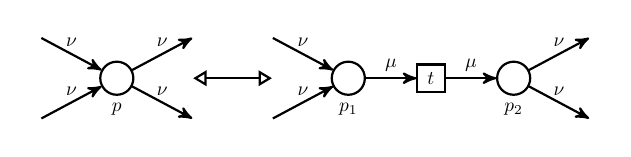
\begin{tikzpicture}[->,>=stealth',auto,x=17mm,y=1.3cm,node distance=15mm and 15mm,thick,  every node/.style={scale=0.7}]
				
				\node[pl,label = below:$p$] (p){};
				\node[left of = p,yshift=8mm](in1){};
				\node[left of = p,yshift=-8mm](in2){};
				\node[right of = p,yshift=8mm](out1){};
				\node[right of = p,yshift=-8mm](out2){};
				
				\path[->] 
				(in1) edge node[above]{$\nu$} (p)
				(in2) edge node[above]{$\nu$} (p)
				(p) edge node[above]{$\nu$} (out1)
				(p) edge node[above]{$\nu$} (out2)
				;  
				
				\node[pl,right of = p, xshift=2.7cm, label = below:$p_1$] (p1){};
				\node[tr,right of = p1, label = center:$t$] (t){};
				\node[pl,right of = t, label = below:$p_2$] (p2){};
				\node[left of = p1,yshift=8mm](in1){};
				\node[left of = p1,yshift=-8mm](in2){};
				\node[right of = p2,yshift=8mm](out1){};
				\node[right of = p2,yshift=-8mm](out2){};
				\path[->] 
				(in1) edge node[above]{$\nu$} (p1)
				(in2) edge node[above]{$\nu$} (p1)
				(p1) edge node[above]{$\mu$} (t)
				(t) edge node[above]{$\mu$} (p2)
				(p2) edge node[above]{$\nu$} (out1)
				(p2) edge node[above]{$\nu$} (out2)
				;  
				
				\draw[{Triangle[open]}-{Triangle[open]}] ([xshift=7.5mm]p.east) -- ([xshift=-7.5mm]p1.west) ;
				
			\end{tikzpicture}
		\end{center}
	
		\item \label{itm:tjn_R2} Transition Expansion:
		$
		t \leftrightarrow
		\jnsequence{
			t_1
		}{
			\jnsequence{
				\jnplace{p}{\lambda}
			}{
				t_2
			}
		}
		$%
		, with $\var{t} \subseteq \lambda$
		\begin{center}
			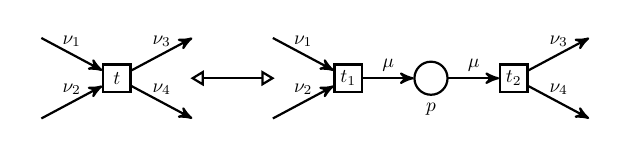
\begin{tikzpicture}[->,>=stealth',auto,x=17mm,y=1.3cm,node distance=15mm and 15mm, thick,  every node/.style={scale=0.7}]
				\node[tr,label = center:$t$] (t){};
				\node[left of = t,yshift=8mm](in1){};
				\node[left of = t,yshift=-8mm](in2){};
				\node[right of = t,yshift=8mm](out1){};
				\node[right of = t,yshift=-8mm](out2){};
				
				\path[->] 
				(in1) edge node[above]{$\nu_1$} (t)
				(in2) edge node[above]{$\nu_2$} (t)
				(t) edge node[above]{$\nu_3$} (out1)
				(t) edge node[above]{$\nu_4$} (out2)
				;  
				
				\node[tr,right of = t, xshift=2.7cm, label = center:$t_1$] (t1){};
				\node[pl,right of = t1, label = below:$p$] (p){};
				\node[tr,right of = p, label = center:$t_2$] (t2){};
				\node[left of = t1,yshift=8mm](in1){};
				\node[left of = t1,yshift=-8mm](in2){};
				\node[right of = t2,yshift=8mm](out1){};
				\node[right of = t2,yshift=-8mm](out2){};
				\path[->] 
				(in1) edge node[above]{$\nu_1$} (t1)
				(in2) edge node[above]{$\nu_2$} (t1)
				(t1) edge node[above]{$\mu$} (p)
				(p) edge node[above]{$\mu$} (t2)
				(t2) edge node[above]{$\nu_3$} (out1)
				(t2) edge node[above]{$\nu_4$} (out2)
				;  
				
				\draw[{Triangle[open]}-{Triangle[open]}] ([xshift=7.5mm]t.east) -- ([xshift=-7.5mm]t1.west) ;		
			\end{tikzpicture}
		\end{center}
	
		\item \label{itm:tjn_R3} Place Duplication:
		$
		\jnsequence{t_1}{\jnsequence{\jnplace{p}{\lambda}}{t_2}} \leftrightarrow
		\jnsequence{t_1}{\jnsequence{\jnparallel{\jnplace{p}{\lambda}}{\jnplace{p'}{\lambda'}}}{t_2}}
		$%
		, \\with $\lambda' \cap \newvar{\post{p}} = \emptyset$\\ 
		\begin{center}
			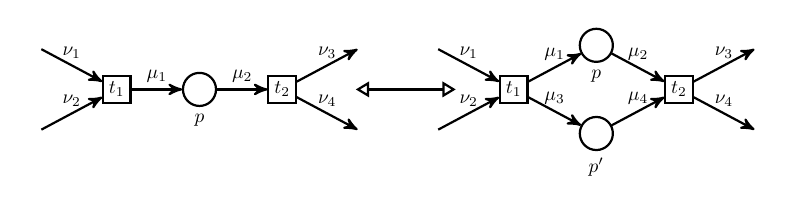
\begin{tikzpicture}[->,>=stealth',auto,x=17mm,y=1.3cm,node distance=15mm and 15mm, thick,  every node/.style={scale=0.7}]
				\node[tr, label = center:$t_1$] (t1){};
				\node[pl,right of = t1, label = below:$p$] (p){};
				\node[tr,right of = p, label = center:$t_2$] (t2){};
				\node[left of = t1,yshift=8mm](in1){};
				\node[left of = t1,yshift=-8mm](in2){};
				\node[right of = t2,yshift=8mm](out1){};
				\node[right of = t2,yshift=-8mm](out2){};
				\path[->] 
				(in1) edge node[above]{$\nu_1$} (t1)
				(in2) edge node[above]{$\nu_2$} (t1)
				(t1) edge node[above]{$\mu_1$} (p)
				(p) edge node[above]{$\mu_2$} (t2)
				(t2) edge node[above]{$\nu_3$} (out1)
				(t2) edge node[above]{$\nu_4$} (out2)
				;  
				
				
				
				\node[tr,right of = t2, xshift=2.7cm, label = center:$t_1$] (tt1){};
				\node[pl,right of = tt1, label = below:$p$,yshift=8mm] (p1){};
				\node[pl,right of = tt1, label = below:$p'$,yshift=-8mm] (p2){};
				\node[tr,right of = p1, label = center:$t_2$,yshift=-8mm] (tt2){};
				\node[left of = tt1,yshift=8mm](in1){};
				\node[left of = tt1,yshift=-8mm](in2){};
				\node[right of = tt2,yshift=8mm](out1){};
				\node[right of = tt2,yshift=-8mm](out2){};
				\path[->] 
				(in1) edge node[above]{$\nu_1$} (tt1)
				(in2) edge node[above]{$\nu_2$} (tt1)
				(tt1) edge node[above]{$\mu_1$} (p1)
				(p1) edge node[above]{$\mu_2$} (tt2)
				(tt1) edge node[above]{$\mu_3$} (p2)
				(p2) edge node[above]{$\mu_4$} (tt2)
				(tt2) edge node[above]{$\nu_3$} (out1)
				(tt2) edge node[above]{$\nu_4$} (out2)
				;  
				
				\draw[{Triangle[open]}-{Triangle[open]}] ([xshift=7.5mm]t2.east) -- ([xshift=-5.5mm]tt1.west) ;		
			\end{tikzpicture}
		\end{center}
	
		\item \label{itm:tjn_R4} Transition Duplication:
		$
		t \leftrightarrow 
		\jnchoice{t}{t'}
		$
		\begin{center}
			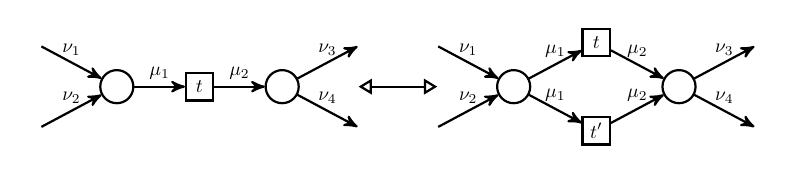
\begin{tikzpicture}[->,>=stealth',auto,x=17mm,y=1.3cm,node distance=15mm and 15mm, thick,  every node/.style={scale=0.7}]
				\node[pl] (p1){};
				\node[tr,right of = p1, label = center:$t$] (t){};
				\node[pl,right of = t, ] (p2){};
				\node[left of = p1,yshift=8mm](in1){};
				\node[left of = p1,yshift=-8mm](in2){};
				\node[right of = p2,yshift=8mm](out1){};
				\node[right of = p2,yshift=-8mm](out2){};
				\path[->] 
				(in1) edge node[above]{$\nu_1$} (p1)
				(in2) edge node[above]{$\nu_2$} (p1)
				(p1) edge node[above]{$\mu_1$} (t)
				(t) edge node[above]{$\mu_2$} (p2)
				(p2) edge node[above]{$\nu_3$} (out1)
				(p2) edge node[above]{$\nu_4$} (out2)
				;  
				
				\node[pl,right of = p2, xshift=2.7cm,] (pp1){};
				\node[tr,right of = pp1, label = center:$t$,yshift=8mm] (t1){};
				\node[tr,right of = pp1, label = center:$t'$,yshift=-8mm] (t2){};
				\node[pl,right of = t1,yshift=-8mm ] (pp2){};
				\node[left of = pp1,yshift=8mm](in1){};
				\node[left of = pp1,yshift=-8mm](in2){};
				\node[right of = pp2,yshift=8mm](out1){};
				\node[right of = pp2,yshift=-8mm](out2){};
				\path[->] 
				(in1) edge node[above]{$\nu_1$} (pp1)
				(in2) edge node[above]{$\nu_2$} (pp1)
				(pp1) edge node[above]{$\mu_1$} (t1)
				(t1) edge node[above]{$\mu_2$} (pp2)
				(pp1) edge node[above]{$\mu_1$} (t2)
				(t2) edge node[above]{$\mu_2$} (pp2)
				(pp2) edge node[above]{$\nu_3$} (out1)
				(pp2) edge node[above]{$\nu_4$} (out2)
				;  
				\draw[{Triangle[open]}-{Triangle[open]}] ([xshift=7.5mm]p2.east) -- ([xshift=-7.5mm]pp1.west) ;
			\end{tikzpicture}
		\end{center}
	
		\item \label{itm:tjn_R5} Self Loop Addition:
		$
		\jnplace{p}{\lambda} \leftrightarrow
		\jnselfloop{
			\jnplace{p}{\lambda}
		}{
			t
		}
		$
		\begin{center}
			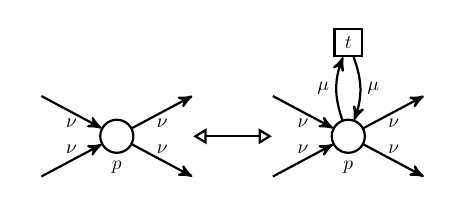
\begin{tikzpicture}[->,>=stealth',auto,x=17mm,y=1.3cm,node distance=15mm and 15mm,thick,  every node/.style={scale=0.7}]
				
				\node[pl,label = below:$p$] (p){};
				\node[left of = p,yshift=8mm](in1){};
				\node[left of = p,yshift=-8mm](in2){};
				\node[right of = p,yshift=8mm](out1){};
				\node[right of = p,yshift=-8mm](out2){};
				
				\path[->] 
				(in1) edge node[below]{$\nu$} (p)
				(in2) edge node[above]{$\nu$} (p)
				(p) edge node[below]{$\nu$} (out1)
				(p) edge node[above]{$\nu$} (out2)
				;  
				
				\node[pl,right of = p, xshift=2.7cm, label = below:$p$] (p1){};
				\node[tr,above of = p1, label = center:$t$,yshift=2mm] (t){};
				\node[left of = p1,yshift=8mm](in1){};
				\node[left of = p1,yshift=-8mm](in2){};
				\node[right of = p1,yshift=8mm](out1){};
				\node[right of = p1,yshift=-8mm](out2){};
				\path[->] 
				(in1) edge node[below]{$\nu$} (p1)
				(in2) edge node[above]{$\nu$} (p1)
				(p1) edge[bend left=20] node[left]{$\mu$} (t)
				(t) edge[bend left=20] node[right]{$\mu$} (p1)
				(p1) edge node[below]{$\nu$} (out1)
				(p1) edge node[above]{$\nu$} (out2)
				;  
				
				\draw[{Triangle[open]}-{Triangle[open]}] ([xshift=7.5mm]p.east) -- ([xshift=-7.5mm]p1.west) ;
				
			\end{tikzpicture}
		\end{center}
	
		\item \label{itm:tjn_R6} Identifier Introduction:
		$t \leftrightarrow
		\jnnewidentifier{t}{N_1}{\jnplace{p}{\lambda}}{N_2}
		$%
		, with
		$
		\jnsequence{N_1}{\jnsequence{\jnplace{p}{\lambda}}{N_2}}
		$ a \tjn and $\lambda \cap \var{t} = \emptyset$
		\begin{center}
			\begin{tikzpicture}[->,>=stealth',auto,x=17mm,y=1.3cm,node distance=15mm and 15mm,thick,  every node/.style={scale=0.7}]
				\node[tr,label = center:$t$] (t){};
				\node[left of = t,yshift=8mm](in1){};
				\node[left of = t,yshift=-8mm](in2){};
				\node[right of = t,yshift=8mm](out1){};
				\node[right of = t,yshift=-8mm](out2){};
				
				\path[->] 
				(in1) edge node[below]{$\nu_1$} (t)
				(in2) edge node[above]{$\nu_2$} (t)
				(t) edge node[below]{$\nu_3$} (out1)
				(t) edge node[above]{$\nu_4$} (out2)
				;  
				
				\node[tr,right of = p, xshift=2.7cm, label = center:$t$] (t1){};
				\node[pl,above of = t1, label = above:$p$,yshift=2mm] (p1){};
				\node[tr,left of = p1,label = center:$t_1$] (t2){};
				\node[tr,right of = p1,label = center:$t_2$] (t3){};
				\node[left of = t1,yshift=8mm](in1){};
				\node[left of = t1,yshift=-8mm](in2){};
				\node[right of = t1,yshift=8mm](out1){};
				\node[right of = t1,yshift=-8mm](out2){};
				\path[->] 
				(in1) edge node[below]{$\nu_1$} (t1)
				(in2) edge node[above]{$\nu_2$} (t1)
				(t1) edge[bend left=20] node[left]{$\mu$} (p1)
				(p1) edge[bend left=20] node[right]{$\mu$} (t1)
				(t2) edge node[above]{$\mu$} (p1)
				(p1) edge node[above]{$\mu$} (t3)
				(t1) edge node[below]{$\nu_3$} (out1)
				(t1) edge node[above]{$\nu_4$} (out2)
				;  
				
				\draw[{Triangle[open]}-{Triangle[open]}] ([xshift=7.5mm]t.east) -- ([xshift=-7.5mm]t1.west) ;
			\end{tikzpicture}
		\end{center}
	\end{enumerate}
\end{definition}

An example t-JN is given in \figref{runningexample}. 
Starting with the product process, transitions $C$ and $D$ can be reduced using rule $R2$. 
The resulting transition is a self-loop transition, and can be reduced using $R5$, resulting in the block $\jnnewidentifier{E}{A}{\mathit{product}}{B}$.
This block can be reduced using $R6$, leaving transition $E$.
Transition $E$ is again a self-loop, and can be reduced using $R5$.
The block containing transitions $H$, $J$, $L$ $O$, $N$ and $K$ can be reduced to a single place by applying rules $R1$, $R2$ and $R5$ repeatedly. 
The remaining place is a duplicate place with respect to place $p$, and can be reduced using $R3$.
Applying $R2$ on $G$ and $Z$ results in the block $\jnnewidentifier{G}{T}{\mathit{customer}}{V}$, 
which can be reduced to the transition $G$. 
Hence, the net in \figref{runningexample} is an atomic \tjn.
%\db{Paragraph on that rules R1-R5 are trivially the same as J1-J5 for jackson nets; then explain why we need to use the triple for R6 (example in PDF by JM)}

\begin{theorem}[Identifier Soundness of typed Jackson Nets \cite{vanderWerf2022}] \thmlabel{tjn-is-identifier-sound}
	Given a \tjn $N$, then $N$ is \emph{identifier sound} and \emph{live}.
\end{theorem}

%\db{Give example of reduction, based on the running example Jackson net}
%It should be noted that these generation rules for \tjns can also be used for reduction, as is the case with \jns.

%The generation rules for \tjns can also be used for reduction, as is the case with \jns.
%For instance, in the \tjn depicted in \figref{tjn_example}, we observe the structure
%$\jnsequence{t_1}{\jnsequence{\jnplace{p_3}{\lambda}}{t_4}}$.
%By applying \ref{itm:tjn_R2} we can reduce this sequence to a single (new) transition obtaining a new \tjn, hence it is atomic.
%
%\begin{figure}[H]
%	\centering
%	\begin{tikzpicture}[->,>=stealth',auto,x=10mm,y=1cm,node distance=11mm and 3mm,thick,  every node/.style={scale=0.8}]
%		\node[tr,label = center:$t_1$]               (t1) {};
%		\node[pl,right of = t1, label=below:$p_3$]  (p3) {};
%		\node[tr,right of = p3, label=center:$t_4$] (t4) {};
%		\node[pl,right of = t4, label=below:$p_1$]  (p1) {};
%		\node[tr,right of = p1, label=center:$t_3$,yshift=1cm, xshift=0.2cm] (t3) {};
%		\node[tr,below of = t3, label=center:$t$,yshift=-1cm]   (t)  {};
%		\node[pl,right of = t3, label=below:$p_1$,yshift=-1cm, xshift=0.2cm]  (p2) {};
%		\node[tr,right of = p2, label=center:$t_2$] (t2) {};
%		
%		% Empty node to fix caption overlap
%		% change yshift to LOWER value to make whitespace LESS
%		\node[below of = t,yshift=5mm] (a) {};
%		
%		\path[->]
%		(t1) edge node[above]{$x$} (p3)
%		(p3) edge node[above]{$x$} (t4)
%		(t4) edge node[above]{$x$} (p1)	
%		
%		(p1) edge[bend left = 20] node[below]{$x$} (t3)
%		(t3) edge[bend left = 20] node[below]{$x$} (p2)
%		(p2) edge[bend left = 20] node[above]{$x$} (t)
%		(t)  edge[bend left = 20] node[above]{$x$} (p1)
%		(p2) edge node[above]{$x$} (t2)
%		;
%	\end{tikzpicture}
%	\caption{An example \tjn, notated as
%		$
%		\jnnewidentifier{
%			t
%		}{
%			\jnsequence{
%				t_1
%			}{
%				\jnsequence{
%					\jnplace{p_3}{\lambda}
%				}{
%					t_4
%				}
%			}
%		}{
%			\jnplace{p_1}{\lambda}
%		}{
%			\jnsequence{
%				t_3
%			}{
%				\jnsequence{
%					\jnplace{p_2}{\lambda}
%				}{
%					t_2
%				}
%			}
%		}
%	$.}
%	\figlabel{tjn_example}
%\end{figure}

%TODO:
%\jmw{Add the text in comments below in the journal extension}
%It is trivial to see that rules \ref{itm:tjn_R1} to \ref{itm:tjn_R5} correspond directly with rules \textit{J1} to \textit{J5} from \defref{jackson_net}. 
%Hence, we state that \tjns are a natural extension to the \jns due to the addition of \ref{itm:tjn_R6}. 
%%By adding \ref{itm:tjn_R6}, we have transformed Murata rules~\cite{Murata1989} to object-centric process mining.
%This new rule, however, cannot use ``simple notation'' $t \leftrightarrow \left(t \triangleleft \left( t_1; [p, \lambda]; t_2\right)\right)$, since it then becomes unclear to which place transition $t$ is connected. 
%We demonstrate this issue by using (wrong) ``simple notation'' in following example.
%Consider the \tjn $\left(t \triangleleft \left( t_1; [p, \lambda]; t_2\right)\right)$, where we have just applied \ref{itm:tjn_R6} on transition $t$.
%Applying \ref{itm:tjn_R1} on $p$, followed by \ref{itm:tjn_R2} on $t_1$ we obtain $\left(t \triangleleft \left(t_1 ; \left( \left[p_3, \lambda\right] ; t_2 \right) ; \left( \left[p_1, \lambda\right] ; \left( t_3; \left[p_2, \lambda\right]\right);t_2\right)\right)\right)$ as shown in \figreffull{tjn_example}.
%When rewriting to its normal form $\left(t \triangleleft \left(t_1 ; \left( \left[ p_3, \lambda \right] ; \left( t_4 ; \left( \left[p_1, \lambda\right] ; \left( t_3 ; \left( \left[p_2, \lambda\right] ; t_2 \right)\right)\right)\right)\right)\right)\right)$ it is no longer clear to which place transition $t$ is connected to.
%As such, the notation is defined with a triple as shown in \ref{itm:tjn_R6}, which avoids this ambiguity.

% it is trivial to see that any JN can be transformed to a tJN by simply not using R6 and a mapping of lambdas}

%\db{Final paragraph; nice link with Murata (also has 6 rules), easy (trivial) to make sound models, good mathematical foundation.}

%\dbtodo{Maybe a corollary stating that tJN are a natural extension to JN?}


%\begin{figure}[H]
%	\centering
%	\includegraphics[width=0.99\textwidth]{figs/new_notation_for_typed_jackson_nets.png}
%	\caption{Extending Jackson net notation to typed Jackson Nets}
%	\label{fig:tjn_extends_jn_notation}
%\end{figure}
%




%
%\db{Anything below here is old}
%
%
%\db{To introduce t-JNs we have to talk about t-PNIDs; TYPED PNIDs; Note: lots of copy paste happens here; this should be rewritten to avoid plagiarism}
%
%\db{FLOW: Jackson nets -> typed JN}
%The class of typed Jackson nets (\tjns) are a subset of all typed \pns with identifiers (\tpnids), constructed in such a way that they are identifier sound~\cite{Werf2022}. A typed \pn with identifers itself extends the $\nu$-PNs~\cite{RVFE11} by allowing tokens to carry vectors of identifiers. Identifiers are typed: the countable, infinite set of identifiers is partitioned into a set of types, such that each type contains a countable, infinite set of identifiers. Variables are typed as well and can only refer to identifiers of the associated type.
%

%
%TYPED-JACKSON Nets
%
%PROOF: TYPED JACKSON NETS ARE A NATURAL EXTENSION OF PROCESS TREES:
%EVERY PROCESS TREE IS A TYPED JACKSON NET
%\db{Proof: process tree -> Jackson net -> typed Jackson net}
%



% %%%%%%%%%%% EVERYTHING BELOW THIS LINE IS COPY PASTED
% As customary in colored Petri nets, the firing of a transition requires a \emph{binding} that valuates variables to identifiers.
% The binding is used to inject new fresh data into the net via variables that emit identifiers, i.e., via variables that appear only on the output arcs of that transition.
% We require bindings to be an injection, i.e., no two variables within a binding may refer to the same identifier.
% Note that in this definition, freshness of identifiers is local to the marking, i.e., disappeared identifiers may be reused, as it does not hamper the semantics of the \tpnid.
% Our semantics allow the use of well-ordered sets of identifiers, such as the natural numbers, as used in~\cite{PolyvyanyyWOB19,RosaMF06} to ensure that identifiers are globally new.
% Here we assume local freshness over global freshness.

% \begin{definition}[Firing rule]
%     Given a marked \tpnid $(N,M)$ with $N=(\places,\transitions,\flow,\alpha,\beta)$, a \emph{binding} for  transition $t\in T$ is an injective function  $\psi:\V\rightarrow \I$ such that
%     $\type(v) =\type(\psi(v))$ and
%     $\sigma(v)\not\in \id{M}$ iff $v\in\newvar{t}$.
%     Transition $t$ is \emph{enabled} in $(N,M)$ under binding
%     %\footnote{We assume that $\sigma$ element-wise extends to vectors and bags.} 
%     $\psi$, denoted by $\enabled{(N,M)}{t,\psi}$ iff $\rho_\psi(\beta(p,t)) \leq M(p)$ for all $p\in\pre{t}$.
%     Its firing results in marking $M'$, denoted by $\fire{(N,M)}{t,\psi}{(N, M')}$, such that $M'(p) + \rho_\psi(\beta(p,t)) = M(p) + \rho_\psi(\beta(t,p))$. %for %$p \in \places$.%, for every $p\in\pre{t}\cup\post{t}$.
% \end{definition}

% Again, the firing rule is inductively extended to sequences $\eta\in (\transitions\times(\V\rightarrow \I))^*$.
% A marking $M'$ is \emph{reachable} from $M$ if there exists $\eta\in (\transitions\times(\V\rightarrow \I))^*$ s.t. $\fire{M}{\eta}{M'}$.
% %For a marked \tpnid $(N,M)$, we denote with $\reachable{N}{M}$  the set of all markings reachable from $M$.
% We denote with $\reachable{N}{M}$ the set of all markings reachable from $M$ for $(N,M)$.

% The execution semantics of a \tpnid is defined as an LTS that accounts for all possible executions starting from a given initial marking.

% \begin{definition}
%     Given a marked \tpnid $(N,M_0)$ with $N=(P,T,F,\alpha,\beta)$, its induced transition system  is $\transitionsystem{N,M_0} = (\mathbb{M}(N),(T\times(\V\to\I)),M_0, \to)$ with $M\xrightarrow{(t,\sigma)} M^\prime$ iff  $\fire{\marking}{t,\sigma}{\marking^\prime}$.

%     %\begin{compactitem}
%     %	 \item $S=\reachable{N}{M_0}$ and $s_0=M_0$,
%     %	 \item for $M,M^\prime\in S$ it holds that: 
%     %	 	$M\xrightarrow{(t,\sigma)} M^\prime$ iff  $\fire{\marking}{t,\sigma}{\marking^\prime}$. %for $t\in\transitions$ and binding $\sigma$. 
%     %\end{compactitem}
% \end{definition}

% \tpnids are a vector-based extension of $\nu$-PNs.
% In other words, a $\nu$-PN can be translated into a strongly bisimilar \tpnid with a single type, and all place types are of length of at most $1$.
% %The following lemma sets up a formal connection between these two formalisms.

% \begin{lemma}
%     \label{lemma:nupn}
%     For any $\nu$-PN there exists a single-typed \tpnid  such that the two nets are strongly rooted bisimilar.
% \end{lemma}

% %\noindent
% %As a result, decidability of reachability for $\nu$-PNs transfers to \tpnids~\cite{RVFE11}. 
% %
% %\begin{proposition}\label{prop:reachabilityundecidable}
% %Reachability is undecidable for \tpnids.
% %\end{proposition}


% \subsection{Soundness}\andy{to shrink}
% Each type has a life-cycle.
% Intuitively, an object of a given type ``enters'' the system via an emitter that creates a unique identifier that refers to the object.
% The identifier remains in the system, until the object ``leaves'' the system by firing a collecting transition (that binds to the identifier and consumes it).
% Hence, once that transition fires, there should be no remaining tokens referring to the removed object.
% The process of a type is a model that describes all possible paths allowed for a type.
% It can be represented as a transition-bordered WF-net~\cite{HeeSW13}.
% Instead of a sink and source place, a transition-bordered WF-net has transitions that represent the start and finish of a process.
% A transition-bordered WF-net is sound, if its closure is sound.
% As shown in Fig.~\ref{fig:tBorderedNet}, its closure is constructed by creating a new source place $i$ s.t. each emitting transition consumes from $i$, and a new sink place $f$ s.t. each collecting transition produces in $f$.
% Consider in \tpnid $N_{\mathit{rs}}$ of Fig~\ref{fig:overallModel}, identifier type $\mathit{order}$. Its life cycle starts with transition $G$. Transitions $K$ and~$V$ are two transitions that may remove the last reference to an $\mathit{order}$. Soundness of a transition-bordered WF-net would require that firing transition $K$ or transition $V$ would result in the final marking.
% In the remainder of this section, we develop this intuition into the concept of identifier soundness.


% Soundness constitutes three properties: proper completion, weak termination and quasi-liveness.
% Similarly to~\cite{HeeSV03}, we focus on the first two properties.
% \emph{Proper completion} states that if a marking covers the final marking, it is the final marking. In other words, as soon as a token is produced in the final place, all other places are empty.
% Following the idea of transition-bordered WF-nets, identifiers should have a similar behavioral property: once an identifier is consumed by a collector, the identifier should be removed from the marking.

% \begin{definition}[Proper type completion]
%     Given type $\lambda\in\Lambda$, a marked \tpnid $(N, M_0)$ is called \emph{proper $\lambda$-completing} iff for all $t \in C_N(\lambda)$, bindings $\psi : \V\to\I$ and markings $M, M'\in\reachable{N}{M_0}$, if $\fire{M}{t,\psi}{M'}$, then for all identifiers $\cname{id} \in \rng{\restr{\psi}{\delvar{t}}} \cap \id{M}$ and $\type(\cname{id})=\lambda$, it holds that $\cname{id}\not\in\id{M'}$.\footnote{Here, we constrain $\psi$ only to objects of type $\lambda$ that are only consumed.}
% \end{definition}
% %we restrict identifiers to Collect(t) so as to admit situations with subnets where a transition has two input places p1 and p2, both of the same type, F={(p1,t),(p2,t),(t,p2)} and beta(p1,t)=x and beta(p2,t)=y (obviously, y shouldn't be touched in that case)

% As an example, consider \tpnid $N_{\mathit{rs}}$ in Fig.~\ref{fig:overallModel}.
% For type $\mathit{customer}$, %the set of collecting transitions is 
% we have $C_{N_{\mathit{rs}}}(\mathit{customer}) = \{K, V\}$.
% In the current -- empty -- marking, transition $T$ is enabled with binding  $\psi = \{y\mapsto \cname{o}, z\mapsto \cname{c}\}$, which results in marking $M$ with $M(\textit{customer}) = [\cname{c}]$.
% Next, transitions $G$, $H$, $J$, $L$ and $N$ can fire, all using the same binding,
% producing marking $M'$ with $M'(p) = [\cname{o},\cname{c}]$, $M'(\mathit{customer}) =[\cname{c}]$ and $M'(q) = M'(r) = [\cname{c}]$.
% Hence, transition $K$ is enabled with binding $\psi$.
% %As $K \in \C_{N_{rs}}(\mathit{customer})$, it is a collector for type $\mathit{customer}$. 
% However, firing $K$ with $\psi$ results in marking $M''$ with $M''(\mathit{customer}) = [\cname{c}]$, while $\psi(z) = \cname{c}$.
% Hence, $N_{\mathit{rs}}$ is not properly $\mathit{customer}$-completing.

% %\medskip
% \emph{Weak termination} for a WF-net signifies that from any reachable marking, the final marking can be reached.
% Translated to identifiers, it should always eventually be possible to remove an identifier from a marking.

% \begin{definition}[Weak type termination]
%     \label{def:termination}
%     Given type $\lambda\in\Lambda$, a marked \tpnid $(N, M_0)$ is called \emph{weakly $\lambda$-terminating} iff
%     for every $M \in \reachable{N}{M_0}$ and identifier $\cname{id} \in I(\lambda)$ such that $\cname{id} \in \id{M}$, there exists a marking $M' \in \reachable{N}{M}$ with $\cname{id} \not\in \id{M'}$.
% \end{definition}

% %\medskip
% \emph{Identifier soundness} combines the two properties of proper type completion and weak type termination: the former ensures that as soon a collector fires for an identifier, the identifier is removed, whereas the latter ensures that it is always eventually possible to remove that identifier.

% %By joining together the previous definitions we obtain the one of identifier soundness.
% \begin{definition}
%     \label{def:soundness}
%     A marked \tpnid $(N,M_0)$ is \emph{$\lambda$-sound} iff it properly $\lambda$-completes and weakly $\lambda$-terminates. It is \emph{identifier sound} iff it is $\lambda$-sound for every $\lambda\in \type(N)$.
% \end{definition}

% There are two interesting observations that one can make about the identifier soundness property. First, identifier soundness does not imply soundness in the classical sense: any classical net $N$ without types, i.e., $\type(N) = \emptyset$, is identifier sound, independently of the properties of $N$.
% Second, identifier soundness implies depth-boundedness. In other words, if a \tpnid is identifier sound for all types, it cannot accumulate infinitely many tokens carrying the same identifier.


% \begin{theorem}
%     Identifier soundness is undecidable for \tpnids.
% \end{theorem}

% %When talking about the boundedness of \tpnids, we use definitions similar to those in~\cite{RosaF11}, helping to account for two main sources of unboundedness: accumulation of unboundedly many identifiers in a marking and accumulation of unboundedly many tokens with the same identifier.
% %
% %\begin{definition}
% %\label{def:boundedness}
% %A marked \tpnid $(N,M_0)$ is:
% %\begin{compactitem}
% %\item \emph{width-bounded} if there is $n \in \naturals$ such that $|\id{M}| \leq n$ for every $M \in \reachable{N}{M_0}$;
% %\item \emph{depth-bounded} if there is $n \in \naturals$ such that $M(p)(\vec{id}) \leq n$  for every $M \in \mathbb{M}(N)$, $p \in \places$,  $\vec{id}\in \colset(p)$ and  $\cname{id} \in \id{M}$, where $\cname{id}\in\vec{id}$.
% %\end{compactitem}
% %\end{definition}
% %
% %\jmw{How about:}
% %\begin{definition}
% %Given a marked \tpnid $((\places, \transitions,\flow,\alpha,\beta),M_0)$, place $p \in P$ is called:
% %\begin{compactitem}
% %	\item \emph{bounded} if there is $k\in\naturals$ such that $|M(p)| \leq k$ for every $M \in \reachable{N}{M_0}$;
% %	\item \emph{width-bounded} if a $k\in\naturals$ exists with $|\id{M}| \leq k$ for every  $M \in \reachable{N}{M_0}$;
% %	\item \emph{depth-bounded} if a $k\in\naturals$ exists with $M(p)(\vec{id}) \leq k$  for all $M \in \reachable{N}{M_0}$, $\vec{id}\in \colset(p)$ and  $\cname{id} \in \id{M}$ where $\cname{id}\in\vec{id}$.
% %\end{compactitem}
% %If all places in $(N,M_0)$ are bounded (width-bounded, depth-bounded), $(N,M_0)$ is called bounded (width-bounded, depth-bounded).
% %\end{definition}
% %
% %\andy{proposition: every typed PNID can be represented with untyped PNID, and vice versa (which is trivial)}
% %
% %\jmw{Add that depth-bounded means that the `projection' of a marking on any given identifier is bounded.}


% \section{Typed Jackson Nets}

% \subsection{Reduction rules}

% \label{sec:typedJN}
% \andy{shrink the rules}
% \andy{we should mention in this section that the rules are applied only for expansion; however, same rules can be used in the reduction context (and later on we will demonstrate it on one of the rules)}
% A well-studied class of processes that guarantee soundness are block-structured nets.
% Examples include Process Trees~\cite{Leemans13}, Refined Process Structure Trees~\cite{Weidlich11} and Jackson Nets~\cite{HeeHHPT09}.
% Each of the techniques have a set of rules in common from which a class of nets can be constructed that guarantees properties like soundness.
% In this section, we introduce Typed Jackson Nets (t-JNs), extending the ideas of Jackson Nets~\cite{HeeHHPT09,HeeSW13} to \tpnids, that guarantee both identifier soundness and liveness.
% The six reduction rules presented by Murata in~\cite{Murata89} form the basis of this class of nets.
% The rules for t-JNs are depicted in Figure~\ref{fig:constructionrulestJN}.



% \begin{figure}[t]
%     \subfloat[Place Expansion\label{fig:placeExpansion}]{%
%         \includegraphics[width=.3\textwidth]{figures/PlaceExpansion}
%     }\hfil
%     \subfloat[Transition Expansion\label{fig:transitionExpansion}]{%
%         \includegraphics[width=.3\textwidth]{figures/TransitionExpansion}
%     }\hfil
%     \subfloat[Place Duplication\label{fig:placeDuplication}]{%
%         \includegraphics[width=.3\textwidth]{figures/PlaceDuplication}
%     }\hfil
%     \subfloat[Transition Duplication\label{fig:transitionDuplication}]{%
%         \includegraphics[width=.3\textwidth]{figures/TransitionDuplication}
%     }\hfil
%     \subfloat[Self-loop Addition\label{fig:selfLoopAddition}]{%
%         \includegraphics[width=.3\textwidth]{figures/SelfLoopAddition}
%     }\hfil
%     \subfloat[Identifier Creation\label{fig:identifierCreation}]{%
%         \includegraphics[width=.3\textwidth]{figures/IdentifierCreation}
%     }
%     \vspace{10pt}
%     \caption{Construction rules of the typed Jackson Nets.}\label{fig:constructionrulestJN}
% \end{figure}

% \newcounter{tjncount}
% \newcommand{\ruletitle}[1]{\medskip	\noindent\textbf{\fbox{Rule \addtocounter{tjncount}{1}\thetjncount:} #1}}

% %\subsubsection{Place Expansion}
% \ruletitle{Place Expansion.}
% The first rule is based on \emph{fusion of a series of places}.
% As shown in Figure~\ref{fig:placeExpansion}, a single place $p$ is replaced by two places $p_i$ and $p_f$ that are connected via transition $t$.
% All transitions that originally produced in $p$, produce in $p_i$ in the place expansion, and similarly, the transitions that consumed from place $p$, now consume from place $p_f$.
% In fact, transition $t$ can be seen as a transfer transition: it needs to move tokens from place $p_i$ to place $p_f$, before the original process can continue.
% This is also reflected in the labeling of the places: both places have the same place type, and all arcs of transition $t$ are inscripted with $[\vec\mu]$, i.e., only consuming and producing a single token in a firing.

% \begin{definition}[Place expansion]
%     \label{def:place-expansion}
%     Let $(N,M)$ be a marked \tpnid with $N = (\places, \transitions, \flow, \alpha, \beta)$, $p \in \places$ be a place and $\vec\mu \in \V^*$ be a variable vector s.t. $\type(\vec\mu) = \alpha(p)$.
%     %
%     The \emph{place expanded \tpnid} is defined by $R_{p,\vec\mu}(N,M) = ((\places', \transitions',\flow', \alpha',\beta'),M')$, where:
%     \begin{compactitem}
%         \item $\places' = (\places \setminus \{p\}) \cup \{p_i, p_f\}$ with $p_i, p_f \not\in \places$; and
%         %\item 
%         $\transitions' = \transitions \cup \{t\}$ with $t \not\in \transitions$;
%         %\item 
%         %%$\flow' = (\flow \setminus ((\pre{p} \times \{p\}) 
%         %$\flow' = (\flow \setminus ((\{p\} \times \post{p})\cup (\pre{t} \times \{p\}) )
%         %\cup\bigcup_{u\in\pre{p}} \{(u,p_i)\} \cup \{(p_i,t),(t,p_f)\} \cup \bigcup_{u\in\post{p}} \{(p_f,u)\}$;
%         \item
%         $\flow' = (\flow \setminus ((\{p\} \times \post{p})\cup (\pre{t} \times \{p\}) )
%             \cup
%             (\pre{p} \times \{p_i\})
%             \cup \{(p_i,t),(t,p_f)\} \cup
%             (\{p_f\} \times \post{p})$;

%         % \cup \{(u,p_i) \mid u \in \pre{p}\} \cup \{(p_i,t),(t,p_f)\} \cup \{(p_f,u)\mid u \in \post{p}\}$; 
%         %$\flow' = (\flow \setminus ((\{p\} \times \post{p})\cup (\pre{t} \times \{p\}) ) \cup \{ (p_f,u) \mid u \in\post{p} \} \cup \{ (u,p_i) \mid u \in\pre{p} \} \cup \{ (p_i,t), (t,p_f) \}$;
%         \item %$\alpha' = \proj{\alpha}{\places'} \cup \{ (p_i, \alpha(p)), (p_f, \alpha(p)) \}$;
%         $\alpha'(q) = \alpha(p)$, if $q \in \{p_i, p_f\}$, and $\alpha'(q) = \alpha(q)$, otherwise.
%         \item %$\beta' = 
%         %\proj{\beta}{\flow'}
%         %\cup \{ (p_i,u) \mapsto \beta((p,u)) \mid u \in \post{p} \}
%         %\cup \{ (p,t) \mapsto [\mu], (t,p)\mapsto [\mu] \}$.
%         %$\beta'$ is defined by
%         $\beta'(f) = [\vec\mu]$, if $f \in \{(p_i,t),(t,p_f)\}$, $\beta'((u,p_i))=\beta((u,p))$, if  $u \in \pre{p}$, $\beta'((p_f,u))=\beta((p,u))$, if $u \in \post{p}$, and $\beta'(f) = \beta(f)$, otherwise.
%         \item $M'(q) = M(q)$ for all $q \in P\setminus\{p\}$, $M'(p_f) = 0$, and $M'(p_i) = M(p)$.
%     \end{compactitem}
% \end{definition}

% Inscription $\vec\mu$ cannot alter the vector identifier on the tokens, as the type of $\vec\mu$ should correspond to both place types $\alpha(p)$ and $\alpha(q)$.
% Hence, the transition is enabled with the same bindings as any other transition that consumes a token from place $p$, modulo variable renaming.
% As such, transition $t$ only ``transfers'' tokens from place $p_i$ to place $p_f$.
% Hence, as the next lemma shows, place expansion yields a weakly bisimilar \tpnid.

% \medskip
% \ruletitle{Transition Expansion.}
% %Rule 2: Transition expansion (Murata's fusion of series transitions)
% The second rule is transition expansion, which corresponds to Murata's \emph{fusion of series transitions}.
% As shown in Fig.~\ref{fig:transitionExpansion}, transition $t$ is divided into two transitions, $t_c$ that consumes the tokens, and a second transition $t_p$ that produces the tokens.
% The two transitions are connected with a single, fresh place $p$.
% This place can have any type, as long as it does not hamper firing the post transition $t_p$, i.e., place $p$ should ensure that all variables consumed by $t_c$, and that are required by $t_e$ are passed.
% Transition $t_c$ is allowed to emit new identifiers, as long as these are not already produced by $t_p$.

% \begin{definition}[Transition expansion]
%     Let $(N,M)$ be a marked \tpnid with $N = (\places, \transitions, \flow, \alpha, \beta)$, let $t \in \transitions$, and let $\lambda \subseteq \Lambda^*$ and $\mu \in (\V\setminus \newvar{t})^*$ such that $\type(x) \in \lambda$ and $x\in\mu$, for all $x\in \invar{t}$, and $\type(\mu) = \lambda$.
%     %
%     The \emph{transition expanded \tpnid} is defined by $R_{t,\lambda,\mu}(N,M) = ((\places', \transitions',\flow', \alpha',\beta'),M)$, where:
%     \begin{compactitem}
%         \item $\places' = \places \cup \{p\}$ with $p \not\in \places$; and
%         %\item 
%         $\transitions' = (\transitions \setminus \{t\}) \cup \{t_e, t_c\}$ with $t_e, t_c \not\in \transitions$;
%         %	\item 
%         %	$\flow' = (\flow \setminus ((\pre{t} \times \{t\}) \cup (\{t\}\times\post{t}) )) \cup \bigcup_{q \in \pre{t}} ((q,t_e)) \cup \{(t_e,p),(p,t_c)\} \cup \bigcup_{q \in \post{t}} (t_c,q)$;
%         \item
%         $\flow' = (\flow \setminus ((\pre{t} \times \{t\}) \cup (\{t\}\times\post{t}) )) \cup
%             (\pre{t} \times \{t_e\})
%             \cup \{(t_e,p),(p,t_c)\}
%             \cup
%             (\{t_c\} \times \post{t})$;
%         \item
%         $\alpha'(p) = \lambda$ and $\alpha'(q) = \alpha(q)$ for all $q \in \places$;
%         \item
%         $\beta'(f) = [\mu]$ if $f \in \{(t_e,p),(p,t_c)\}$, $\beta'((q,t_e))=\beta((q,t))$ for $q \in \pre{t}$, $\beta'((t_c,q))=\beta((t,q))$ for $q \in \post{t}$, and $
%             \beta'(f) = \beta(f)$ otherwise.
%     \end{compactitem}
% \end{definition}

% Transition $t_e$ is allowed to introduce new variables, but key is that inscription $\mu$ contains all input variables of transition $t$. Consequently, $\mu$ encodes the binding of transition $t$.
% We use this to prove weak bisimulation between a \tpnid and it transition expanded net.
% The idea behind the simulation relation $Q$ is that the firing of $t_e$ is postponed until $t_c$ fires.
% In other words, $Q$ encodes that tokens remain in place $q$ until transition $t_c$ fires.

% %\subsubsection{Place Duplication}
% \ruletitle{Place Duplication.}
% Whereas the previous two rules only introduced ways to create sequences, the third rule introduces parallelism by duplicating a place, as shown in Figure~\ref{fig:placeDuplication}. It is based on the \emph{fusion of parallel transitions} reduction rule of Murata.
% For \tpnids, duplicating a place has an additional advantage: as all information required for passing the identifiers is already guaranteed, the duplicated place can have any place type.

% \begin{definition}[Duplicate place]
%     Let $(N,M)$ be a marked \tpnid with $N = (\places, \transitions, \flow, \alpha, \beta)$, let $p \in \places$, such that $M(p) = \emptyset$, and some transitions $t, u\in \transitions$ exist with $\pre{p} =\{t\}$ and $\post{p} = \{u\}$. Let $\lambda \in \Lambda^*$ and $\mu \in (\V\setminus \newvar{u})^*$ such that $\type(\mu) = \lambda$.
%     %
%     Its \emph{duplicated place \tpnid} is defined by $D_{p,\lambda,\mu}(N,M) = ((\places', \transitions,\flow', \alpha',\beta'),M)$, where:
%     \begin{compactitem}
%         \item $\places' = \places \cup \{ q \}$, with $q\not\in P$, and $\flow' = \flow \cup \{ (t, q), (q, u) \}$;
%         \item $\alpha' = \alpha\cup \{ q \mapsto \lambda \}$ and $\beta' = \beta \cup \{ (t,q) \mapsto [\mu], (q,u) \mapsto [\mu] \}$.
%     \end{compactitem}
% \end{definition}


% %\subsubsection{Transition Duplication}
% \medskip
% \ruletitle{Transition Duplication.}
% As already recognized by Berthelot~\cite{Berthelot78}, if two transitions have an identical preset and postset, one of these transitions can be removed while preserving liveness and boundedness. Murata's fusion of parallel places is a special case of this rule, requiring that the preset and postset are singletons.
% For t-JNs, this results in the duplicate transition rule: any transition may be duplicated, as shown in Figure~\ref{fig:transitionDuplication}.

% \begin{definition}[Duplicate place]
%     Let $(N,M)$ be a marked \tpnid with $N = (\places, \transitions, \flow, \alpha, \beta)$, and let $t \in \transitions$ such that some places $p, q\in \places$ exist with $\pre{t} =\{p\}$ and $\post{t} = \{q\}$.
%     %
%     Its \emph{duplicated transition \tpnid} is defined by $D_{t}(N,M) = ((\places, \transitions',\flow', \alpha,\beta'),M)$, where:
%     \begin{compactitem}
%         \item $\transitions' = \transitions \cup \{u \}$, with $t'\not\in \transitions$, and $\flow' = \flow \cup \{ (p, u), (u, q) \}$;
%         \item $\beta'((p,u)) = \beta((p,t))$, $\beta((u,q)) = \beta((t,q))$ and $\beta'(f) = \beta(f)$ for all $f\in \flow$.
%     \end{compactitem}
% \end{definition}

% \medskip
% \ruletitle{Adding Identity Transitions.}
% In \cite{Berthelot78}, Berthelot classified a transition $t$ with an identical preset and postset, i.e., $\pre{t} = \post{t}$ as irrelevant, as its firing does not change the marking. The reduction rule \emph{elimination of self-loop transitions} is a special case, as Murata required these sets to be singletons.
% For t-JNs, adding a self-loop transition is the fifth rule, as shown in Figure~\ref{fig:selfLoopAddition}.

% \begin{definition}[Self-loop addition]
%     Let $(N,M$ be a marked \tpnid with $N = (\places, \transitions, \flow, \alpha, \beta)$, and let $p \in \places$.
%     %
%     Its \emph{Self-loop Added \tpnid} is defined by $A_{p}(N,M) = ((\places, \transitions',\flow', \alpha,\beta'), M)$, where:
%     \begin{compactitem}
%         \item $\transitions' = \transitions \cup \{ t \}$, with $t\not\in \transitions$, and
%         $\flow' = \flow \cup \{ (p, t), (t, p) \}$;
%         \item $\beta'((p,t')) = \beta'((p,t')) = [\vec\mu]$ with $\vec\mu \in \V^*$ such that $\type(\mu) = \alpha(p)$, and $\beta'(f) = \beta(f)$ otherwise.
%     \end{compactitem}
% \end{definition}

% \medskip
% \ruletitle{Identifier Introduction.}
% The first five  rules preserve the criteria of block-structured WF-nets.
% Murata's %reduction rule 
% \emph{elimination of self-loop places} states that adding or removing a marked place with identical preset and postset does preserve liveness and boundedness.
% This rule is often used to introduce a fixed resource to a net, i.e., the number of resources is determined in the initial marking.
% %The last rule, \emph{identifier introduction} is based on this idea. 
% Instead, identifier introduction adds dynamic resources, as shown in Figure~\ref{fig:identifierCreation}:
% transition $t_e$ emits new identifiers as its inscription uses only ``new''  variables (i.e., those that have not been used in the net), and place $p$ works like a storage of the available resources, which can be removed by firing transition
% $t_c$.

% \begin{definition}[Identifier Introduction]
%     Let $(N,M)$ be a marked \tpnid with $N = (\places, \transitions, \flow, \alpha, \beta)$, let $t \in \transitions$, let $\vec\lambda \in (\Lambda\setminus \type(N))^*$ and $\vec\mu \in \V^*$ such that $\type(\vec\mu) = \vec\lambda$.
%     %
%     The \emph{Identifier introducing \tpnid} is defined by $A_{t,\vec\lambda,\vec\mu}(N,M) = ((\places', \transitions',\flow', \alpha',\beta'), M)$, where:
%     \begin{compactitem}
%         \item $\places' = \places' \cup \{ p \}$ and $\transitions' = \transitions \cup \{ t_e, t_c \}$, for $p \not\in \places$ and $t_e, t_c \not\in \transitions$, and
%         $\flow' = \flow \cup \{ (p, t), (t, p), (t_e,p), (p, t_c) \}$;
%         \item $\alpha' = \alpha \cup \{ p \mapsto \vec\lambda \}$ and $\beta' = \beta \cup \{ (p,t) \mapsto [\vec\mu], (t,p) \mapsto [\vec\mu], (t_e, p) \mapsto [\vec\mu], (p, t_c) \mapsto [\vec\mu] \}$;
%     \end{compactitem}
% \end{definition}



% As shown in~\cite{RVFE11}, unbounded places are width-bounded, i.e., can contain an infinite number of identifiers, or depth-bounded, i.e., for each identifier, the number of tokens carrying that identifier is bounded, or both.
% The place added by the identifier creation rule is by definition width-unbounded, as it has an empty preset. However, it is identifier sound, and thus depth-bounded.



% \smallskip
% Any net that can be reduced to a net with a single transition using these rules is called a typed Jackson Net (t-JN).

% %JMW, added for layout purpose (new page)
% %\medskip

% \begin{definition}
%     The class of \emph{typed Jackson Nets} $\mathcal{T}$ is inductively defined  by:
%     \begin{compactitem}
%         \item $((\emptyset,\{t\},\emptyset,\emptyset,\emptyset),\emptyset) \in \mathcal{T}$;
%         \item if $(N,M) \in \mathcal{T}$, then $R_{p,\vec\mu}(N,M) \in \mathcal{T}$;
%         \item if $(N,M) \in \mathcal{T}$, then $R_{t,\vec\lambda,\vec\mu}(N,M) \in \mathcal{T}$;
%         \item if $(N,M) \in \mathcal{T}$, then $D_{p,\vec\lambda,\vec\mu}(N,M_0) \in \mathcal{T}$;
%         \item if $(N,M) \in \mathcal{T}$, then $D_{t}(N,M) \in \mathcal{T}$;
%         \item if $(N,M) \in \mathcal{T}$, then $A_{p}(N,M) \in \mathcal{T}$;
%         \item if $(N,M) \in \mathcal{T}$, then $A_{t,\vec\lambda,\vec\mu}(N,M) \in \mathcal{T}$.
%     \end{compactitem}
% \end{definition}

% As any t-JN reduces to a single transition, and each construction rule goes hand in hand with a bisimulation relation, any liveness property is preserved. Consequently, any t-JN is identifier sound and live.

% \begin{theorem}\label{thm:tJNisSound}
%     Any typed Jackson Net is identifier sound and live.
% \end{theorem}



	\section{Decomposability of t-JNs} \seclabel{decomposability}
%EXPLAIN DECOMPOSABLE: WHY DO WANT IT?
%
%MAIN REASON: THE PROJECTION DESCRIBES THE ``LIFE CYCLE'' OF INDIVIDUAL OBJECTS.
%
%SHOW THAT ONLY LOOKING AT INDIVIUDAL OBJECTS IS NOT SUFFICIENT, THEREFORE, WE NEED TO LOOK AT THE PROJECTION OF SETS OF IDENTIFIERS! (x, y separate not sufficient, also look at \sequence{x, y})
%
%PROJECTION ON SETS OF TYPES \dbtodo{FIX DEFINITION.}




%\andy{add some preliminaries}

\tpnids specify a class of nets with explicitly defined interactions between objects of different types within one system.
However, sometimes one may want to focus only on some behaviors exhibited by a given set of object types, by extracting a corresponding net from the original \tpnid model. 
We formalize this idea below.
\begin{definition}[Type projection] \deflabel{type_projection}
Let $N = (P_N, T_N, F_N, \alpha, \beta)$ be a \tpnid and $\Upsilon \subseteq \Lambda$ be a set of identifier types.
The \emph{type projection} of $\Upsilon$ on $N$ is a \tpnid $\project{\Upsilon}{N} = (P_\Upsilon, T_\Upsilon, F_\Upsilon, \alpha_\Upsilon, \beta_\Upsilon)$, where:
\begin{compactitem}
\item $P_\Upsilon = \set{p\in P\mid \Upsilon\subseteq\alpha(p)}$;
\item $T_\Upsilon = \set{t\in T\mid (\pre{t}\cup\post{t})\cap P\neq \emptyset}$;
\item $F_\Upsilon = F\cap ((P_\Upsilon\times T_\Upsilon)\cup (T_\Upsilon\times P_\Upsilon))$;
\item $\alpha_\Upsilon(p)=\Upsilon$, for each $p\in P_\Upsilon$;
\item $\beta_\Upsilon(f)=\restr{\beta(f)}{\type_{\varset}^{-1}(\Upsilon)}$, for each $f\in ((P_\Upsilon\times T_\Upsilon)\cup (T_\Upsilon\times P_\Upsilon))$.
\end{compactitem}
%	Given a t-JN $N=(P,T,F,\alpha,\beta)\in\mathcal{T}$ and a set of variables $X$ s.t. $X\subseteq vars(N)$ and $\exists f\in F$ s.t. $\beta(f)=X$ , then the projection of $N$ on $X$ is a t-JN $N'$ s.t.
%	\andy{add the definition; remember that the projection is a ``brand new'' net with renamed places and transitions (but transition labels should remain the same, i.e. $\ell(t)=\ell(t')$, where $\ell$ is the labeling function and $t'$ is just the primed copy of $t$)}
\end{definition}
%\andy{notice that it would make sense to treat types as sequences from the very beginning (we essentially use sequences in the above definition)}

With the next lemma we explore a property of typed Jackson nets that, in a nutshell, shows that \tjns are closed under the type projection. 
This also indirectly witnesses that \tjns provide a suitable formalism for specifying and manipulating systems with multiple communicating components.

\begin{lemma}
If $N = (P_N, T_N, F_N, \alpha, \beta)$ is a \tjn, then  $\project{\Upsilon}{N}$ is a \tjn as well, for any $\Upsilon \subseteq \type_\Lambda(N)$. 
\end{lemma}

\begin{proof} (sketch) Let us assume for simplicity that $N$ is atomic. Then, using rules from \defref{typed_jackson_net}, $N$ can be reduced to a single transition.  
Starting from this transition, one can construct a \tjn following the net graph construction from \defref{type_projection} using the same rules (but the identifier introduction one), proviso that arc inscriptions are always of type $\Upsilon$.
Then, it is easy to check that the constructed net is indeed the type projection of $\Upsilon$ on $N$.
\end{proof}

%\begin{property} \proplabel{projection_gives_tjn}
%	Let $\lambda \in \Lambda$ a type, and let $N = (P, T, F, \alpha, \beta)$ a \tjn. Then $\project{\lambda}{N}$ is a \tjn.
%\end{property}
%
%\begin{proof} \prflabel{projection_gives_tjn}
%	This proofs \propref{projection_gives_tjn}.
%\end{proof}

We define next how \tpnids can be composed and show that \tjns are not closed under the composition.
\begin{definition}[Composition] \deflabel{composition}
	Let $N = (P_N, T_N, F_N, \alpha_N, \beta_N)$ and \\$M = (P_M, T_M, F_M, \alpha_M, \beta_M)$ be two \tpnids. Their \emph{composition} is defined by: $$
	\compose{N}{M} = \left(P_N \cup P_M, T_N \cup T_M, F_N \cup F_M, \alpha_N \cup \alpha_M, \beta_N \cup \beta_M\right)
	$$
\end{definition}




\begin{figure}[t]
  \centering
	\begin{subfigure}{.45\textwidth}
		\centering
		 	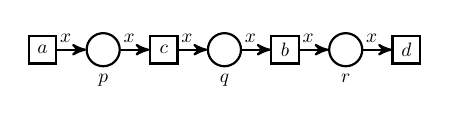
\begin{tikzpicture}[->,>=stealth',auto,x=10mm,y=1cm,node distance=11mm and 3mm,thick,  every node/.style={scale=0.7}]
			\node[tr] (a) {$a$};
			\node[pl,right of = a, label=below:$p$] (p) {};
			\node[tr,right of = p] (b) {$c$};
			\node[pl,right of = b, label=below:$q$] (q) {};
			\node[tr,right of = q] (c) {$b$};
			\node[pl,right of = c, label=below:$r$] (r) {};
			\node[tr,right of = r] (d) {$d$};
			\path[->]
				(a) edge node[above,pos=.3]{$x$} (p)
				(p) edge node[above,pos=.3]{$x$} (b)
				(b) edge node[above,pos=.3]{$x$} (q)
				(q) edge node[above,pos=.3]{$x$} (c)
				(c) edge node[above,pos=.3]{$x$} (r)
				(r) edge node[above,pos=.3]{$x$} (d);  
			\end{tikzpicture}
        \caption{\tjn $N$\label{fig:tjn-n}}
	\end{subfigure}
	\begin{subfigure}{.45\textwidth}
		\centering
		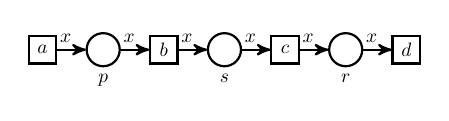
\begin{tikzpicture}[->,>=stealth',auto,x=10mm,y=1cm,node distance=11mm and 3mm,thick,  every node/.style={scale=0.7}]
			\node[tr,] (a) {$a$};
			\node[pl,right of = a, label=below:$p$] (p) {};
			\node[tr,right of = p] (b) {$b$};
			\node[pl,right of = b, label=below:$s$] (s) {};
			\node[tr,right of = s] (c) {$c$};
			\node[pl,right of = c, label=below:$r$] (r) {};
			\node[tr,right of = r] (d) {$d$};
			\path[->]
				(a) edge node[above,pos=.3]{$x$} (p)
				(p) edge node[above,pos=.3]{$x$} (b)
				(b) edge node[above,pos=.3]{$x$} (s)
				(s) edge node[above,pos=.3]{$x$} (c)
				(c) edge node[above,pos=.3]{$x$} (r)
				(r) edge node[above,pos=.3]{$x$} (d);  
			\end{tikzpicture}
        \caption{\tjn $M$\label{fig:tjn-m}}
	\end{subfigure}
	\begin{subfigure}{.6\textwidth}
		\centering
			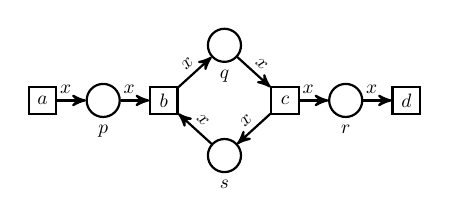
\begin{tikzpicture}[->,>=stealth',auto,x=10mm,y=1cm,node distance=11mm and 3mm,thick,  every node/.style={scale=0.7}]
			\node[tr] (a) {$a$};
			\node[pl,right of = a, label=below:$p$] (p) {};
			\node[tr,right of = p] (b) {$b$};
			\node[pl,right of = b, label=below:$s$,yshift=-1cm] (s) {};
			\node[pl,right of = b, label=below:$q$,yshift=1cm] (q) {};
			\node[tr,right of = s, yshift=1cm] (c) {$c$};
			\node[pl,right of = c, label=below:$r$] (r) {};
			\node[tr,right of = r] (d) {$d$};
			\path[->]
				(a) edge node[above,pos=.3]{$x$} (p)
				(p) edge node[above,pos=.3]{$x$} (b)
				(b) edge node[above,sloped]{$x$} (q)
				(q) edge node[above,sloped]{$x$} (c)
				(c) edge node[above,sloped]{$x$} (s)
				(s) edge node[above,sloped]{$x$} (b)
				(c) edge node[above,pos=.3]{$x$} (r)
				(r) edge node[above,pos=.3]{$x$} (d);  
			\end{tikzpicture}
        \caption{\tpnid $\compose{N}{M}$}
	\end{subfigure}
\caption{Although both $N$ and $M$ are \tjns, their composition is not}\label{fig:union-example}
\end{figure}

It is easy to see that the composition of two \tjns does not automatically result in a \tjn. Consider nets in \figref{union-example}. It is easy to see that both $N$ and $M$ can be obtained by applying \ref{itm:tjn_R2} from \defref{typed_jackson_net}. However, their composition %$\compose{N}{M}$ 
cannot be reduced to a single transition by consecutively applying rules from \defref{typed_jackson_net}.




\begin{figure}
	\centering
	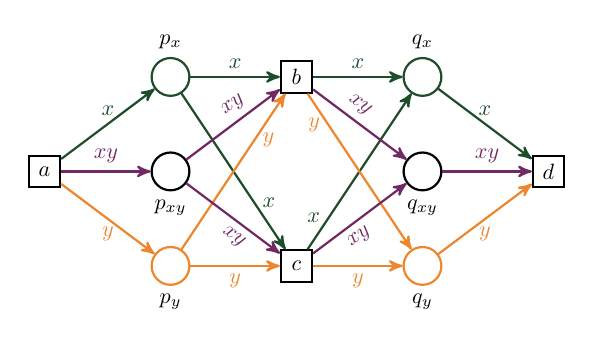
\begin{tikzpicture}[->,>=stealth',auto,node distance=20mm and 12mm,thick,  every node/.style={scale=0.8}]

\node[tr] (a) {$a$};
\node[pl,right of = a, label=above:$p_x$,yshift=15mm,green1] (px) {};
\node[pl,right of = a, label=below:$p_{xy}$] (p) {};
\node[pl,right of = a, label=below:$p_y$,yshift=-15mm,cadmiumorange] (py) {};
\node[tr, right of = px] (b) {$b$};
\node[tr, right of = py] (c) {$c$};
\node[pl,right of = b, label=above:$q_x$,green1] (qx) {};
\node[pl,right of = c, label=below:$q_y$,cadmiumorange] (qy) {};
\node[pl,right of = b, label=below:$q_{xy}$,yshift=-15mm] (q) {};
\node[tr, right of = q] (d) {$d$};


\path[->,green1]
(a) edge node[above]{$x$} (px)
(px) edge node[above]{$x$} (b)
(b) edge node[above]{$x$} (qx)
(qx) edge node[above]{$x$} (d)
(px) edge node[right, pos=.7]{$x$} (c)
(c) edge node[left, pos=.2]{$x$} (qx)
;  

\path[->,cadmiumorange]
(a) edge  node[below]{$y$} (py)
(py) edge node[below]{$y$} (c)
(py) edge node[right,pos=.7]{$y$} (b)
(b) edge node[left,pos=.2]{$y$} (qy)
(c) edge node[below]{$y$} (qy)
(qy) edge node[below]{$y$} (d)
;  


\path[->,byzantium]
(a) edge node[above]{$xy$} (p)
(p) edge node[above,sloped, pos=.6]{$xy$} (b)
(p) edge node[below,sloped, pos=.6]{$xy$} (c)
(b) edge node[above,sloped,pos=.4]{$xy$} (q)
(c) edge node[below,sloped,pos=.4]{$xy$} (q) 
(q) edge node[above]{$xy$} (d)
;  
\end{tikzpicture}
	\caption{Composition of the projections on $\set{\lambda_1}$, $\set{\lambda_2}$ and $\set{\lambda_1,\lambda_2}$ on the \tjn $(a;[p,\tup{x,y}]; (b||c);[q,\tup{x,y}];d)$. Here, type assignments are as follows: 
	$\alpha(p_x)=\alpha(q_x)=\lambda_1$,
	$\alpha(p_y)=\alpha(q_y)=\lambda_2$ and 
	$\alpha(p)=\alpha(q)=\lambda_1\lambda_2$.}
	\label{fig:proj-union-example}
\end{figure}


A more surprising observation is that composing type projections of a \tjn may not result in a \tjn. Take for example the net from Figure~\ref{fig:proj-union-example}. 
Both its projections on $\set{\lambda_1}$ and $\set{\lambda_2}$ are \tjns. 
However, bringing them together using the composition operator results in a \tpnid that is not \tjn: indeed, since the ``copies'' of place $p$ appear in three places, and all such copies have same pre- and post-sets (and only differ by their respective types), it is impossible to apply identifier elimination rule \emph{R6} from \defref{typed_jackson_net}.

As one may observe from the above example, 
the only difference between $[p_{xy},\tup{\lambda_1,\lambda_2}]$ and its copies $p_x$ and $p_y$ is in their respective types, whereas the identifiers carried by $p_x$ and $p_y$ are always contained in $p_{xy}$, and thus both $p_x$ and $p_y$ can be seen as subsidiary with respect to $p_{xy}$. 
We formalize this observation using the notion of \emph{minor places}:  
a place $p$ is minor to some place $q$ if both $p$ and $q$ have identical pre- and post-sets, and the type of $q$ subsumes the one of $p$. 


\begin{definition}[Minor places] \deflabel{minor_places}
Let $N = (P_N, T_N, F_N, \alpha, \beta)$ be a \tpnid.
A place $p\in P$ is \emph{minor to} a place $q\in P$ iff the following holds:
\begin{compactitem}
\item  $\pre{p}=\pre{q}$, $\post{p}=\post{q}$ and $\alpha(p)\subset \alpha(q)$; 
\item  $\beta((t,p))=\restr{\beta((t,q))}{\type^{-1}(\alpha(p))}$, for each $t\in\pre{p}$;
\item  $\beta((p,t))=\restr{\beta((q,t))}{\type^{-1}(\alpha(p))}$, for each $t\in\post{p}$.
\end{compactitem}
\end{definition}

We show next that minor places can be added or removed without altering the overall behavior of the net.

\begin{lemma}
\label{lemma:minors}
Let $N = (P, T, F, \alpha, \beta)$ be a \tpnid with initial marking $m_0$ s.t. 
$m_0(p)=m_0(q)=\emptyset$, for $p,q\in P$, where $p$ is minor to $q$.
Let $N'=(P\setminus\set{p}, T, F\setminus(\set{(p,t)|t\in\post{p}}\cup\set{(t,p)|t\in\pre{p}}),\alpha,\beta)$ be a \tpnid obtained by eliminating from $N$ place $p$ .
Then $\transitionsystem{N,m_0}\sim^r \transitionsystem{N',m_0}$.
\end{lemma}
%\andy{we need to define bisimulation of two \tpnids}
\begin{proof}(sketch)
It is enough to define a relation $Q\subseteq \pnreachable{N}{m_0}\times \pnreachable{N'}{m_0}$ s.t. $(m,m')\in Q$ iff $m(r)=m'(r)$, for $r\in P\setminus\set{p}$, and $m(p)(\cname{id})=m'(q)(\cname{id})$, for all $\cname{id}\in\colset(\place)$, and $|m(p)|=|m'(q)|$.
Then the lemma statement directly follows from the firing rule of \tpnids and that pre- and post-sets of $p$ and $q$ coincide.
\end{proof}

\begin{figure}[t!]
  \centering
	\begin{subfigure}{.38\textwidth}
		\centering
		 	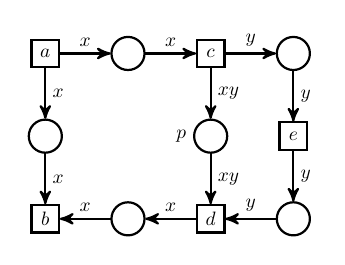
\begin{tikzpicture}[->,>=stealth',auto,x=10mm,y=1cm,node distance=15mm and 3mm,thick,  every node/.style={scale=0.7}]
			\node[tr] (a) {$a$};
			\node[pl,right of = a] (p1) {};
			\node[tr,right of = p1] (c) {$c$};			
			\node[pl,right of = c] (p5){};
			\node[tr,below of = p5] (e){$e$};
			 \node[pl,below of = e] (p6){};
			\node[pl,below of = a] (p2) {};
			\node[tr,below of = p2] (b){$b$};
			\node[pl,below of = c,label=left:$p$] (p3) {};
			\node[tr,below of = p3] (d) {$d$};
			\node[pl, left of = d] (p4){};
			\path[->]
				(a) edge node[above]{$x$} (p1)
				(a) edge node[right]{$x$} (p2)
				(p1) edge node[above]{$x$} (c)
				(p2) edge node[right]{$x$} (b)
				(p4) edge node[above]{$x$} (b)
				(d) edge node[above]{$x$}  (p4)
				(c) edge node[right]{$xy$} (p3)
				(p3) edge node[right]{$xy$}  (d)
				(c) edge node[above]{$y$}  (p5)
				(p5) edge node[right]{$y$} (e)
				(e) edge node[right]{$y$} (p6)
				(p6) edge node[above]{$y$} (d);  
			\end{tikzpicture}
        \caption{\tpnid $N$ with $\type(x)=\lambda_1$ and $\type(y)=\lambda_2$\label{fig:singleton-tjn-n}}
	\end{subfigure}
	\begin{subfigure}{.3\textwidth}
		\centering
		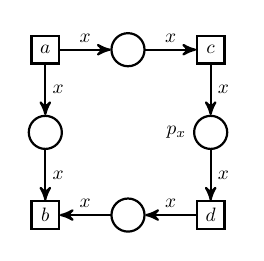
\begin{tikzpicture}[->,>=stealth',auto,x=10mm,y=1cm,node distance=15mm and 3mm,thick,  every node/.style={scale=0.7}]
			\node[tr] (a) {$a$};
			\node[pl,right of = a] (p1) {};
			\node[tr,right of = p1] (c) {$c$};			
			\node[pl,below of = a] (p2) {};
			\node[tr,below of = p2] (b){$b$};
			\node[pl,below of = c,label=left:$p_x$] (p3) {};
			\node[tr,below of = p3] (d) {$d$};
			\node[pl, left of = d] (p4){};
			\path[->]
				(a) edge node[above]{$x$} (p1)
				(a) edge node[right]{$x$} (p2)
				(p1) edge node[above]{$x$} (c)
				(p2) edge node[right]{$x$} (b)
				(p4) edge node[above]{$x$} (b)
				(d) edge node[above]{$x$}  (p4)
				(c) edge node[right]{$x$} (p3)
				(p3) edge node[right]{$x$}  (d);
			\end{tikzpicture}
        \caption{The projection of $\set{\lambda_1}$ on $N$ \label{fig:singleton-tjn-m}}
	\end{subfigure}
	\begin{subfigure}{.3\textwidth}
		\centering
		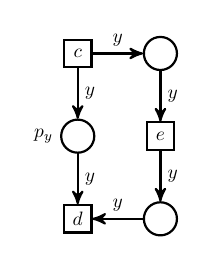
\begin{tikzpicture}[->,>=stealth',auto,x=10mm,y=1cm,node distance=15mm and 3mm,thick,  every node/.style={scale=0.7}]
			\node[tr] (c) {$c$};			
			\node[pl,right of = c] (p5){};
			\node[tr,below of = p5] (e){$e$};
			 \node[pl,below of = e] (p6){};
			\node[pl,below of = c,label=left:$p_y$] (p3) {};
			\node[tr,below of = p3] (d) {$d$};
			\path[->]
				(c) edge node[right]{$y$} (p3)
				(p3) edge node[right]{$y$}  (d)
				(c) edge node[above]{$y$}  (p5)
				(p5) edge node[right]{$y$} (e)
				(e) edge node[right]{$y$} (p6)
				(p6) edge node[above]{$y$} (d);  
			\end{tikzpicture}
        \caption{The projection of $\set{\lambda_2}$ on $N$ \label{fig:singleton-tjn-k}}
	\end{subfigure}
	\begin{subfigure}{.7\textwidth}
		\centering
		 	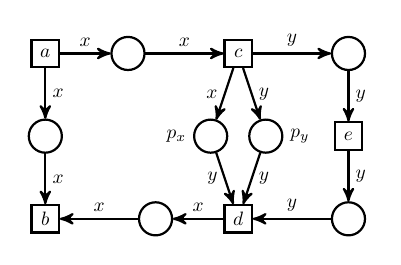
\begin{tikzpicture}[->,>=stealth',auto,x=10mm,y=1cm,node distance=15mm and 3mm,thick,  every node/.style={scale=0.7}]
			\node[tr] (a) {$a$};
			\node[pl,right of = a] (p1) {};
			\node[tr,right of = p1,xshift=5mm] (c) {$c$};			
			\node[pl,right of = c,xshift=5mm] (p5){};
			\node[tr,below of = p5] (e){$e$};
			 \node[pl,below of = e] (p6){};
			\node[pl,below of = a] (p2) {};
			\node[tr,below of = p2] (b){$b$};
			\node[pl,below of = c,label=left:$p_x$,xshift=-.5cm] (px) {};
			\node[pl,below of = c,label=right:$p_y$,xshift=.5cm] (py) {};

			\node[tr,below of = px,xshift=.5cm] (d) {$d$};
			\node[pl, left of = d] (p4){};
			\path[->]
				(a) edge node[above]{$x$} (p1)
				(a) edge node[right]{$x$} (p2)
				(p1) edge node[above]{$x$} (c)
				(p2) edge node[right]{$x$} (b)
				(p4) edge node[above]{$x$} (b)
				(d) edge node[above]{$x$}  (p4)
				(c) edge node[left]{$x$} (px)
				(px) edge node[left]{$y$}  (d)
				(c) edge node[right]{$y$} (py)
				(py) edge node[right]{$y$}  (d)
				(c) edge node[above]{$y$}  (p5)
				(p5) edge node[right]{$y$} (e)
				(e) edge node[right]{$y$} (p6)
				(p6) edge node[above]{$y$} (d);  
			\end{tikzpicture}
        \caption{The composition of  $\project{\set{\lambda_1}}{N}$ and $\project{\set{\lambda_2}}{N}$\label{fig:compose-singleton}}
	\end{subfigure}
\caption{\tpnid $N$ (\ref{fig:singleton-tjn-n}), its singleton projections  and their composition }\label{fig:singleton-example}
\end{figure}

Let us now address the reconstructability property.
In a nutshell, a net is reconstructable if composing all of its type projections 
returns the same net. 
This property is not that trivial to obtain.
For example, let us consider singleton projections (that is, projections $\project{\set{\lambda}}{N}$ obtained for each $\lambda\in\type_\Lambda(N)$)
of the net in \figref{singleton-example}.
It is easy to see that such projections ``ignore'' interactions between objects (or system components).
Thus, the composition of the singleton projections $\project{\set{\lambda_1}}{N}$ and $\project{\set{\lambda_2}}{N}$ from \figref{singleton-example} does not result in a model
that merges $p_x$ and $p_y$ in one place as the composition operator cannot recognize component interactions between such projections. 
This is reflected in \figref{compose-singleton}.





To be able to reconstruct the original model from its projections (or at least do it approximately well), 
one needs to consider a projection reflecting component interactions. In the case of the net from Figure~\ref{fig:singleton-tjn-n}, its non-singleton projection $\project{\set{\lambda_1,\lambda_2}}{N}$ is depicted in Figure~\ref{fig:interactions-n}.
Now, using this projection we can obtain a composition (see Figure~\ref{fig:compose-full}) that closely resembles $N$. 
Notice that, in this composition, copies of the interaction place $p$ appear three times as places $p_x$, $p_y$ and $p_{xy}$, respectively.
It is also easy to see that places $p_x$ and $p_y$ are minor to $p_{xy}$, and 
$\alpha(p)=\alpha(p_{xy})$ witnesses that $\project{\set{\lambda_1,\lambda_2}}{N}$ is the maximal projection defined over types of $N$ s.t. the correct type of $p$ is ``reconstructed''.
This leads us to the following result stipulating the reconstructability property of typed Jackson nets. 


\begin{figure}[t!]
  \centering
	\begin{subfigure}{.4\textwidth}
		\centering
		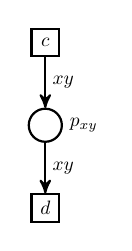
\begin{tikzpicture}[->,>=stealth',auto,x=10mm,y=1cm,node distance=15mm and 3mm,thick,  every node/.style={scale=0.7}]
			\node[tr] (c) {$c$};			
			 \node[pl,below of = c,label=right:$p_{xy}$] (p){};
			\node[tr,below of = p] (d) {$d$};
			\path[->]
				(c) edge node[right]{$xy$} (p)
				(p) edge node[right]{$xy$} (d);  
			\end{tikzpicture}
        \caption{The projection of $\set{\lambda_1,\lambda_2}$ on $N$ from Figure~\ref{fig:singleton-tjn-n} \label{fig:interactions-n}}
	\end{subfigure}\quad
	\begin{subfigure}{.5\textwidth}
		\centering
		 	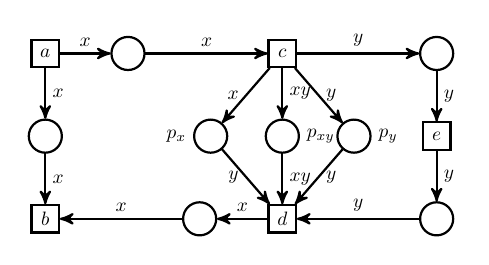
\begin{tikzpicture}[->,>=stealth',auto,x=10mm,y=1cm,node distance=15mm and 3mm,thick,  every node/.style={scale=0.7}]
			\node[tr] (a) {$a$};
			\node[pl,right of = a] (p1) {};
			\node[tr,right of = p1,xshift=13mm] (c) {$c$};			
			\node[pl,right of = c,xshift=13mm] (p5){};
			\node[tr,below of = p5] (e){$e$};
			 \node[pl,below of = e] (p6){};
			\node[pl,below of = a] (p2) {};
			\node[tr,below of = p2] (b){$b$};
			\node[pl,below of = c,label=left:$p_x$,xshift=-13mm] (px) {};
			\node[pl,below of = c,label=right:$p_y$,xshift=13mm] (py) {};
			\node[pl,below of = c,label=right:$p_{xy}$] (p) {};

			\node[tr,below of = px,xshift=13mm] (d) {$d$};
			\node[pl, left of = d] (p4){};
			\path[->]
				(a) edge node[above]{$x$} (p1)
				(a) edge node[right]{$x$} (p2)
				(p1) edge node[above]{$x$} (c)
				(p2) edge node[right]{$x$} (b)
				(p4) edge node[above]{$x$} (b)
				(d) edge node[above]{$x$}  (p4)
				(c) edge node[left]{$x$} (px)
				(px) edge node[left]{$y$}  (d)
				(c) edge node[right]{$xy$} (p)
				(p) edge node[right]{$xy$}  (d)
				(c) edge node[right]{$y$} (py)
				(py) edge node[right]{$y$}  (d)
				(c) edge node[above]{$y$}  (p5)
				(p5) edge node[right]{$y$} (e)
				(e) edge node[right]{$y$} (p6)
				(p6) edge node[above]{$y$} (d);  
			\end{tikzpicture}
			  \caption{The composition  $\project{\set{\lambda_1}}{N}\composeOperator\project{\set{\lambda_2}}{N}\composeOperator\project{\set{\lambda_1,\lambda_2}}{N}$  for $N$ from Figure~\ref{fig:singleton-tjn-n} \label{fig:compose-full}}
%        \caption{The composition  $\biguplus\limits_{\Upsilon\subseteq\type_\Lambda(N)}\project{\Upsilon}{N}$ for $N$ from Figure~\ref{fig:singleton-tjn-n} \label{fig:compose-full}}
	\end{subfigure}
\caption{Adding the projection $\project{\set{\lambda_1,\lambda_2}}{N}$ reflecting interactions to the composition results in the original net $N$ modulo places minor to $p$ (such as $p_x$ and $p_y$). }\label{fig:compose-interactions}
\end{figure}

\begin{theorem}\thmlabel{reconstructability}
Let $N = (P, T, F, \alpha, \beta)$ be a \tjn. 
Then $\transitionsystem{N,\emptyset}\sim^r \transitionsystem{N',\emptyset}$, where\\ $N'=\biguplus\limits_{\emptyset\subset\Upsilon\subseteq\type_\Lambda(N)}\project{\Upsilon}{N}$. 
\end{theorem}
\begin{proof} (sketch)
The proof immediately follows from the next observation.
Among all possible projections, for each place $p\in P$ there exists a projection $\project{\Upsilon}{N}$ such that $\alpha(p)=\Upsilon$. This also means that $\project{\Upsilon}{N}$ contains $p$ and that all other projections $\project{\Upsilon'}{N}$ with $\Upsilon'\subset\Upsilon$ will at most include the minors of $p$. 
Following \defref{composition}, it is easy to see that the composition of all the projections yields a \tjn identical to $N$ modulo additional place minors introduced by some of the projections. Showing that the obtained net is bisimilar to $N$ can be done by analogy with Lemma~\ref{lemma:minors}.
\end{proof}

	
Notice that the above result can be made stronger if all the additional minors (i.e., minors that were not present originally in $N$) are removed using reduction rules from \defref{typed_jackson_net}. For simplicity, given a \tpnid $N$ with the set of places $P$, we denote by $\lfloor P \rfloor$ the set of its minor places. 

\begin{corollary}\corlabel{reconstructability}
Let $N$ be a \tjn and $N'$ is as in \thmref{reconstructability}. 
Then $(N,\emptyset)\leftrightsquigarrow(N',\emptyset)$, if $\lfloor P \rfloor = \lfloor P' \rfloor$, where $P$ and $P'$ are respectively the sets of places of $N$ and $N'$.
\end{corollary}
The above result can be obtained by complementing the proof of \thmref{reconstructability} with a step that applies finitely many \tjn reduction rules to all the minor places that are in $N'$ and not in $N$.

\endinput


\begin{property} \proplabel{composition_gives_tjn}
	Let $N = (P, T, F, \alpha, \beta)$ a \tjn, and suppose $N_\gamma = \project{\gamma}{N}$ and $N_\delta = \project{\delta}{N}$ two projections. Then their composition $\compose{N_\gamma}{N_\delta}$ is a \tjn.
\end{property}

\begin{proof} \prflabel{composition_gives_tjn}
	This proofs \propref{composition_gives_tjn}.
\end{proof}


\andy{elaborate more on this property: simply say that behavioral correlations between types are not enough and demonstrate that on a simple example with two subnets for types x and xyz}
\begin{property} \proplabel{projection_not_simulated}
	Let $N = (P, T, F, \alpha, \beta)$ a \tpnid, and $\lambda, \gamma \in \Lambda$ two types such that $\lambda \subseteq \gamma$.
	Then the type projection on $\lambda$ is not simulated by the type projection on $\gamma$, that is, $\delaysim{\project{\lambda}{N}}{}{\project{\gamma}{N}}$ does not hold.
\end{property}

\begin{proof} \prflabel{projection_not_simulated}
	This proofs \propref{projection_not_simulated} by counterexample, see whiteboard.
\end{proof}

\begin{definition}[Projection closure] \deflabel{projection_closure}
	Let $\lambda \in \Lambda$ be a type. Given a \tpnid $N = (P_N, T_N, F_N, \alpha, \beta)$, its \emph{closed $\lambda$-projection} $\projectClosure{\lambda}{N} = (P, T, F, \alpha, \beta)$ is a \tpnid with
	\begin{compactitem}
		\item $P = \set{p \in P_N \mid \alpha(p) \subseteq \lambda}$
		\item $T = \set{t \in T_N \mid ({}_N^\bullet t \cup t^\bullet_N) \cap P \neq \emptyset}$, \dbtodo{are these presets and postsets defined somewhere?}
		\item $F = F_N \cap ((P \times T) \cup (T \times P))$
	\end{compactitem}
\end{definition}

\begin{corollary} \corlabel{closure_projection_is_itself}
	The closed projection over all $\Lambda$ for \tpnid $N$ is  isomorphic equivalent to $N$:
	$$
	\projectClosure{\Lambda}{N} = N
	$$
\end{corollary}

\begin{proof} \deflabel{closure_projection_is_itself}
	This proofs \corref{closure_projection_is_itself}.
\end{proof}

\begin{theorem} \thmlabel{decomposability}
	Let $N = (P, T, F, \alpha, \beta)$ a \tpnid, and $\gamma \subseteq \Lambda$ a set of types. Then the following holds.
	$$
	\Composed{\lambda \in \gamma^*}  \strongbisim{\project{\lambda}{N}}{}{\projectClosure{\gamma}{N}}
	$$
\end{theorem}

\begin{proof} \prflabel{decomposability}
	This proofs \thmref{decomposability}.
\end{proof}


\begin{corollary} \corlabel{decomposability}
	Let $N = (P, T, F, \alpha, \beta)$ a \tjn, then the following holds.
	$$
	\Composed{\lambda \in \Lambda^*} \project{\lambda}{N} = N
	$$
\end{corollary}

\begin{proof} \prflabel{arg1}
	Follows directly from \correffull{closure_projection_is_itself} and \thmreffull{decomposability}.
\end{proof}
%
%
%\begin{property} \proplabel{composition_gives_tjn}
%	Let $N = (P, T, F, \alpha, \beta)$ a \tjn, and suppose $N_\gamma = \project{\gamma}{N}$ and $N_\delta = \project{\delta}{N}$ two projections. Then their composition $\compose{N_\gamma}{N_\delta}$ is a \tjn.
%\end{property}
%
%\begin{proof} \prflabel{composition_gives_tjn}
%	This proofs \propref{composition_gives_tjn}.
%\end{proof}
%
%
%\andy{elaborate more on this property: simply say that behavioral correlations between types are not enough and demonstrate that on a simple example with two subnets for types x and xyz}
%\begin{property} \proplabel{projection_not_simulated}
%	Let $N = (P, T, F, \alpha, \beta)$ a \tpnid, and $\lambda, \gamma \in \Lambda$ two types such that $\lambda \subseteq \gamma$.
%	Then the type projection on $\lambda$ is not simulated by the type projection on $\gamma$, that is, $\delaysim{\project{\lambda}{N}}{}{\project{\gamma}{N}}$ does not hold.
%\end{property}
%
%\begin{proof} \prflabel{projection_not_simulated}
%	This proofs \propref{projection_not_simulated} by counterexample, see whiteboard.
%\end{proof}
%
%\begin{definition}[Projection closure] \deflabel{projection_closure}
%	Let $\lambda \in \Lambda$ be a type. Given a \tpnid $N = (P_N, T_N, F_N, \alpha, \beta)$, its \emph{closed $\lambda$-projection} $\projectClosure{\lambda}{N} = (P, T, F, \alpha, \beta)$ is a \tpnid with
%	\begin{compactitem}
%		\item $P = \set{p \in P_N \mid \alpha(p) \subseteq \lambda}$
%		\item $T = \set{t \in T_N \mid ({}_N^\bullet t \cup t^\bullet_N) \cap P \neq \emptyset}$, \dbtodo{are these presets and postsets defined somewhere?}
%		\item $F = F_N \cap ((P \times T) \cup (T \times P))$
%	\end{compactitem}
%\end{definition}
%
%\begin{corollary} \corlabel{closure_projection_is_itself}
%	The closed projection over all $\Lambda$ for \tpnid $N$ is  isomorphic equivalent to $N$:
%	$$
%	\projectClosure{\Lambda}{N} = N
%	$$
%\end{corollary}
%
%\begin{proof} \deflabel{closure_projection_is_itself}
%	This proofs \corref{closure_projection_is_itself}.
%\end{proof}
%
%\begin{theorem} \thmlabel{decomposability}
%	Let $N = (P, T, F, \alpha, \beta)$ a \tpnid, and $\gamma \subseteq \Lambda$ a set of types. Then the following holds.
%	$$
%	\Composed{\lambda \in \gamma^*}  \strongbisim{\project{\lambda}{N}}{}{\projectClosure{\gamma}{N}}
%	$$
%\end{theorem}
%
%\begin{proof} \prflabel{decomposability}
%	This proofs \thmref{decomposability}.
%\end{proof}
%
%
%\begin{corollary} \corlabel{decomposability}
%	Let $N = (P, T, F, \alpha, \beta)$ a \tjn, then the following holds.
%	$$
%	\Composed{\lambda \in \Lambda^*} \project{\lambda}{N} = N
%	$$
%\end{corollary}
%
%\begin{proof} \prflabel{arg1}
%	Follows directly from \correffull{closure_projection_is_itself} and \thmreffull{decomposability}.
%\end{proof}
>>>>>>> 1cae204e8fc233fb1cd2f50e31b7b50be10dbbf6


%
%% everything below here is old
%
%
%For the sake of simplicity, we make the following assumption:\andy{elaborate more on this assumption}
%%Note tha\\t from \defref{typed_jackson_nets} it follows that transitions have unique actions, and can thus be identified precisely..
%\begin{assumption}
%	\tjns have unique transition labels; \db{No longer necessary I think, since we can just state that $\ell$ maps to unique actions, and there is a bijection between \A and $\Lambda$}.
%\end{assumption}
%
%
%\begin{figure}
%	\centering
%	\includegraphics[width=\linewidth]{figs/screenshot_extended_paper_definition_projection}
%	\caption{\dbtodo{Definition of type projection is needed.}}
%	\label{fig:screenshotextendedpaperdefinitionprojection}
%\end{figure}
%
%
%Now, we define a full t-JN decomposition. In the nutshell, the full decomposition is a set of t-JNs obtained from the original one by constructing named projections for every inscription in the original net.
%
%\begin{definition}[Full decomposition]
%	Idea: given a t-JN $N$, build a set $dec(N)$ consisting of named projections, where a each projection is obtained for a set take from one of the net inscriptions.
%	\andy{add the definition (has to be constructive, algorithm-like)}
%\end{definition}
%
%COMPOSITION OPERATOR
%
%Now, we introduce a special operator that, given two t-JNs, puts them into a synchronous composition, where the synchronization is realized only for same-labeled transitions.
%We start with an example explaining the idea behind this operator.
%
%\begin{example}
%	\label{ex:tjn-projections}
%	\andy{rewrite/complete the example + show which rules are used to construct the original net $N$}
%	Consider the following typed t-JN $N$.
%	\begin{center}
%		\begin{tikzpicture}[->,>=stealth',auto,x=15mm,y=1.0cm,node distance=15mm and 7mm,thick, scale=0.8, every node/.style={scale=0.8}]
%
%			\node[tr] (a) {$a$};
%			\node[pl,right of = a] (p1) {};
%			\node[tr, right of = p1] (b) {$b$};
%			\node[tr, below of = p1] (c) {$c$};
%			\node[pl,right of = c] (p2) {};
%			\node[tr,right of = p2] (d) {$d$};
%			\node[pl,right of = d] (p3) {};
%			\node[tr,right of = p3] (f) {$f$};
%			\node[pl,below of = p2,yshift=4mm] (p4){};
%			\node[tr,right of = p4] (e) {$e$};
%			\node[pl,right of = e] (p5) {};
%			\node[pl,below of = p4,yshift=4mm] (p6){};
%			\node[tr,right of = p6] (g) {$g$};
%			\node[pl,right of = g] (p7) {};
%
%
%
%			\path[->]
%			(a) edge node{$x$} (p1)
%			(p1) edge node{$x$} (b)
%			(p1) edge node{$x$} (c)
%			(c) edge node{$xyz$} (p2)
%			(p2)  edge node{$xyz$} (d)
%			(d) edge node{$xyz$} (p3)
%			(p3) edge node{$xyz$}  (f)
%			(f.north) edge[above,in=-30,out=150] node{$x$} (p1)
%			(c)  edge[above,bend right=10] node{$y$} (p4)
%			(p4) edge node{$y$} (e)
%			(e)  edge node{$y$} (p5)
%			(p5) edge[above,bend right=10] node{$y$} (f)
%			(c.south) edge[above,bend right=20] node{$z$}  (p6)
%			(p6) edge[above] node{$z$} (g)
%			(g) edge[above] node{$z$} (p7)
%			(p7) edge[above,bend right=20] node{$z$} (f.south)
%			;
%		\end{tikzpicture}
%	\end{center}
%
%	For the above net, we construct the following named projections.
%	\begin{enumerate}
%		\item For $X=\set{x}$, we get the following net:
%		      \begin{center}
%			      \begin{tikzpicture}[->,>=stealth',auto,x=15mm,y=1.0cm,node distance=15mm and 7mm,thick,scale=0.8, every node/.style={scale=0.8}]
%				      \node[tr] (a) {$a$};
%				      \node[pl,right of = a] (p1) {};
%				      \node[tr, right of = p1] (b) {$b$};
%				      \node[tr, below of = p1] (c) {$c$};
%				      \node[pl,right of = c] (p2) {};
%				      \node[tr,right of = p2] (d) {$d$};
%				      \node[pl,right of = d] (p3) {};
%				      \node[tr,right of = p3] (f) {$f$};
%				      \path[->]
%				      (a) edge node{$x$} (p1)
%				      (p1) edge node{$x$} (b)
%				      (p1) edge node{$x$} (c)
%				      (c) edge node{$x$} (p2)
%				      (p2)  edge node{$x$} (d)
%				      (d) edge node{$x$} (p3)
%				      (p3) edge node{$x$}  (f)
%				      (f.north) edge[above,in=-30,out=150] node{$x$} (p1);
%			      \end{tikzpicture}
%		      \end{center}
%		\item For $X=\set{y}$, we get the following net:
%		      \begin{center}
%			      \begin{tikzpicture}[->,>=stealth',auto,x=15mm,y=1.0cm,node distance=15mm and 7mm,thick,scale=0.8, every node/.style={scale=0.8}]
%				      \node[tr] (c) {$c$};
%				      \node[pl,right of = c] (p2) {};
%				      \node[tr,right of = p2] (d) {$d$};
%				      \node[pl,right of = d] (p3) {};
%				      \node[tr,right of = p3] (f) {$f$};
%				      \node[pl,below of = p2,yshift=4mm] (p4){};
%				      \node[tr,right of = p4] (e) {$e$};
%				      \node[pl,right of = e] (p5) {};
%				      \path[->]
%				      (c) edge node{$y$} (p2)
%				      (p2)  edge node{$y$} (d)
%				      (d) edge node{$y$} (p3)
%				      (p3) edge node{$y$}  (f)
%				      (c)  edge[above,bend right=10] node{$y$} (p4)
%				      (p4) edge node{$y$} (e)
%				      (e)  edge node{$y$} (p5)
%				      (p5) edge[above,bend right=10] node{$y$} (f);
%			      \end{tikzpicture}
%		      \end{center}
%		\item For $X=\set{z}$, we get the following net:
%		      \begin{center}
%			      \begin{tikzpicture}[->,>=stealth',auto,x=15mm,y=1.0cm,node distance=15mm and 7mm,thick,scale=0.8, every node/.style={scale=0.8}]
%				      \node[tr] (c) {$c$};
%				      \node[pl,right of = c] (p2) {};
%				      \node[tr,right of = p2] (d) {$d$};
%				      \node[pl,right of = d] (p3) {};
%				      \node[tr,right of = p3] (f) {$f$};
%				      \node[pl,below of = p2,yshift=4mm] (p4){};
%				      \node[tr,right of = p4] (e) {$g$};
%				      \node[pl,right of = e] (p5) {};
%				      \path[->]
%				      (c) edge node{$z$} (p2)
%				      (p2)  edge node{$z$} (d)
%				      (d) edge node{$z$} (p3)
%				      (p3) edge node{$z$}  (f)
%				      (c)  edge[above,bend right=10] node{$z$} (p4)
%				      (p4) edge node{$z$} (e)
%				      (e)  edge node{$z$} (p5)
%				      (p5) edge[above,bend right=10] node{$z$} (f);
%			      \end{tikzpicture}
%		      \end{center}
%		\item Finally, for $X=\set{x,y,z}$, we obtain the following t-JN:
%		      \begin{center}
%			      \begin{tikzpicture}[->,>=stealth',auto,x=15mm,y=1.0cm,node distance=15mm and 7mm,thick,scale=0.8, every node/.style={scale=0.8}]
%				      \node[tr] (c) {$c$};
%				      \node[pl,right of = c] (p2) {};
%				      \node[tr,right of = p2] (d) {$d$};
%				      \node[pl,right of = d] (p3) {};
%				      \node[tr,right of = p3] (f) {$f$};
%				      \path[->]
%				      (c) edge node{$xyz$} (p2)
%				      (p2)  edge node{$xyz$} (d)
%				      (d) edge node{$xyz$} (p3)
%				      (p3) edge node{$xyz$}  (f);
%			      \end{tikzpicture}
%		      \end{center}
%	\end{enumerate}
%
%	Now, we would like to see how to merge the obtained projections. By simply juxtaposing the above projections, we  obtain the following net:
%
%	\begin{center}
%		\begin{tikzpicture}[->,>=stealth',auto,x=15mm,y=1.0cm,node distance=15mm and 7mm,thick, scale=0.8, every node/.style={scale=0.8}]
%
%			\node[tr] (a) {$a$};
%			\node[pl,right of = a] (p1) {};
%			\node[tr, right of = p1] (b) {$b$};
%			\node[tr, below of = p1, yshift=-2cm] (c) {$c$};
%			\node[pl,right of = c,xshift=.5cm] (p2) {};
%			\node[pl,above of = p2,yshift=-6mm] (p2x) {};
%			\node[pl,below of = p2,yshift=6mm] (p2z) {};
%			\node[pl,above of = p2x,yshift=-6mm] (p2y) {};
%			\node[tr,right of = p2,xshift=.5cm] (d) {$d$};
%			\node[pl,right of = d,xshift=.5cm] (p3) {};
%			\node[tr,right of = p3,xshift=.5cm] (f) {$f$};
%			\node[pl,above of = p3,yshift=-6mm] (p3x) {};
%			\node[pl,above of = p3x,yshift=-6mm] (p3y) {};
%			\node[pl,below of = p3,yshift=6mm] (p3z) {};
%			\node[pl,below of = p2,yshift=-4mm] (p4){};
%			\node[tr,right of = p4,xshift=.5cm] (e) {$e$};
%			\node[pl,right of = e,xshift=.5cm] (p5) {};
%			\node[pl,below of = p4,yshift=4mm] (p6){};
%			\node[tr,right of = p6,xshift=.5cm] (g) {$g$};
%			\node[pl,right of = g,xshift=.5cm] (p7) {};
%
%			\path[->]
%			(a) edge node{$x$} (p1)
%			(p1) edge node{$x$} (b)
%			(p1) edge[left] node{$x$} (c)
%			(c) edge[above] node{$xyz$} (p2)
%			(p2)  edge[above] node{$xyz$} (d)
%			(d) edge[above] node{$xyz$} (p3)
%			(p3) edge[above] node{$xyz$}  (f)
%			(f.north) edge[above,in=-25,out=90] node{$x$} (p1)
%			(c)  edge[above,bend right=30,pos=.7] node{$y$} (p4)
%			(p4) edge node{$y$} (e)
%			(e)  edge node{$y$} (p5)
%			(p5) edge[above,bend right=30,pos=.2] node{$y$} (f)
%			(c.south) edge[above,bend right=20,pos=.8] node{$z$}  (p6)
%			(p6) edge[above] node{$z$} (g)
%			(g) edge[above] node{$z$} (p7)
%			(p7) edge[above,bend right=20,pos=.2] node{$z$} (f.south)
%			;
%
%			\path[->,red!60]
%			(c.north) edge[above,bend left=15] node{$x$} (p2x)
%			(p2x) edge[above,bend left=15] node{$x$} (d.north)
%			(d.north) edge[above,bend left=15] node{$x$} (p3x)
%			(p3x) edge[above,bend left=15] node{$x$} (f.north)
%			;
%
%			\path[->,blue!60]
%			(c.north) edge[above,bend left=25] node{$y$} (p2y)
%			(p2y) edge[above,bend left=25] node{$y$} (d.north)
%			(d.north) edge[above,bend left=25] node{$y$} (p3y)
%			(p3y) edge[above,bend left=25] node{$y$} (f.north)
%			;
%
%			\path[->,violet!60]
%			(c.south) edge[above,bend right=15] node{$z$} (p2z)
%			(p2z) edge[above,bend right=15] node{$z$} (d.south)
%			(d.south) edge[above,bend right=15] node{$z$} (p3z)
%			(p3z) edge[above,bend right=15] node{$z$} (f.south)
%			;
%		\end{tikzpicture}
%	\end{center}
%
%	\andy{\textbf{describe the merge here!}}
%\end{example}
%
%The above example gives an intuition of how the composition operator works for t-JNs that have a few same-labeled transitions in common. Next we formally define this operator.
%
%% %The above example gives an intuition of how the merge should not be performed in cases when typed nets with potentially partially shared identifier types are brought together. Instead, we propose the merge operator $\oplus$ that resolves the above issue. 
%% %In the nutshell, this operator creates a parallel composition of the discovered behaviors and, in case juxtaposed nets have overlapping subnets (that are not represented by single transitions), chooses the subnet that puts in relation more object types. 
%
%\begin{definition}[Synchronous product????]
%	The composition of two t-JNs $N_1 = (\places_1, \transitions_1, \flow_1, \alpha_1, \beta_1,\ell_1)$ and $N_2 = (\places_2, \transitions_2, \flow_2, \alpha_2, \beta_2,\ell_2)$ is a t-JN $N_1\oplus N_2= (\places, \transitions, \flow, \alpha, \beta,\ell)$, where:
%	\begin{itemize}
%		\item \andy{complete the definition, use the old definition as the basis}
%	\end{itemize}
%\end{definition}
%
%% %%%%%%%
%% %% OLD DEFINITION OF COMPOSITION 
%% %%%%%%%
%% %\begin{definition}
%% %The synchronous composition of two t-JNs $N_1 = (\places_1, \transitions_1, \flow_1, \alpha_1, \beta_1,\ell_1)$ and $N_2 = (\places_2, \transitions_2, \flow_2, \alpha_2, \beta_2,\ell_2)$ is a t-JN $N_1\oplus N_2= (\places, \transitions, \flow, \alpha, \beta,\ell)$, where:
%% %\begin{itemize}
%% %\item $\places= \set{p\in\places_1 \mid \not\exists p'\in\places_2,t\in \transitions_1,t'\in\transitions_2:\beta_1(p,t)\subset\beta_2(p',t') \land \ell_1(t)=\ell_2(t')}
%% %\cup \set{p\in\places_2 \mid \not\exists p'\in\places_1,t\in \transitions_2,t'\in\transitions_1:\beta_2(p,t)\subset\beta_1(p',t') \land \ell_2(t)=\ell_1(t')}$
%% %	\item $\transitions=\set{(t_1,t_2)\in \transitions_1\times \transitions_2\mid \ell_1(t_1)=\ell_2(t_2)}$
%% %	\item $\flow=\set{(p,(t_1,t_2))\in \places\times\transitions \mid (p,t_1)\in \flow_1 \text{ or }  (p,t_2)\in \flow_2} \cup \set{((t_1,t_2),p)\in \transitions\times\places \mid (t_1,p)\in \flow_1 \text{ or } (t_2,p)\in \flow_2}$ 
%% %	\item $\alpha(p)=\begin{cases} \alpha_1(p), & \text{ if }p\in\places_1 \\ \alpha_2(p), & \text{ if }p\in\places_2\end{cases}$
%% %	\item $\beta=\begin{cases} \beta_1(x,y), & \text{ if }x,y\in\places_1\cup\transitions_1 \\ \beta_2(x,y), & \text{ if }x,y\in\places_2\cup\transitions_2\end{cases}$
%% %	\item $\ell((t_1,t_2)):=\ell(t_1)=\ell(t_2)$
%% %\end{itemize}
%% %\end{definition}
%
%MAIN PROPERTY OF COMPOSITION: BISIMULATION RELATION
%
%
%The following proposition naturally follows from the above definitions.  %Given the full decomposition of $D$ of some t-JN, can reconstruct that very t-JN from all the t-JNs from $D$. 
%
%\begin{proposition}
%	Let $N$ be a t-JN and $dec(N)$ its full decomposition. Then $N\sim\bigoplus_{N'\in dec(N)} N'$.
%\end{proposition}
%\begin{proof}
%\end{proof}
%
%
%
%\db{I think anything after here is irrelevant for now; but I've kept it in just in case.}
%
%\begin{definition}[Dominant places]
%	Let $N=(\places, \transitions, \flow, \alpha, \beta,\ell)$ be a t-JN.
%	\andy{this definition introduces the concept of dominant places (i.e., those connected to transitions with the arcs that locally related the biggest number of objects)}
%\end{definition}
%
%How to ensure that in case of overlapping arc inscriptions, we will only consider places related to the dominating one? For that we employ Rule 3 from Section~\ref{sec:typedJN} and reformulate it as a non-dominant place reduction rule.
%
%\begin{definition}[Non-dominant place reduction]
%	Let $N=(\places, \transitions, \flow, \alpha, \beta,\ell)$ be a t-JN.
%	\andy{here we should pay attention to the fact that $\sigma$, $\mu$ and $\nu$ from Rule 3 are identifiable}
%\end{definition}
%
%\andy{here we could introduce a fixpoint algorithm (sound, complete and terminating) for the non-dominant place reduction}
%
%\begin{proposition}
%	A t-JN and its recomposition without non-dominant places are isomorphic.
%\end{proposition}
%\begin{proof}
%\end{proof}
%
%
%%% Miscellaneous comments still in the tex.
%
%% %\andy{Now discuss the synchronization operator by first giving intuition on it, and then provide a formal definition. Here we already see that the gluing the transitions without considering relations between objects leads already to a situation in which we have two subnets with $c\to d \to f$, one for $x$ and the other fro $xyz$. Now, intuitively, we would say that the $c\to d \to f$ sub-net for $x$ is subsumed by the same one for $xyz$, and thus should be simply dropped. What about other cases? What if we have for the same $x$ a subnet with $c\to d \to d' \to d'' \to f$, whereas for $xyz$ it remains as before? This would mean that we have a loop $d'\to d''$ for $x$ that ``intersects'' with the dominant behavior  $c\to d \to f$ for $xyz$. Can this even happen? }
%
%
%% %\andy{If we consider a simple composition working as a ``classical'' union, then the above result holds. If we consider dominant places (as it's already taken care of in the definition), the obtained composition of nets is going to be isomorphic to the original $N$.}
	\section{A Framework for Rediscoverability} \seclabel{framework}
%In the previous section, we showed that \tjns are reconstructable by decomposing the net into projections for all possible combinations of types present in the net. 
In the previous section, we showed that \tjns enjoy the reconstructability property: given a \tjn, a composition of \emph{all} its (proper) type projections yields a \tjn that is strongly bisimilar to the original one.\footnote{Such nets are also isomorphic if minor places of the composition are removed by consecutively applying the reduction rules from \defref{typed_jackson_net}.}

In this section, we propose a framework to rediscover systems of interacting processes that rely on this property.
The framework builds upon a divide and conquer strategy~\cite{TourPKS2022agentdiscovery}.
The first step of the approach is to divide the event logs over all possible projections.
For this, we translate the notion of event logs to event logs of interacting systems, and show that if these event logs are generated by a \tjn, projections on these event logs have a special property: the projected event log can be replayed by the projected net. 
In other words, there is no distinction between the projection on the event log, or that the projected net generated the event log. 
This observation forms the basis of the proposed framework for rediscoverability.
In the second step, we conquer the discoverability problem of the system of interacting processes by first discovering a model for each of the projections, and then composing these projections into the original system.
If the event log and discovery algorithm guarantee the defined properties, composition yields rediscoverability.

\subsection{Event Logs and Execution Traces}
In process discovery, an event log is represented as a (multi)set of sequences of events (called traces), where each sequence represents an execution history of a process instance. 
Traditional process discovery assumes the process to be a \wfnet. 
Consequently, each trace in an event log should correspond to a sequence of transition firings of the workflow net.
If this is the case, the event log is said to be generated by the \wfnet. 
We generalize this notion to marked Petri nets.

\begin{definition}[Event Log]
Given a set of transitions $T$, a set of traces $L \subseteq \seq{T}$ is called an \emph{event log}.
An event log $L$ \emph{is generated by} a marked Petri net $(N,m)$ if $\pnenabled{(N,m)}{\sigma}{}$ for all $\sigma \in L$, i.e., $L \subseteq \mathcal{L}(N,m_0)$.
\end{definition}


\begin{table}[t]
	\caption{Firing sequence for the \tpnid in \figref{runningexample}}\tbllabel{sequencerunningexample}
	\begin{minipage}{.3\textwidth}
		\begin{tabular}{l|c|c|c}
			\textbf{transition} & \textbf{x} & \textbf{y} & \textbf{z} \\\hline
			$A$      &     $p1$ &            &             \\
			$A$      &     $p2$ &            &             \\
			$T$      &          &            &   $c1$      \\
			$G$      &          &   $o1$     &   $c1$      \\
			$C$      &     $p1$ &            &             \\
			$E$      &     $p2$ &   $o1$     &             \\
		\end{tabular}
	\end{minipage}
	\hfill
	\begin{minipage}{.3\textwidth}
		\begin{tabular}{l|c|c|c}
			\textbf{transition} 
			& \textbf{x} & \textbf{y} & \textbf{z} \\\hline
			$T$      &          &            &   $c2$ \\
			$H$      &          &  $o1$      &        \\
			$L$      &          &  $o1$      &        \\ 
			$J$      &          &  $o1$      &        \\ 
			$B$      &  $p2$    &            &        \\ 
			$O$      &          &  $o1$      &        \\
		\end{tabular}
	\end{minipage}
	\hfill
	\begin{minipage}{.3\textwidth}
		\begin{tabular}{l|c|c|c}
			\textbf{transition} & \textbf{x} & \textbf{y} & \textbf{z} \\\hline
			$D$      &   $p1$   &            &        \\ 
			$V$      &          &            &$c2$    \\ 
			$K$      &          &   $o1$     &        \\ 
			$Z$      &          &   $o1$     & $c1$   \\ 
			$V$      &          &            & $c1$   \\ 
			$B$      &  $p1$    &            &        \\
		\end{tabular}
	\end{minipage}
\end{table}

Each sequence in a single process event log assumes to start from the initial marking of the \wfnet. 
A marked \tpnid, instead, represents a continuously executing system, for which, given a concrete identifier, exists a single observable execution that can be recorder in an event log. 
%In other words, the system is running, and has a single execution from which events of a given identifier can be observed and recorded in an event log. 
Thus, event logs are partial observations of a larger execution within the system: an event log for a certain type captures only the relevant events that contain identifiers of that type, and stores these in order of their execution.
Since each transition firing consists of a transition and a binding,  a \tpnid firing sequence induces an event log for each set of types $\Upsilon$. 
Intuitively, this induced event log is constructed by a filtering process. 
For each possible identifier vector for $\Upsilon$ we keep a firing sequence. 
Each transition firing is inspected, and if its binding satisfies an identifier vector of $\Upsilon$, it is added to the corresponding sequence.

\begin{definition}[Induced Event Log]
	Let $(N,m_0)$ be a marked \tpnid. Given a non-empty set of types $\Upsilon \subseteq \type_{\Lambda}(N)$, the \emph{$\Upsilon$-induced event log} of a firing sequence $\eta \in \L(N,m_0)$ is defined by:
%	\begin{equation*}
$		\mathit{Log}_\Upsilon(\eta) = \{ \proj{\eta}{i} \mid i \in (\Id(\eta) \intersect I(\Upsilon))^{\length{\Upsilon}} \} 
$,%	\end{equation*}
	where $\proj{\eta}{i}$ is inductively defined by
	\begin{inparaenum}[\it (1)]
		\item $\proj{\emptysequence}{i} = \emptysequence$, 
		\item $\proj{(\sequence{(t,\psi)}\concat \eta )}{i} = \sequence{(t,\psi)}\concat\proj{\eta}{i}$ if $\setsuppp{i}\subseteq \rng{\psi}$, and
		\item $\proj{(\sequence{(t,\psi)}\concat \eta )}{i} = \proj{\eta}{i}$ otherwise.
		\end{inparaenum}
\end{definition}

Different event logs can be induced from a firing sequence.
Consider, for example, the firing sequence of the net from \figref{runningexample} represented as table in \tblref{sequencerunningexample}.
As we cannot deduce the types for each of the variables from the firing sequences in \tblref{sequencerunningexample}, we assume that there is a bijection between variables and types, i.e., that each variable is uniquely identified by its type, and vice-versa.
Like that, we can create an induced log for each variable, as the type and variable name are interchangeable. %\andy{shall we say that with a slight abuse of notation, we use variable names instead of variable types (or that, given the assumption on the existence of such bijection, we use variable names and types interchangeably)?}
For example, the $x$-induced event log is $\mathit{Log}_{\{x\}} = \{\sequence{A,E,B},\sequence{A,C,D,B}\}$, and the $z$-induced event log is $\mathit{Log}_{\{z\}} = \{\sequence{T,G,Z,V},\sequence{T,V}\}$.
Similarly, event logs can be also induced for combinations of types.
In this example, the only non-empty induced event logs on combined types are $\mathit{Log}_{\{y,z\}} = \{\sequence{G,Z}\}$ and $\mathit{Log}_{\{x,y\}} = \{\sequence{E}\}$.

As the firing sequence in \tblref{sequencerunningexample} shows, 
transition firings (and thus also events) only show bindings of variables to identifiers.
For example, for firing $G$ with binding $y \mapsto o1$ and $z \mapsto c1$, it is not possible to derive the token types of the consumed and produced tokens directly from the table. 
Therefore, we make the following assumptions for process discovery on \tpnids:
\begin{enumerate}
	\item There are no ``black'' tokens: all places carry tokens with at least one type, and all types occur at most once in a place type, i.e., all places refer to at least one process instance.
	\item There is a bijection between variables and types, i.e., for each type exactly one variable is used.
	\item A G\"odel-like number $\mathscr G$ is used to order the types in place types, i.e., for any place $p$, we have $\mathscr G(\alpha(p)(i)) < \mathscr G(\alpha(p)(j))$ for $1 \leq i < j \leq \length{\alpha(p)}$ and $p \in P$.
	%\andy{why don't we assume that types are totally ordered? and say that $\alpha(p)(i) < \alpha(p)(j)$ for $1 \leq i < j \leq \length{\alpha(p)}$ and $p \in P$\\
	%\textbf{JMW}: Since the total order does not match a concept in real life, but is only a trick to get the mathematics simpler}
\end{enumerate}

%
%As shown in~\cite{vanderWerf2022}, any \wfnet can be transformed into a \tpnid. 
%Hence, we can assign a single object type to represent the process instance, say $c$.
%Each place is assigned with this object type $c$.
%An emitter transition ensures that new identifiers of type $c$ are produced in the initial place, and a collector transition removes finished process instances.
%
%\begin{definition}[EC-Closure~\cite{vanderWerf2022}]
%Given a \wfnet $N$, place type $\vec{\lambda} \in \seq{\Lambda}$, and variable vector $\vec{v} \in \seq{\varset}$, such that $\type_{\varset}(\vec{v}) = \vec{\lambda}$, its EC-closure is a \tpnid $\W(N,\vec{\lambda},\vec{v}) = (P_N, T_N, \union \{t_E, t_C\}, F_N \union \{(t_E,i_N),(f_N,t_C)\}, \alpha, \beta)$ with $\alpha(p) = \vec{\lambda}$ and $\beta(f) = \vec{v}$ for all $p \in P_N$ and $f \in F_N$.
%\end{definition}



\subsection{Rediscoverability of Typed Jackson Nets}
Whereas traditional process discovery approaches relate events in an event log to a single object: the process instance, object-centric approaches can relate events to many objects~\cite{GhahfarokhiPBA21}.
Most object-centric process discovery algorithms (e.g., \cite{aalstB20_discovering,LuNWF15}) use a divide and conquer approach, where ``flattening'' is the default implementation to divide the event data in smaller event logs. 
The flattening operation creates a trace for each object in the data set, and combines the traces of objects of the same type in an event log. 
As we have shown in \secref{decomposability}, singleton projections, i.e., those just considering types in isolation, are insufficient to reconstruct the \tjn that induced the object-centric event log. 
A similar observation is made for object-centric process discovery (cf.~\cite{aalst19_divergence,aalstB20_discovering,adams22_extractingfeatures}): flattening the event data into event logs generates inaccurate models.
Instead, reconstructability can only be achieved if all possible combinations of types are considered. 
Hence, for a divide and conquer strategy, the divide step should involve all possible combinations of types, i.e., each interaction between processes requires their own event log.
In the remainder of this section, we show that if all combinations of types are considered, flattening is possible, and traditional process discovery algorithms can be used to rediscover a system of interacting processes.

For a system of interacting processes, we consider execution traces, i.e., a firing sequence from the initial marking. 
Like that, event logs for specific types or combinations of types are induced from the firing sequence. 
The projection of the system on a type or combinations of types, results again in a \tjn. 
Similarly, if we project a firing sequence of a \tjn $N$ on a set of types~$\Upsilon$, then this projection is a firing sequence of the $\Upsilon$-projection on~$N$.
The property follows directly from the result that \tjn $N$ is weakly simulated by its $\Upsilon$-projection.

\begin{lemma}
Let $N$ be a \tjn, and let $\Upsilon \subseteq \type_{\Lambda}(N)$. Then 
$\hide{U}{\transitionsystem{N,\emptybag}}\preccurlyeq^r \transitionsystem{\project{\Upsilon}{N},\emptybag}$, with $U = T_N \setminus T_\Upsilon$.
\end{lemma}
\begin{proof} (sketch)
Let $N_\Upsilon = \proj{\Upsilon}{N} = (P_\Upsilon, T_\Upsilon, F_\Upsilon,\alpha_\Upsilon, \beta_\Upsilon)$.
We can define a relation $Q \subseteq \markings{N} \times \markings{\project{\Upsilon}{N}}$ s.t. $Q(m)(p)(\proj{a}{I(\Upsilon)}) = m(p)(a)$ if $p \in P_\Upsilon$ and $Q(m)(p) = m(p)$ otherwise. 
The rooted weak bisimulation of $Q$ follows directly from the firing rule of \tpnids.
\end{proof}

As the lemma shows, projecting a firing sequence yields a firing sequence for the projected net.
A direct consequence of the simulation relation is that, no matter whether we induce an event log from a firing sequence on the original net, or induce it from the projected firing sequence, the resulting event logs are the same.

\begin{corollary}
%	Let $N$ be a \tjn, and let $\eta \in \mathcal{L}(N, \emptybag)$. For $\Upsilon \subseteq \type_{\Lambda}(N)$ we have $\project{\Gamma}{\eta} \in \mathcal{L}(\project{\Upsilon}{N},\emptybag)$.
Let $(N,m_0)$ be a marked \tpnid. Given a set of types $\Upsilon \subseteq \type_{\Lambda}(N)$. 
Then $\mathit{Log}_\Upsilon(\eta) = \mathit{Log}_\Upsilon(\project{\Upsilon}{\eta})$.
\end{corollary}

Hence, it is not possible to observe whether an induced event log stems from the original model, or from its projection. 
Note that the projection may exhibit more behavior, so the reverse does not hold. 
In general, not any induced event log from the projection can be induced from the original model. 

In general, a projection does not need to be an atomic \tjn (that is, a \tjn that can be reduced by applying rules from \defref{typed_jackson_net} to a single transition). 
However, if the projection is atomic, then its structure is a transition-bordered \wfnet: 
a \wfnet that, instead of having source and sink places, has a set of start and finish transitions, such that pre-sets (resp., post-sets) of start (resp., finish) transitions are empty.
The closure of a transition-bordered \wfnet is constructed by adding a new source place $i$ so that each start transition consumes from $i$, and a new sink place $f$ so that each finish transition produces in $f$.


\begin{figure}[t]
	\centering
	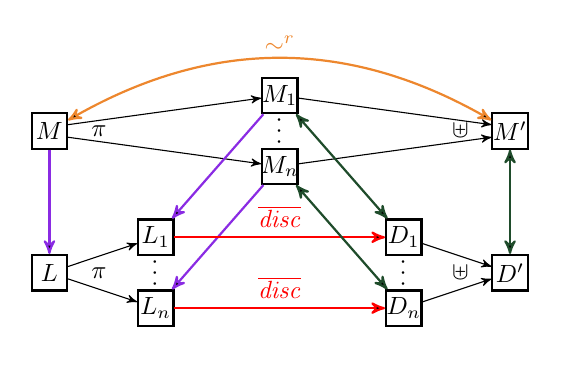
\begin{tikzpicture}[->,>=stealth',auto,x=10mm,y=1cm,node distance=15mm and 3mm,thick,  every node/.style={scale=.9}]
		% Top: Models
		\node[tr, label=center:$M$] (M) {};
		\node[tr, right of = M, label=center:$M_1$, yshift=0.5cm, xshift=1.75cm]  (M1) {}; 
		\node[below of = M1,rotate=90,xshift=10mm] (d1) {$\cdots$};
		\node[tr, right of = M, label=center:$M_n$, yshift=-0.5cm, xshift=1.75cm]  (Mn) {}; 
		\node[tr, right of = M, label=center:$M'$, xshift=5cm]  (M') {};
		
		% Bot: Logs+Discovered Models
		\node[tr, below of = M, label=center:$L$, yshift=-0.5cm]    (L) {}; 
		\node[tr, right of = L, label=center:$L_1$, yshift=0.5cm]   (L1) {}; 
		\node[below of = L1,rotate=90,xshift=10mm] (d2) {$\cdots$};
		\node[tr, right of = L, label=center:$L_n$, yshift=-0.5cm]  (Ln) {};
		
		\node[tr, right of = L1, label=center:$D_1$, xshift=2cm] (D1) {};
		\node[below of = D1,rotate=90,xshift=10mm] (d3) {$\cdots$};
		\node[tr, right of = Ln, label=center:$D_n$, xshift=2cm] (Dn) {};
		\node[tr, below of = M', label=center:$D'$, yshift=-0.5cm]  (D') {};
		
		% "Text"
		\node[right of = M, xshift=-0.8cm] () {$\pi$};
		\node[right of = L, xshift=-0.8cm] () {$\pi$};
		
		\node[left of = M', xshift=0.8cm] () {$\uplus$};
		\node[left of = D',xshift=0.8cm] () {$\uplus$};	
		
		%		% Hacking in the legend
		%		\node[below of = L, label=right:{\textcolor{cadmiumorange}{$\longleftrightarrow$ bisimulation}}, yshift=0.2cm, xshift=-0.6cm]	(a) {};
		%		\node[below of = L, label=right:{\textcolor{blue-violet}{$\longrightarrow$~ generates}}, yshift=-0.2cm, xshift=-0.6cm]	(b) {};
		%		\node[right of = a, label=right:{\textcolor{red}{$\longrightarrow$ discovery}}, yshift=-0.2mm, xshift=1.5cm]	() {};
		%		\node[right of = b, label=right:{\textcolor{green1}{$\longrightarrow$ isomorphism}},xshift=1.5cm]	() {};
		% Empty node to fix caption overlap
		\node[below of = Ln,yshift=1.2cm] (a) {};
		
		%%% If we want to add text next to the arrow, use:
		%%  \path[->, draw=blue-violet] (M) edge node[anchor=center, xshift=-1cm]{\textcolor{blue-violet}{generates}} (L);
		
		% Normal
		\path[->, thin]
		($(M.east)+(0,.8mm)$) edge (M1)
		($(M.east)-(0,.8mm)$) edge (Mn)
		
		(L) edge (L1)
		(L) edge (Ln)
		
		(M1) edge ($(M'.west)+(0,.8mm)$)
		(Mn) edge ($(M'.west)-(0,.8mm)$)
		
		(D1) edge (D')
		(Dn) edge (D')
		;
		% Generates:
		\path[->, draw=blue-violet]
		(M) edge (L)
		(M1) edge (L1)
		(Mn) edge (Ln)
		;
		% Bisimulation
		\path[<->, draw=cadmiumorange]
		(M) edge[bend left=30] node[above,cadmiumorange,yshift=-.5mm]{$\sim^r$} (M')
		;
		% Discovery
		\path[->, draw=red]
		(L1) edge node[above,red]{$\overline{\mathit{disc}}$} (D1)
		(Ln) edge node[above,red]{$\overline{\mathit{disc}}$} (Dn)
		;
		% Isomorphism
		\path[<->, draw=green1]
		(M1) edge (D1)
		(Mn) edge (Dn)
		(M') edge (D')
		;
	\end{tikzpicture}
	
	%	\includegraphics[width=.8\textwidth]{figs/framework}
	\caption{Framework for rediscoverability of typed Jackson Nets. Model $M$ generates an event log $L$. Log projections $L_1 \ldots L_n$ are generated from projected nets $M_1 \ldots M_n$. %(\textcolor{blue-violet}{purple} arrows). 
		Discovery algorithm $\mathit{disc}$ results in nets $D_1 \ldots D_n$, isomorphic to $M_1 \ldots M_n$, 
		%(\textcolor{red}{red} arrows), 
		which can be composed in $D'$.
		$D'$ is isomorphic to $M'$ and thus to $M$.
%		\dbtodo{Rewrite later; should be a ``small story''.}
%		\textcolor{blue-violet}{Purple} arrows indicate that model $M$ generates log $L$.
%		Black arrows denote projections ($\pi$) and compositions ($\composeOperator$).
%		The \textcolor{cadmiumorange}{orange} arrow indicates bisimilarity.
%		Discovery is denoted with \textcolor{red}{red} arrows.
%		Finally, \textcolor{green1}{green} arrows imply isomorphism.
	}
	\figlabel{framework}
\end{figure}


\begin{lemma}
	Let $N$ be a \tjn and $\project{\Upsilon}{N} = (P_\Upsilon, T_\Upsilon, F_\Upsilon, \alpha_\Upsilon, \beta_\Upsilon)$ for some $\Upsilon \subseteq \type_{\Lambda}(N)$ such that $\project{\Upsilon}{N}$ is atomic. 
	Let $\eta \in \mathcal{L}(N, \emptybag)$ be a firing sequence. 
	Then $\mathit{Log}_\Upsilon(\eta)$ is generated by $(N_\Upsilon, \emptybag)$ with $N_\Upsilon = (P_\Upsilon \union \{i, f\},T_\Upsilon,F_\Upsilon \{ (i,t) 
	\mid \pre{t}=\emptyset \} \union \{(t,f) \mid \post{t} = \emptyset\})$.
\end{lemma}
\begin{proof} (sketch)
Let $\sigma \in \mathit{Log}_\Upsilon(\eta)$.
By construction, each firing sequence in $\mathit{Log}_\Upsilon(\eta)$ has some corresponding identifier vector that generated the sequence.
Assume $\vec\upsilon \in \idset^{|\Upsilon|}$ is such a vector for $\sigma$. 

Observe that for any transition $t \in T$ if $\pre{t} = \emptyset$, $\newvar{t} \intersect \Upsilon \neq \emptyset$, and similarly, if $\post{t} = \emptyset$, $\delvar{t} \intersect \Upsilon \neq \emptyset$. As $N$ is identifier sound, only $\pre{\sigma(1)} = \emptyset$ and $\post{\sigma(\length{\sigma})} = \emptyset$.
Define relation $R = \{(M,m) \mid \forall p \in P : M(p)(\upsilon)= m(p) \}$ and  $U = \{ (t,\psi) \mid \upsilon \not\subseteq \rng{\psi} \}$, i.e., $U$ contains all transitions that do not belong to $\sigma$. Then $R$ is a weak simulation, i.e., $\hide{U}{\transitionsystem{N,\emptybag}} \preccurlyeq^r_R \transitionsystem{N_\Upsilon,\emptybag}$ and thus $\pnenabled{(N_\Upsilon,\emptybag)}{\sigma}$.
\end{proof}

Given a set of types $\Upsilon$, if its projection is atomic, the projection can be transformed into a workflow net, and for any firing sequence of the original net, this \wfnet can generate the $\Upsilon$-induced event log.
Suppose we have a discovery algorithm $\mathit{disc}$ that can rediscover models, i.e., given an event log $L$ that was generated by some model $M$, then $\mathit{disc}$ returns the original model. 
Rediscoverability of an algorithm requires some property $P_{\mathit{disc}}(M)$ on the generating model $M$, and some property $Q_{\mathit{disc}}(L, M)$ on the quality of event log $L$ with respect to the generating model $M$. 
In other words, $P(M)$ and $Q(L,M)$ are premises to conclude rediscoverability for discovery algorithm $\mathit{disc}$.
For example, $\alpha$-miner~\cite{AalstWM04} requires for $P(M)$ that model $M$ is well-structured, and for $Q(L,M)$ that event log $L$ is directly-follows complete with respect to model $M$. 
Similarly, Inductive Miner~\cite{Leemans2013} requires the generating model $M$ to be a process tree  without silent actions or self-loops ($P(M)$), and that event log $L$ is directly-follows complete with respect to the original model $M$ ($Q(L,M)$).

\begin{definition}[Rediscovery]\deflabel{rediscovery}
An algorithm $\mathit{disc}$ can \emph{rediscover} \wfnet $W=(P,T,F,in,out)$ from event log $L \subseteq \seq{T}$ if $P_{\mathit{disc}}(W)$ and $Q_{\mathit{disc}}(L,W)$ imply $\mathit{disc}(L) \leftrightsquigarrow W$.
\end{definition}

Thus, suppose there exists a discovery algorithm $\mathit{disc}$ that is -- under conditions $P$ and $Q$ -- able to reconstruct a workflow model given an event log. 
In other words, given an event log $L$ generated by some model $M$, $\mathit{disc}$ returns a model that is isomorphic to the generating model. 
Now, suppose we have a firing sequence $\eta$ of some \tjn $N$, and some projection $\Upsilon$. Then, if $P(\project{\Upsilon}{N})$, and $Q(\mathit{Log}_\Upsilon(\eta),\project{\Upsilon}{N})$, then $\mathit{disc}$ returns a model that is isomorphic to the closure of $\project{\Upsilon}{N}$, as $\mathit{disc}$ only returns \wfnets. 
With $\overline{\mathit{disc}}$ we denote the model where the source and sink places are removed, i.e., $\overline{\mathit{disc}} \leftrightsquigarrow \project{\Upsilon}{N}$.
Then, as shown in \figref{framework}, if we discover for every possible combination of types, i.e., the subset-closed set of all type combinations, 
a model that is isomorphic to the type-projected model, then the composition results in a model that is bisimilar to the original model. 


\begin{theorem}[Rediscoverability of typed Jackson Nets]
Let $N$ be a \tjn, and let $\eta \in \mathcal{L}(N,\emptyset)$ without minor places. 
Let $\mathit{disc}$ be a discovery algorithm with properties $P$ and $Q$ that satisfy \defref{rediscovery}. 
If for all $\emptyset \subset \Upsilon \subseteq \type_{\Lambda}(N)$ 
	the $\Upsilon$-projection is atomic and 
	satisfies conditions $P(\project{\Upsilon}{N})$ and $Q(\mathit{Log}_{\Upsilon}(\eta)), \project{\Upsilon}{N})$,
then $\transitionsystem{N,\emptyset} 
%\sim^r 
\leftrightsquigarrow
\transitionsystem{N',\emptyset}$ with $N' = \biguplus_{\emptyset \subset \Upsilon \subseteq \type_{\Lambda}(N)} \overline{\mathit{disc}}(\mathit{Log}_\Upsilon(\eta))$.

%
%\begin{equation*}
%	\transitionsystem{N,\emptyset} \sim^r \biguplus_{\emptyset \subset \Upsilon \subseteq \type_{\Lambda}(N)} \overline{\mathit{disc}}(\mathit{Log}_\Upsilon(\eta))
%\end{equation*}
\end{theorem}
\begin{proof} (sketch)
Let $\emptyset \subset \Upsilon \subseteq \type_{\Lambda}(N)$ be a set of types in $N$. 
Since $P(\project{\Upsilon}{N})$ and $Q(\mathit{Log}_{\Upsilon}(\eta)), \project{\Upsilon}{N})$%
%, we have $\project{\Upsilon}{N} \leftrightsquigarrow \mathit{disc}(\mathit{Log}_{\Upsilon}(\eta))$. 
the closure of $\project{\Upsilon}{N}$ and $\mathit{disc}(\mathit{Log}_{\Upsilon}(\eta))$ are isomorphic.
From the closure, places $\inp$ and $\outp$ exist with $\pre{\inp} = \emptyset = \post{\outp{}}$. As the nets are isomorphic, we have $\proj{\Upsilon}{N} \leftrightsquigarrow \overline{\mathit{disc}}(\mathit{Log}_{\Upsilon}(\eta))$.
Combining the results gives
$\biguplus_{\emptyset \subset \Upsilon \subseteq \type_{\Lambda}(N)} \overline{\mathit{disc}}(\mathit{Log}_\Upsilon(\eta)) \leftrightsquigarrow
\biguplus_{\emptyset \subset \Upsilon \subseteq \type_{\Lambda}(N)} \project{\Upsilon}{N}$.
The statement then follows directly from \corref{reconstructability}.
%The isomorphism implies that if the right hand side is rooted bisimilar to $(N,\emptyset)$, the left hand side is rooted bisimilar to $(N,\emptyset)$ as well, which proves the statement.
\end{proof}


%
%We propose a framework for rediscoverability based on the reconstructability of \tjns. In a nutshell, we project the event log $L$ onto each type to obtain $n$ sublogs $L_1, \cdots, L_n$, assuming a total of $n$ types in $L$. Similarly, we project model $M$ onto all types to obtain $n$ models $M_1, \cdots, M_n$. We show that if $M$ generates $L$, then by projecting as explained, each $M_i$ also generates $L_i$. For each of these sublogs, we apply some discovery algorithm $D$ obtaining new models $D_1, \cdots, D_n$. We show that each $M_i$ and $D_i$ are equivalent, given that $D$ has \dbtodo{this property}. Furthermore, the composition of all $M_i$ is isomorphic to original net $M$, and isomorphic to the composition of all $D_i$.
%
%%\db{This should eventually be made in TIKZ probably}
%\begin{figure}[h]%[!t]
%    \centering
%    \includegraphics[width=\linewidth]{figs/nu-miner-overview-illustration.pdf}
%    \caption{\dbtodo{Make in Tikz?} Illustration of the framework. Model $M$ generates log $L$ \dbtodo{make caption stand-alone.}}
%    \label{fig:framework_overview}
%\end{figure}
%
%Given a \tjn $N$, we consider an event log to be a firing sequence of $N$. As such, we do not distinguish cases or process instances, as these are indirectly given through the \dbtodo{mode (undefined for now)} of each firing transition. 
%
%\begin{definition}[Event Log]
%	An \emph{event log} $L$ is a tuple $(E, <, act, bind)$, where:
%	\begin{compactitem}
%		\item $(E, <)$ is a total order on events $E$,
%		\item $act: E \rightarrow T$ maps events to transitions, and
%		\item $bind: E \rightarrow ( \V \rightarrow \I \cup \set{\bot})$ is a function associating valuations to events.
%	\end{compactitem}
%\end{definition}
%
%In other words, we consider an event log to be a totally ordered set of events $E$, and each event has an associated action (represented by a transition $t$), as well as valuation that assigns an identifier to variables. We use $\bot$ if the variable is undefined.
%
%Given an event log $L = (E, <, act, bind)$, we define following sets:
%\begin{compactitem}
%	\item $var(e) = \set{v \in \V | bind(e)(v) \neq \bot}$
%	\item $type(e) = \set{\lambda \in \Lambda | \exists v \in var(e) : type_{\V} = \lambda}$
%	\item $types(L) = \Union_{e \in E} type(e)$
%\end{compactitem}
%
%Notice that, since $(E, <)$ is a total order, there is a unique sequence that characterizes the event log $L$. 
%
%$seq(L)$ is the firing sequence induced by $(E, <)$:
%$$
%\forall 1 \le i < j < \size{E} : seq(L)(i) < seq(L)(j)
%$$
%
%We say that an event log $L$ is \emph{generated} by a \tpnid if it is a firing sequence of that net.
%
%\begin{definition}[Generated Log] \deflabel{generated_by}
%	Let $N=(P, T, F,\alpha, \beta)$ a \tpnid, and $L = (E, <, act, bind)$. Given two markings $m, m'\in \markings{N}$, we define
%	$$
%	\fires{N}{m}{e}{m'} \iff \fires{N}{m}{(act(e), bind(e))}{m'}
%	$$
%	We say $L$ \emph{is generated by} $\markednet{N}{m_0}$ if markings $m_1, \cdots, m_{\size{E}}$ exist such that:
%	$$
%	\left(
%		N : m_1
%		\overset{{seq(l)(1)}}{\longrightarrow}
%		m_2
%		\overset{{seq(l)(2)}}{\longrightarrow}
%		\cdots
%		\overset{{seq(l)(\size{E})}}{\longrightarrow}
%		m_{\size{E}}
%	\right)
%	$$
%\end{definition}
%
%
%To construct an event log for a given set of identifiers, we use type projection on logs.
%
%\begin{definition} [Log Projection]
%	\dbtodo{def here}
%\end{definition}
%
%Notice that \defref{generated_by} implies that the event log can be replayed by a marked \tpnid. For \tjns it holds that, given a set of types, the projected logs can be replayed by the projected nets.
%
%\begin{lemma}
%	Let $N = (P, T, F, \alpha, \beta)$ a \tjn, and let $L$ an event log generated by $\markednet{N}{\emptyset}$. Then $\project{\L}{L}$ is generated by $\markednet{\project{\L}{N}}{\emptyset}$, for any $\L \subseteq types(n)$.
%\end{lemma}
%\begin{proof}
%	\dbtodo{the proof here}
%\end{proof}
%
%\begin{property}[\dbtodo{rediscoverability?}]
%	Let $M$ be a \tjn that generated log $L$. Suppose some discovery algorithm uses $L$ to discover new model $D$, then $M$ and $D$ are isomorphic. We write this as $Q(L, M)$, where relation $Q$ defines the isomorphism.
%\end{property}
%
%\begin{corollary}
%	M' is isomorphic to D' after removing minor places.
%\end{corollary}
%
%
%WE BUILD A DISCOVERY FRAMEWORK BASED ON THE DECOMPOSABILITY OF TYPED JACKSON NETS: PROJECT THE EVENT LOG SUCH THAT FOR EACH TYPE WE OBTAIN ITS LIFE CYCLE. NEXT, PROJECT ALSO ON ALL OF THE POSSIBLE ``INTERACTION LIFE CYCLES'', AND USE THE COMPOSITION OPERATOR OF TYPED JACKSON NETS TO OBTAIN A NET THAT DESCRIBES THE OBSERVED BEHAVIOR.
%
%THAT'S THE IDEA. WHEN AND HOW DOES IT WORK?
%
%WHAT ARE THE REQUIRED ASSUMPTIONS ON THE EVENT LOG?
%
%- EVENT LOG GENERATED BY A PROCESS THAT CAN BE REPRESENTED BY A TYPED JACKSON NET.
%
%- IDENTIFIER COMPLETENESS, I.E., THE DIRECTLY-FOLLOWS RELATION IS COMPLETE FOR EACH TYPE.
%
%- INTERACTION COMPLETENESS, I.E., THE DIRECTLY-FOLLOWS RELATION FOR EACH SET OF TYPES IS COMPLETE
%
%THEN, THE IDEA IS THAT IF A DISCOVERY ALGORITHM GUARANTEES SOME PROPERTY $\B$ ON EACH OF THE PROJECTED SUB LOGS, THEN THE COMPOSITION OPERATOR RETURNS A MODEL THAT IS BISIMILAR TO THE NET THAT ``GENERATED THE EVENT LOG''
%
%WHAT ARE THE REQUIREMENTS FOR \B?
%%
%
%Here we present a parametric approach for compositional discovery of t-JNs. \todo{shall we call it compositional?}
%In the nutshell, given a log $L$ over a set of event signatures $\E$ and a discovery algorithm $\D$,
%the approach first discovers a set of process models, each of which is obtained for a log projection $\restr{L}{O}$, for each $(n,O)\in\E$.
%Then, all the log projections are brought together using the composition operator $\bigoplus$.
%Conceptually, the approach is similar to the one discussed for the discovery of object-centric nets in~\cite{berti}. At the same time, it does not only work for a different class of process models in which identifiers (as well as relations between them) are explicit, but also comes with formal guarantees regarding the rediscoverability.\andy{rewrite the above paragraph}
%
%
%\begin{algorithm}
%    \caption{TJN-miner $\D_{id}$}\label{alg:cap}
%    \begin{algorithmic}
%        \Require a log $L$ over a set of event signatures $\E$, discovery algorithm $\D$
%        \Ensure a t-JN $N'$
%        \State $\N \gets \emptyset$
%        \For{$O\in \set{O\mid (n,O)\in\E}$}
%        \State $\N \gets \N\cup\D(\restr{L}{O})$
%        \EndFor
%        \State $N'=\bigoplus_{N\in\N} N$
%    \end{algorithmic}
%\end{algorithm}
%Here, $\D$ is the discovery algorithm for low-level Petri nets. %\todo{what are the properties of $\D$?}
%It is easy to see that while taking a projection over some $O$, then values provided by $\zeta$ in each event $(n,\zeta)$ (with $\dom{\zeta}=O$)  essentially create a case identifier.
%%\andy{Is the synchronization operator $\oplus$ always the same?}
%
%Notice that, if the input log $L$ is over a set of event signatures $\E$ such that $|\E|=1$, then the discovered t-JN should contain one single type.
%This also means that, in that case, it suffices to use any traditional discovery algorithm for P/T-nets.  %and the net discovered with $\D_{id}$ is topologically equivalent to the one discovered with $\D$ (i.e., their net graphs coincide)\todo{isomorphism?}
%
%\begin{proposition}
%    Let $L$ be a log. Then if $|\E|=1$, then $\D_{id}(L)=\D(L)$.
%    \andy{is that formulation even correct?}
%\end{proposition}
%
%
%% %\andy{if we consider dominant places (that is, places that have non-singleton types and that dominate over other single-typed places for cases when identical behaviors are discovered for both single types and those derived from valid relations), do we get isomorphism as well?}
%
%In the next sections we show how this framework can be instantiated with concrete discovery algorithms for $\D$ and demonstrate related rediscoverability results. For all the further instantiations we will be interested in t-JN logs, that is, logs logs composed of traces produced by t-JNs. The next definition sets up formally the main properties of t-JN logs.
%
%\begin{definition}[T-JN log]
%    A t-JN log over a set of signatures $\E$ is such a $\E$-complete log $L$ for which the following holds:
%    \begin{itemize}
%        \item every case starts with firing one of the emitters and ends by firing the last collector;
%        \item for every $t\in T$, there is a trace in $L$ that contains $t$ as an activity name;
%        \item every $O$-typed projection of the log is complete with respect to the non-typed directly follows relation.
%    \end{itemize}
%    \andy{make a proper definition that starts with a log formed by all traces produced by a t-JN (PNID traces should be defined Section 3 )}
%\end{definition}
%
%
%After having defined a particular type of logs we will be interested in, we would like to define a generic property of $\D_{id}$ discovery algorithm. This property will prove itself useful when studying theoretical properties of concrete instantiations of $\D_{id}$.
%
%\begin{definition}[Typed discovery property]\label{def:discovery-property}
%    this property should be defined similarly to the one of Inductive Miner
%\end{definition}
%
%
%Further on, for every instantiation of our parametric algorithm, we will be interested in the classical property of discovery algorithm known as \emph{rediscoverability}.
%In the nutshell, given a marked identifier sound typed Jackson net $(N,M_0)$ and a discovery algorithm $\D_{id}$ that discovers from a log induced by $N$ a typed Jackson net that is identifier sound, we say that $\D_{id}$ \emph{rediscovers} $N$ if for every log induced by $N$, $\D_{id}$ returns $N'$ that is equivalent to $N$ (modulo renaming of places).
%
%% \andy{Do we have any generic basic property of the algorithm? For example, we could say that $\D$ must be such that $\D(\restr{L_N}{O})\sim\restr{N}{O}$, for every $O\in\set{O\mid (n,O)\in\E}$. This, on the one hand, doesn't affect the algorithm. On the other hand, we might limit the ``admissible'' algorithms for out framework.}
%
%
%





% \endinput

% \subsection{Rediscoverability}
% %\andy{Can we say something about the compositionality here? Why can we rediscover the original net while taking its ``propositionalized'' projections? Is it a property that comes from Jackson nets? Or from the composition operator? Or is it just a coincidence? }
% Let us first recall the classical property of discovery algorithm known as \emph{rediscoverability}.
% Given a marked identifier sound typed Jackson net $(N,M_0)$, we say that a discovery algorithm $\mathtt{DA}$ that discovers from a log induced by $N$ typed Jackson nets that are identifier sound. Then, if for every log  induced by $N$, $\mathtt{DA}$ returns $N'$ that is equivalent to $N$ (modulo renaming of places), then $\mathtt{DA}$ \emph{rediscovers} $N$.





% %\andy{if we do a projection on log for a single variable, then we obtain ``plain'' logs on which $\alpha$-miner can be executed (a la Berti)}




% \subsection{Curious example}

% Consider the following net $N$:


% \begin{center}
%     \begin{tikzpicture}[->,>=stealth',auto,x=15mm,y=1.0cm,node distance=15mm and 7mm,thick, scale=0.8, every node/.style={scale=0.8}]

%         \node[tr] (a) {$a$};
%         \node[pl,right of = a,xshift =8mm] (p1) {};
%         \node[tr,right of = p1,xshift =8mm] (d) {$d$};

%         \node[pl,below of = a,xshift =8mm] (p2) {};
%         \node[tr,right of = p2] (c) {$c$};
%         \node[pl,right of = c]  (p3) {};

%         \node[tr,below of = p2,xshift=-8mm] (b) {$b$};
%         \node[pl,right of = b,xshift =8mm] (p4) {};
%         \node[tr,right of = p4,xshift =8mm] (e) {$e$};


%         \path[->]
%         (a) edge (p1)
%         (p1) edge (d)
%         (a) edge (p2)
%         (p2) edge (c)
%         (c) edge (p3)
%         (b) edge (p2)
%         (p3) edge (d)
%         (p3) edge (e)
%         (b) edge (p4)
%         (p4) edge (e)
%         ;
%     \end{tikzpicture}
% \end{center}

% Consider $L_N$. Then the rediscovered net with $\alpha$-miner looks as follows:
% \begin{center}
%     \begin{tikzpicture}[->,>=stealth',auto,x=15mm,y=1.0cm,node distance=15mm and 7mm,thick, scale=0.8, every node/.style={scale=0.8}]

%         \node[tr] (a) {$a$};
%         \node[pl,right of = a,xshift =8mm,draw=none] (p1) {};
%         \node[tr,right of = p1,xshift =8mm] (d) {$d$};

%         \node[pl,below of = a,xshift =8mm] (p2) {};
%         \node[pl,left of = p2,xshift=-3mm] (p5) {};
%         \node[tr,right of = p2] (c) {$c$};
%         \node[pl,right of = c]  (p3) {};

%         \node[tr,below of = p2,xshift=-8mm] (b) {$b$};
%         \node[pl,right of = b,xshift =8mm,draw=none] (p4) {};
%         \node[pl,right of = p3,xshift=3mm] (p6) {};
%         \node[tr,right of = p4,xshift =8mm] (e) {$e$};


%         \path[->]

%         (a) edge (p2)
%         (p2) edge (c)
%         (c) edge (p3)
%         (b) edge (p2)
%         (p3) edge (d)
%         (p3) edge (e)

%         (d) edge (p6)
%         (e) edge (p6)
%         (p5) edge (a)
%         (p5) edge (b)
%         ;
%     \end{tikzpicture}
% \end{center}

% This demonstrates one of the limitation of $\alpha$-miner: it cannot discover non-local dependencies. Indeed, for the given example the miner does not discover the place between $a$ and $d$, and the place between $b$ and $e$.

% Now, let us consider $N'$ -- a typed version of $N$:

% \begin{center}
%     \begin{tikzpicture}[->,>=stealth',auto,x=15mm,y=1.0cm,node distance=15mm and 7mm,thick, scale=0.8, every node/.style={scale=0.8}]

%         \node[tr] (a) {$a$};
%         \node[pl,right of = a,xshift =8mm] (p1) {};
%         \node[tr,right of = p1,xshift =8mm] (d) {$d$};

%         \node[pl,below of = a,xshift =8mm] (p2) {};
%         \node[tr,right of = p2] (c) {$c$};
%         \node[pl,right of = c]  (p3) {};

%         \node[tr,below of = p2,xshift=-8mm] (b) {$b$};
%         \node[pl,right of = b,xshift =8mm] (p4) {};
%         \node[tr,right of = p4,xshift =8mm] (e) {$e$};


%         \path[->]
%         (a) edge node{$x$} (p1)
%         (p1) edge node{$x$} (d)
%         (a) edge node{$y$}                                                                                                                                                                                                                                                                                                                                                                                                                                                                                                                                                                                                                                                                                                                                                                                                                                                                                                                                                                                                                                                                                                                                                                                                                                                                                                                                     (p2)
%         (p2) edge node{$y$}                                                                                                                                                                                                                                                                                                                                                                                                                                                                                                                                                                                                                                                                                                                                                                                                                                                                                                                                                                                                                                                                                                                                                                                                                                                                                                                                     (c)
%         (c) edge node{$y$}                                                                                                                                                                                                                                                                                                                                                                                                                                                                                                                                                                                                                                                                                                                                                                                                                                                                                                                                                                                                                                                                                                                                                                                                                                                                                                                                     (p3)
%         (b) edge node{$y$}                                                                                                                                                                                                                                                                                                                                                                                                                                                                                                                                                                                                                                                                                                                                                                                                                                                                                                                                                                                                                                                                                                                                                                                                                                                                                                                                     (p2)
%         (p3) edge node{$y$}                                                                                                                                                                                                                                                                                                                                                                                                                                                                                                                                                                                                                                                                                                                                                                                                                                                                                                                                                                                                                                                                                                                                                                                                                                                                                                                                     (d)
%         (p3) edge node{$y$}                                                                                                                                                                                                                                                                                                                                                                                                                                                                                                                                                                                                                                                                                                                                                                                                                                                                                                                                                                                                                                                                                                                                                                                                                                                                                                                                     (e)
%         (b) edge node{$x$} (p4)
%         (p4) edge node{$x$} (e)
%         ;
%     \end{tikzpicture}
% \end{center}
% Let us now apply $\D_{id}$ to $N'$.
% We start by discovering nets for log projections.
% For the type of $x$, we get $\D(\restr{L_{N'}}{x})$:
% \begin{center}
%     \begin{tikzpicture}[->,>=stealth',auto,x=15mm,y=1.0cm,node distance=15mm and 7mm,thick, scale=0.8, every node/.style={scale=0.8}]

%         \node[tr] (a) {$a$};
%         \node[pl,right of = a,xshift =8mm] (p1) {};
%         \node[tr,right of = p1,xshift =8mm] (d) {$d$};


%         \node[tr,below of = a] (b) {$b$};
%         \node[pl,right of = b,xshift =8mm] (p4) {};
%         \node[tr,right of = p4,xshift =8mm] (e) {$e$};

%         \node[pl,left of = a,yshift=-8mm] (p5) {};
%         \node[pl,right of = d,yshift=-8mm] (p6) {};


%         \path[->]
%         (a) edge node{$x$} (p1)
%         (p1) edge node{$x$} (d)
%         (b) edge node{$x$} (p4)
%         (p4) edge node{$x$} (e)
%         (p5) edge node{$x$} (a)
%         (p5) edge node{$x$}  (b)
%         (d) edge node{$x$}  (p6)
%         (e) edge node{$x$}  (p6)
%         ;
%     \end{tikzpicture}
% \end{center}

% For $y$ we obtain the following net  $\D(\restr{L_{N'}}{y})$:
% \begin{center}
%     \begin{tikzpicture}[->,>=stealth',auto,x=15mm,y=1.0cm,node distance=15mm and 7mm,thick, scale=0.8, every node/.style={scale=0.8}]

%         \node[tr] (a) {$a$};
%         \node[pl,right of = a,xshift =8mm,draw=none] (p1) {};
%         \node[tr,right of = p1,xshift =8mm] (d) {$d$};

%         \node[pl,below of = a,xshift =8mm] (p2) {};
%         \node[pl,left of = p2,xshift=-3mm] (p5) {};
%         \node[tr,right of = p2] (c) {$c$};
%         \node[pl,right of = c]  (p3) {};

%         \node[tr,below of = p2,xshift=-8mm] (b) {$b$};
%         \node[pl,right of = b,xshift =8mm,draw=none] (p4) {};
%         \node[pl,right of = p3,xshift=3mm] (p6) {};
%         \node[tr,right of = p4,xshift =8mm] (e) {$e$};


%         \path[->]

%         (a) edge node{$y$}                                                                                                                                                                                                                                                                                                                                                                                                                                                                                                                                                                                                                                                                                                                                                                                                                                                                                                                                                                                                                                                                                                                                                                                                                                                                                                                                     (p2)
%         (p2) edge node{$y$}                                                                                                                                                                                                                                                                                                                                                                                                                                                                                                                                                                                                                                                                                                                                                                                                                                                                                                                                                                                                                                                                                                                                                                                                                                                                                                                                     (c)
%         (c) edge node{$y$}                                                                                                                                                                                                                                                                                                                                                                                                                                                                                                                                                                                                                                                                                                                                                                                                                                                                                                                                                                                                                                                                                                                                                                                                                                                                                                                                     (p3)
%         (b) edge node{$y$}                                                                                                                                                                                                                                                                                                                                                                                                                                                                                                                                                                                                                                                                                                                                                                                                                                                                                                                                                                                                                                                                                                                                                                                                                                                                                                                                     (p2)
%         (p3) edge node{$y$}                                                                                                                                                                                                                                                                                                                                                                                                                                                                                                                                                                                                                                                                                                                                                                                                                                                                                                                                                                                                                                                                                                                                                                                                                                                                                                                                     (d)
%         (p3) edge node{$y$}                                                                                                                                                                                                                                                                                                                                                                                                                                                                                                                                                                                                                                                                                                                                                                                                                                                                                                                                                                                                                                                                                                                                                                                                                                                                                                                                     (e)

%         (d) edge node{$y$}                                                                                                                                                                                                                                                                                                                                                                                                                                                                                                                                                                                                                                                                                                                                                                                                                                                                                                                                                                                                                                                                                                                                                                                                                                                                                                                                     (p6)
%         (e) edge node{$y$}                                                                                                                                                                                                                                                                                                                                                                                                                                                                                                                                                                                                                                                                                                                                                                                                                                                                                                                                                                                                                                                                                                                                                                                                                                                                                                                                     (p6)
%         (p5) edge node{$y$}                                                                                                                                                                                                                                                                                                                                                                                                                                                                                                                                                                                                                                                                                                                                                                                                                                                                                                                                                                                                                                                                                                                                                                                                                                                                                                                                     (a)
%         (p5) edge node{$y$}                                                                                                                                                                                                                                                                                                                                                                                                                                                                                                                                                                                                                                                                                                                                                                                                                                                                                                                                                                                                                                                                                                                                                                                                                                                                                                                                     (b)
%         ;
%     \end{tikzpicture}
% \end{center}


% By merging $\D(\restr{L_{N'}}{x})$ and $\D(\restr{L_{N'}}{y})$, we obtain the original $N'$. Notice  that  the discovery algorithm here identifies non-local dependencies between actions.
% \endinput

% \subsection{Discovering directly-follows relations between objects}

% %
% %\begin{definition}
% %Let $L$ be a log. Then $G(L)=(V,E)$ is the \emph{identifier graph} it induces, where $V=\id{L}$ and $E=\set{(\cname{id_1},\cname{id_2})\mid \exists\trace\in L \land \exists (n,\zeta)\in \trace:  \cname{id_1}\in\rng{\zeta} \land \cname{id_2}\in\rng{\zeta}}$.
% %\end{definition}
% %It is easy to see that $G(L)$ is constructed by taking all the object identifiers appearing in the log and creating links only between those that appear in the same event payload.
% %
% %\begin{example}
% %Consider the complete log $L$ from Example~\ref{ex:log}.
% %Then we can construct $G(L)$ that looks as follows:
% %
% %\begin{center}
% %\begin{tikzpicture}[every node/.style={thick}]
% %	\node (1) {$\cname{1}$};
% %	\node[below of = 1] (2) {$\cname{2}$};
% %	\node[right of = 1] (A) {$\cname{A}$};
% %	\node[right of = 2] (B) {$\cname{B}$};
% %	\node[right of = B,yshift = 5mm] (st) {$\bigstar$};
% %	\path[-] 
% %			(1) edge (A) edge (B)  edge (st)
% %			(A) edge (st)
% %			(2) edge (A) edge (B) edge (st)
% %			(B) edge (st);
% %\end{tikzpicture}
% %\end{center}
% %\end{example}
% %
% %With that graph $(V,E)$ at hand, we can proceed by defining relations between object types together with their related multiplicities. 
% %To this end, given two names $o_1,o_2\in\O_\E$ as well as values $\cname{id_1},\cname{id_1'}\in V\cap I(type_{\V}(o_1))$ and $\cname{id_2},\cname{id_2'}\in V\cap I(type_{\V}(o_2))$, we define the following relations:
% %\begin{itemize}
% %\item $(o_1,o_2)\in R_{\mathtt{m,1}}$ iff if $(\cname{id_1},\cname{id_2}),(\cname{id_1},\cname{id_2'})\in E$, then $\cname{id_2}=\cname{id_2'}$;
% %\item $(o_1, o_2)\in R_{\mathtt{1,1}}$ iff if $(\cname{id_1},\cname{id_2}),(\cname{id_1'},\cname{id_2'})\in E$, then  $\cname{id_1}=\cname{id_1'}$ and $\cname{id_2}=\cname{id_2'}$;
% %\item $(o_1, o_2)\in R_{\mathtt{m,m}}$ otherwise.
% %\end{itemize}


% Now we can proceed with generating directly follows relations for each signature in $\E$. The main idea here is to
% We start by projecting the log on one object name at a time (notice that like that the identifier value is identical to a case identifier). Then the procedure for extracting directly follows relation is identical to the one used in $\alpha$-miner.

% \begin{definition}[Typed ordering relations]
%     Let $L$ be a log over a set of event signatures $\E$, $o\in \O_\E$ be an object name and $a_1,a_2\in \N_\E$ two activity names.
%     \begin{enumerate}
%         \item $>_L^o\subseteq \N_\E\times \N_\E$ is an $o$-typed directly follows relation s.t.
%               $a_1 >_L^o a_2$ iff there is a trace $\tup{e_1\cdots e_m}\in \restr{L}{\set{o}}$ s.t. $e_i=(a_1,o)$ and $e_{i+1}=(a_2,o)$, for some $1\leq i \leq m-1$.
%         \item $\to_L^o\subseteq \N_\E\times \N_\E$ is an $o$-typed  causality relation s.t. $a_1 \to_L^o a_2$ iff $a_1 >_L^o a_2$ and $a_2 \not>_L^o a_1$.
%         \item $\#_L^o\subseteq \N_\E\times \N_\E$ is an $o$-typed  conflict relation s.t. $a_1 \#L^o a_2$ iff $a_1 \not>_L^o a_2$ and $a_2 \not>_L^o a_1$.
%         \item $||_L^o\subseteq \N_\E\times \N_\E$ is an $o$-typed  concurrency relation s.t. $a_1 ||_L^o a_2$ iff $a_1 >_L^o a_2$ and $a_2 >_L^o a_1$.
%     \end{enumerate}
% \end{definition}


% Since the above relations can be derived from $>_L^o$ , we assume the log to be complete with respect to $>_L^o$.








% %
% %
% %
% %An algorithm/heuristic is said to rediscover a workflow net if this algorithm is
% %able to regenerate the exact net structure of the original net, abstracting from
% %the place labels (see Definition 2.4). The α-algorithm is proved to (re)discover all
% %SWF-nets if the SWF-net does not contain short-loops. That means that short
% %loops are a first limitation of the α-algorithm. However, if the notion of ability to
% %rediscover is relaxed to behaviorally equivalent (i.e. both generate the same log
% %traces), then the α-algorithm is able to mine other sound WF-nets, like the one
% %in Figure 3. This net is not an SWF-net because transition G can be enabled
% %without the firing of transitions E and F. However, even with this relaxed notion
% %of ability to rediscover and the restriction on short-loops, the α-algorithm cannot
% %be proved to correctly mine all sound WF-nets.
	%\section{The $\nu$-miner} \seclabel{nu_miner}
Here we show that the Inductive Miner has nice property $\B$, which means that we can use it in the framework.




\subsection{TJN-miner under the $\mathtt{ind}$-regime}
Here we study the instantiation of the framework when $\D$ is Inductive Miner.
We call this instantiation the $\mathtt{ind}$-regime and refer to the respective TJN-miner as $\D^{\mathtt{ind}}_{id}$.


\andy{introduce process trees and Jackson types}

The following proposition\todo{or lemma?}  establishes a connection between process trees and untyped Jackson nets.

\begin{proposition}
	Process trees are untyped Jackson nets.
	\andy{reformulate}
\end{proposition}

\andy{do we need a proposition/lemma for the typed case?}

Now, we would like to recall the main properties of the inductive miner discovery algorithm.
\andy{add those properties}
We next show that the $\D_{id}$ property from Definition~\ref{def:discovery-property} holds for the original inductive miner algorithm.

\begin{proposition}
	The property from Definition~\ref{def:discovery-property} holds for Inductive Miner.
	\andy{reformulate}
\end{proposition}

Next we show a couple of rediscoverability-related results.


\begin{proposition}
	Let $N$ be a t-JN and $L$ is its $\E$-complete t-JN log.
	Then $\restr{N}{O} \sim \D_{id}^{\mathtt{ind}}(\restr{L}{O})$, for all $(n,O)\in\E$.
\end{proposition}


\begin{proposition}
	Let $N$ be a t-JN and $L$ is its $\E$-complete t-JN log.
	Then $N\sim \bigoplus_{O\in\O_\E}\D_{id}^{\mathtt{ind}}(\restr{L}{O})$.
\end{proposition}

	%%%%%%%%%%%%%%%%%%%%%%%%%%%%%%%%%%%%%%%%%%%%%%%%%%%%%%%%%%%%%%%%%%%%%%%%%%%%%%%
\section{Conclusion} 
\seclabel{discussion_conclusion}
%%%%%%%%%%%%%%%%%%%%%%%%%%%%%%%%%%%%%%%%%%%%%%%%%%%%%%%%%%%%%%%%%%%%%%%%%%%%%%%
% 2023-03-17: Artem
In this paper, we studied typed Jackson Nets to model systems of interacting processes, a class of well-structured process models describing manipulations of object identifiers.
As we show, this class of nets has an important property of reconstructability.
In other words, the composition of the projections on all possible type combinations returns the model of the original system.
Ignoring the interactions between processes results in less accurate, or even wrong, models.
Similar problems occur in the discovery of systems of interacting processes, such as  object-centric process discovery, where event logs are flattened for each object.

% 2023-03-17: Artem
This paper provides a formal foundation for the composition of block-structured nets, and uses this to develop a framework for the discovery of systems of interacting processes.
We link the notion of event logs used for process discovery to system executions, and show that it is not possible to observe whether an event log is generated by a system of interacting processes, or by a projection of the system.
These properties form the key ingredients of the framework.
We show under what conditions a process discovery algorithm (that guarantees rediscoverability) can be used to discover the individual processes and their interactions, and how these can be combined to rediscover a model of interacting processes that is bisimilar to the original system that generated the event logs.

%Similar to Agent Miner~\cite{TourPKS2022agentdiscovery}, our framework applies a divide-and-conquer strategy.
%It proceeds by projecting the input event log into several event logs, one for each %combination of objects (the divide step), then discovering models from the projected event logs (the conquer step), and, finally, composing the discovered models into the overall system.
%Differently from Agent Miner, the division step is driven by objects manipulated by and not agents participating in the processes.
%Given the discovery algorithms used to conquer the projected event logs guarantee rediscoverability, the overall algorithm rediscovers the original system.
%This result is grounded in the reconstructability property of typed Jackson Nets.
%The discovered systems are live and identifier sound by construction, which are two desired correctness properties for business processes.
% 2023-03-17: Artem
Although typed Jackson Nets have less expressive power than formalisms like Object-centric Petri nets~\cite{aalstB20_discovering}, proclets~\cite{Fahland2019} or interacting artifacts~\cite{LuNWF15}, this paper shows the limitations and potential pitfalls of discovering interacting processes. 
This work aims to lay formal foundations for object-centric process discovery.
As a next step, we plan to implement the framework and tune our algorithms to discover useful models from industrial datasets.

\smallskip
\noindent
\textbf{Acknowledgements.}
Artem Polyvyanyy was in part supported by the Australian Research Council project DP220101516.

%%%%%%%%%%%%%%%%%%%%%%%%%%%%%%%%%%%%%%%%%%%%%%%%%%%%%%%%%%%%%%%%%%%%%%%%%%%%%%%




% MOVE TO DISCUSSION?
%To address this limitation, researchers have developed object-centric approaches, which incorporate information about data objects into the process model. Broadly speaking, there are two main streams of research when it comes to object-centric approaches using \pns. The first idea is to represent objects implicitly, most prominently done by proclets~\cite{proclet_paper_probably_by_dirk_in_stead_of_wil?}, where life-cycles of objects are modeled with (classical) \pns. The generation and synchronization of objects in the process is done using special ``ports'', annotated with multiplicity constraints. Correctness of proclets is still an open topic; \dbtodo{potentially due to the ports that arent defined as normal petri nets}. Objects can also be represented explicitly, as done in~\cite{deFrutosEscrig2005}, where systems comprising of various processes are modeled as a tuple of \pns, with added synchronization transitions. While objects are modeled explicitly, their life-cycle becomes implicit. The $\nu$-net~\cite{RosaVelardo2006,RosaVelardo2007} builds upon \cite{deFrutosEscrig2005} by adding name generation (generation of fresh tokens, with tokens representing objects) in a formal manner. Various models extend these $\nu$-nets, such as typed Petri nets with identifiers (\tpnids)~\cite{vanderWerf2022} and Catalog-nets~\cite{catalog_nets_citation}. \dbtodo{final sentence on correcntess and decidability}.

% MOVE TO DISCUSSION?
%None of these models are sound with respect to the objects they model. As such, in this paper, we focus on \emph{typed Jackson nets} (\tjns), a type of process model that builds upon the classical language of Petri nets but adds data-awareness. A \tjn is a \tpnid that is \emph{identifier sound} by construction~\cite{vanderWerf2022}, meaning that they are able to track the movement of data objects through the process and ensure that the data remains consistent and accurate.
%We propose a framework for discovering these \tjns. The framework uses the notion of \emph{decomposability} -- the composition of the projections of \tjns onto its identifiers give rise to a bisimilar model -- and focuses on \textit{rediscoverability}.
	
	%% Remove this in the actual paper - it's to explain what macro's do
	%% and partly made to fix all issues in them.
	% \input{macro_testing.tex}
	
	%% References
	%% Note: don't include extensions; it confuses tex-studio immensely.
	\bibliographystyle{setup/splncs04}
	\bibliography{references}
\end{document}